%\renewcommand{\chaptername}{Appendix}
%\renewcommand{\thechapter}{5}
%\addcontentsline{toc}{chapter}{Appendix}
\renewcommand{\chaptername}{}

\setcounter{table}{0}
\renewcommand{\thetable}{A\arabic{table}}

\setcounter{figure}{0}
\renewcommand{\thefigure}{A\arabic{figure}}

\chapter{Appendix A} 
\label{sec:appendix}

\section{Extraction protocol}
\label{appendix:extractionProtocol}
\begin{enumerate}
    \item 180 $\mu$L buffer ATL and 15 $\mu$L proteinase K was added to tissue (after all the ethanol had evaporated off), and incubated in a heatblock at 56\textsuperscript{o}C overnight.
    \item Digested tissue was centrifuged for 5 min at 16000 RCF (relative centrifugal force).
    \item The supernatant was pipetted into a clean tube, and 65 $\mu$L NaCl (5M) added. The sample was vortexed for 30s, and then centrifuged for 5 min.
    \item The supernatant was pipetted into another clean tube (leaving behind the white salt residue), and 150 $\mu$L isopropanol (98\%) added. The sample was gently mixed, and left in a freezer for at least 2 hr.
    \item The sample was centrifuged for 5 min, and the liquid removed (leaving behind the DNA pellet).
    \item 250 $\mu$L cooled ethanol (80\%) was added, followed by 30s of vortexing and 5 min centrifuging. The ethanol was then removed, and step 6 was repeated.
    \item After removing the ethanol, the sample was left in a heatblock at 40\textsuperscript{o}C for 15 min in order to dry the DNA pellet.
    \item The sample was suspended in 100 $\mu$L buffer AE, and stored at -18\textsuperscript{o}C.
\end{enumerate}

\section{DNA sequences}

\subsection{Submission to Genbank}
\label{appendix:genbank_submission}
Sequences were uploaded to Genbank via the submission portal available at \url{https://submit.ncbi.nlm.nih.gov/}. The COI protein-coding sequences were uploaded via BankIt (accessed from the same Genbank submission portal). This required information regarding the start codon position, which was found by obtaining the longest open reading frame using ORFfinder (\url{https://www.ncbi.nlm.nih.gov/orffinder/}). The genetic code was set to `Invertebrate Mitochondrial' and ORF codon start codon to `ATG and alternative initiation codons'.

\subsection{Gel images}

\begin{figure}[H]
\centering 
	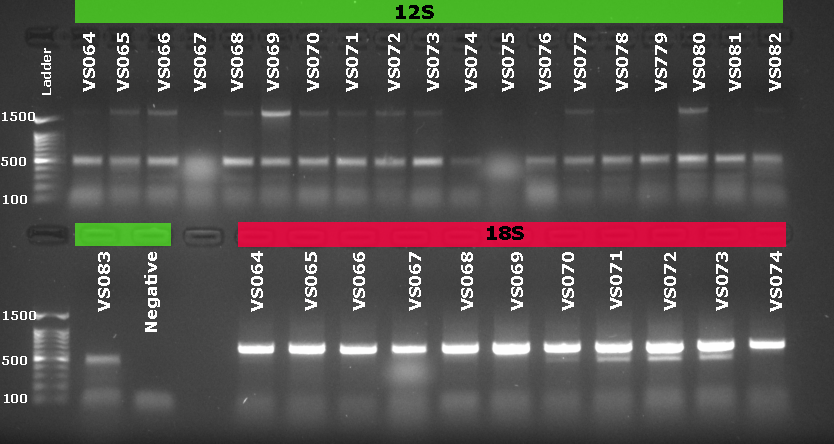
\includegraphics[scale = 1]{Images/12S_gel.pdf}
	\caption{12S and 18S PCR products visualised on 1\% agarose gel. Note the double bands in many of the 12S products; at the 500 and 1500 base pair mark.}
	\label{fig:12Sgel}
\end{figure}

\begin{figure}[H]
	\centering
	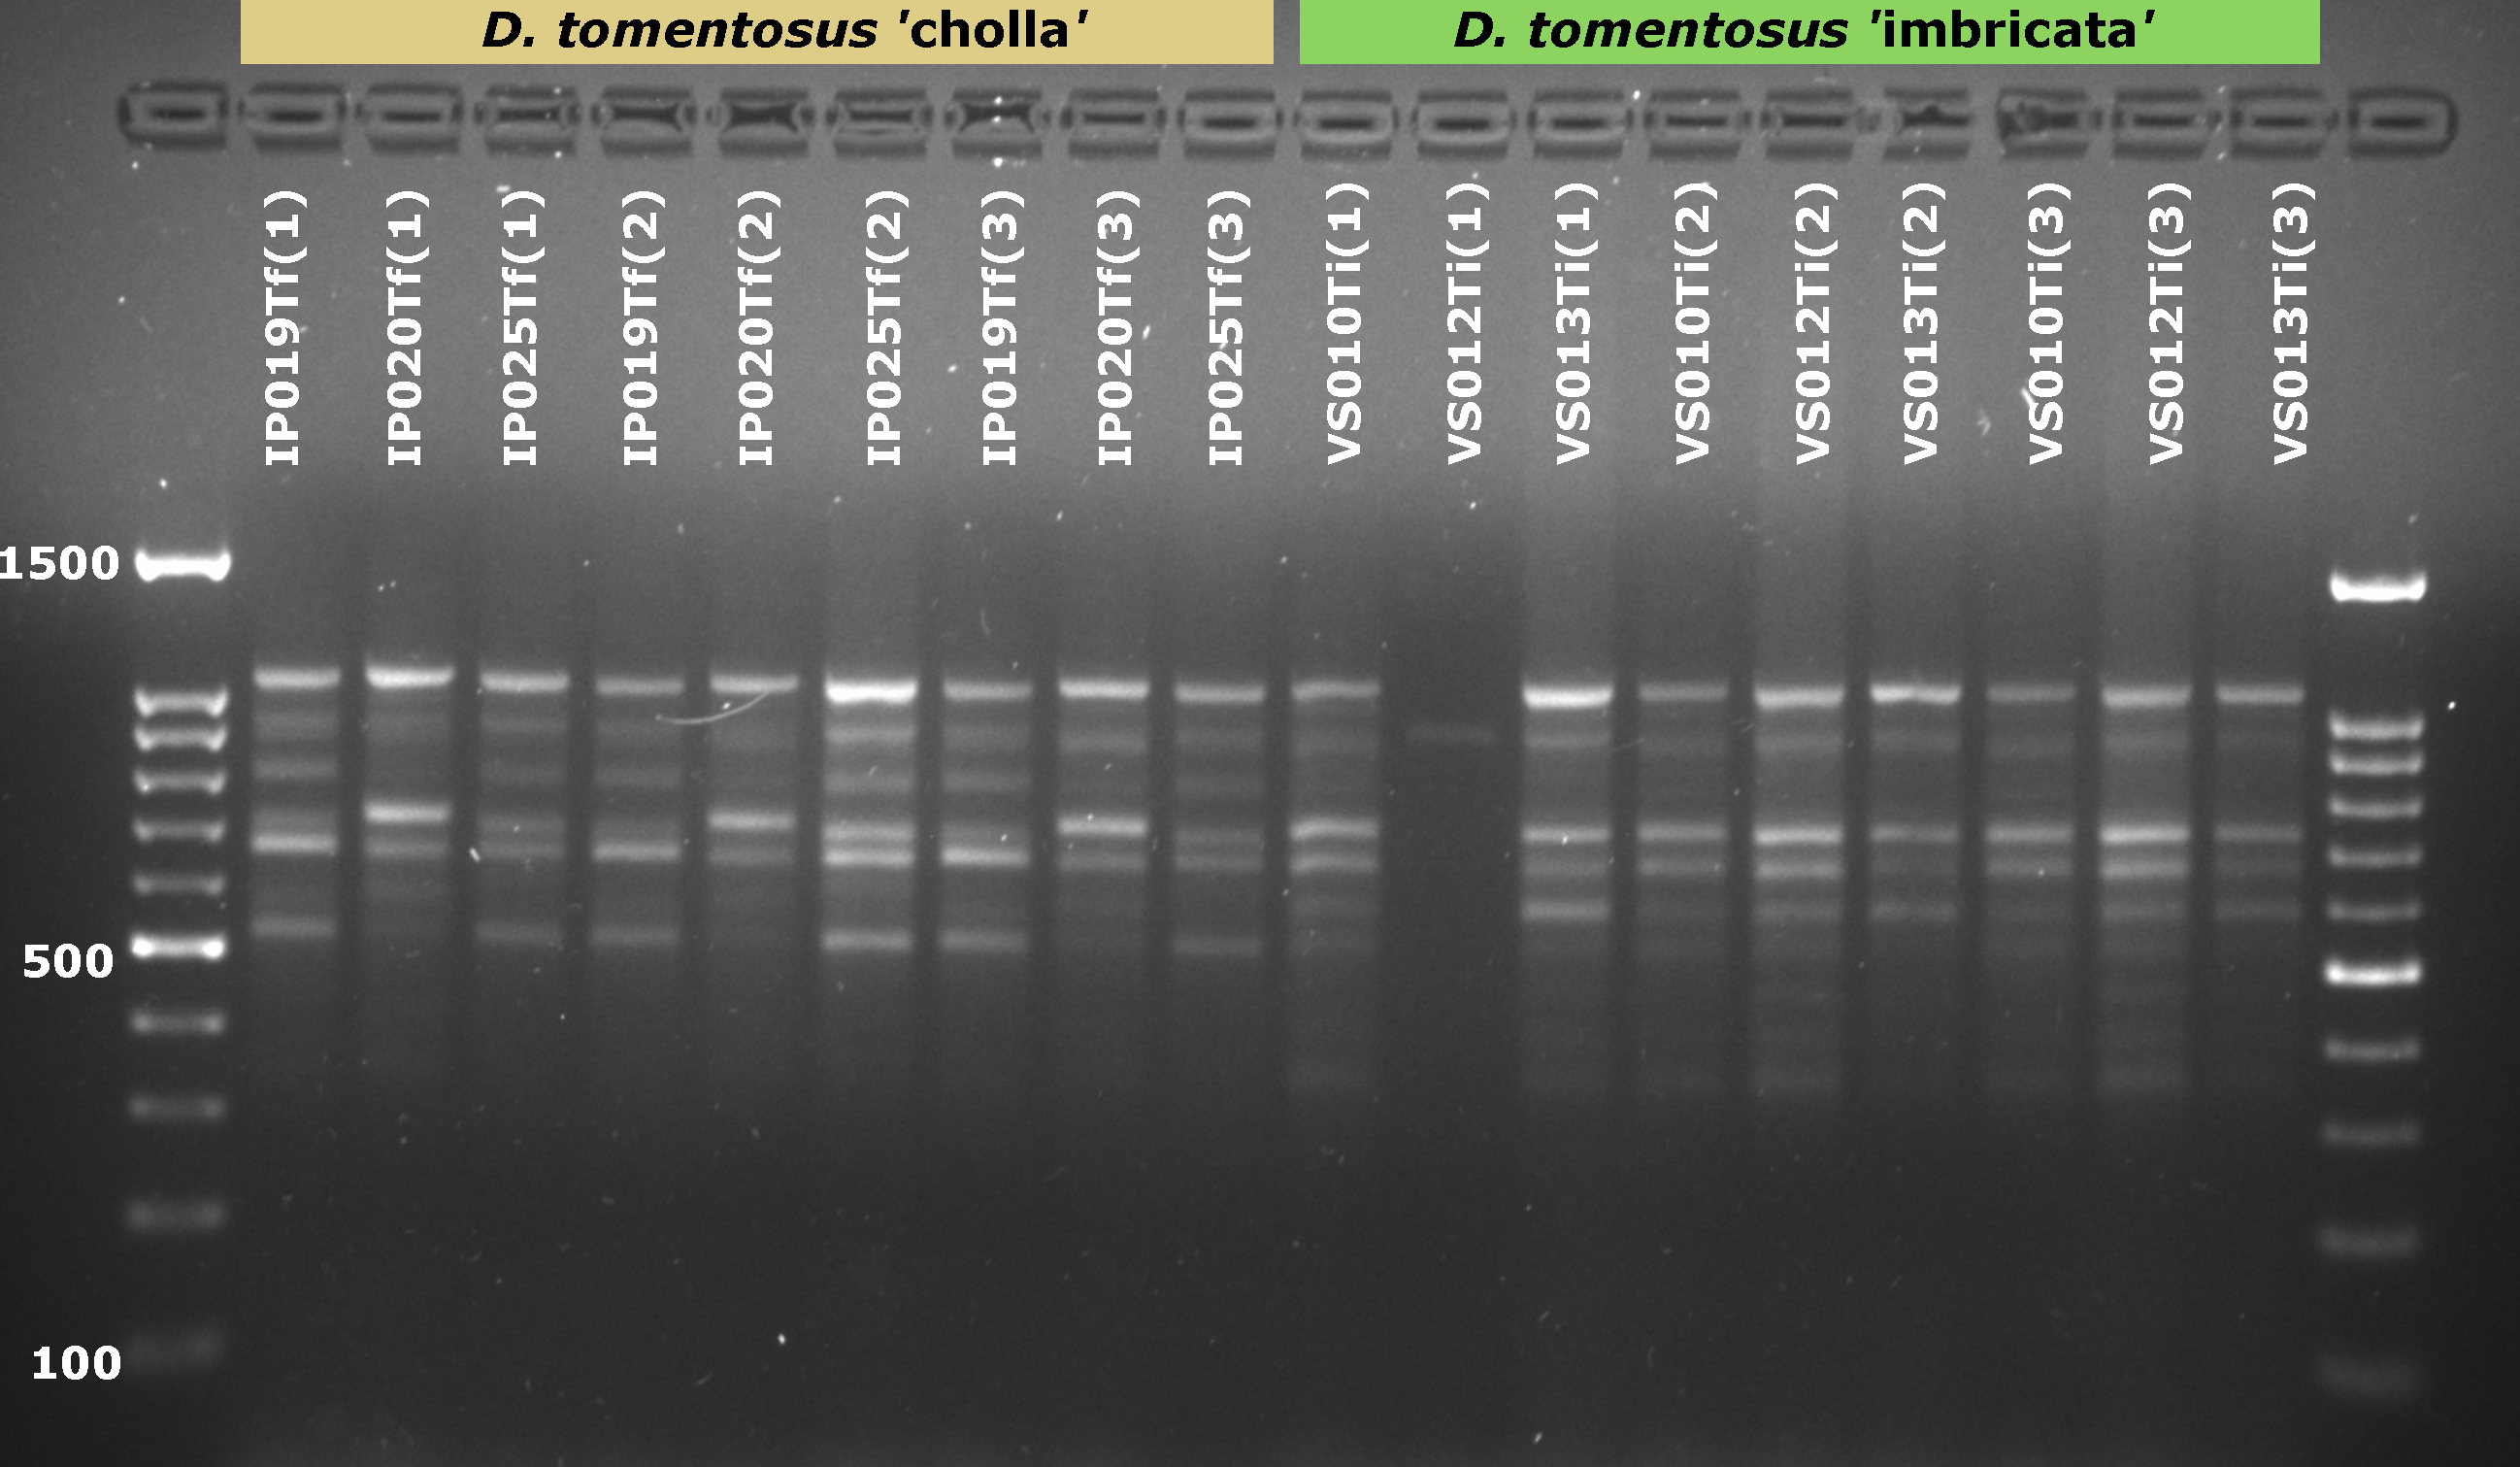
\includegraphics[scale = 0.3]{Images/ISSR_gel_T.pdf}
	\caption{ISSR banding pattern on a 1.5\% agarose gel for the two \textit{D. tomentosus} lineages (`cholla' and `imbricata'), run as a preliminary test before fragment analysis. Ladders are on the far left and right, marked at 100, 500 and 1500 base pair sizes.}
	\label{fig:issrGel}
\end{figure}

\begin{landscape}
{\scriptsize %
\renewcommand{\arraystretch}{0.5}
\begin{longtable}{@{}lllllp{2.7cm}p{2.2cm}p{5cm}p{4cm}@{}}
\caption{Genbank accession numbers for 12S, 18S and COI genetic sequences; with the extraction sample ID, species, lineage, locality and host plant information. CT Bot. Gard. = Cape Town Botanical Gardens, EC = Eastern Cape, KNP = Kruger National Park, MRF = Mass Rearing Facility. Black dots indicate samples collected in the native range in 2017.} \label{appendix:sequenceInfo} \\
\toprule
\textbf{12S} & \textbf{18S} & \textbf{COI DTOMf} & \textbf{COI PcoF1} & \textbf{Extraction ID} & \textbf{Species} & \textbf{Lineage} & \textbf{Locality} & \textbf{Host plant} \\ \midrule
MN220012 &  &  &  & VS021Au & \textit{D. austrinus} &  & South Africa: Uitenhage & \textit{Opuntia aurantiaca} \\
MN220013 & MN310065 &  &  & IP001Au & \textit{D. austrinus} &  & South Africa: Uitenhage & \textit{Opuntia aurantiaca} \\
MN220014 & MN310073 &  &  & VS001Au & \textit{D. austrinus} &  & South Africa: Uitenhage & \textit{Opuntia aurantiaca} \\
MN220038 & MN310132 &  &  & VS022Au & \textit{D. austrinus} &  & South Africa: Uitenhage & \textit{Opuntia aurantiaca} \\
MN220079 &  &  &  & VS089Au & \textit{D. austrinus} &  & South Africa: Uitenhage & \textit{Opuntia aurantiaca} \\
MN220091 & MN310131 &  &  & VS090Au & \textit{D. austrinus} &  & South Africa: Uitenhage & \textit{Opuntia aurantiaca} \\
MN220130 & MN310178 &  &  & Au4 & \textit{D. austrinus} &  & Australia: Queensland & \textit{Opuntia aurantiaca} \\
MN220131 & MN310179 &  &  & Au3 & \textit{D. austrinus} &  & Australia: Queensland & \textit{Opuntia aurantiaca} \\
MN220132 & MN310149 &  &  & Au1 & \textit{D. austrinus} &  & Australia: Queensland & \textit{Opuntia aurantiaca} \\
 & MN310069 &  &  & IP021Au & \textit{D. austrinus} &  & South Africa: Uitenhage & \textit{Opuntia aurantiaca} \\
 & MN310130 &  &  & VS091Au & \textit{D. austrinus} &  & South Africa: Uitenhage & \textit{Opuntia aurantiaca} \\
MN220010 &  &  &  & VS020C & \textit{D. ceylonicus} &  & South Africa: Uitenhage & \textit{Opuntia monacantha} \\
MN220011 & MN310074 &  &  & VS002C & \textit{D. ceylonicus} &  & South Africa: Uitenhage & \textit{Opuntia monacantha} \\
MN220037 & MN310134 &  &  & VS019C & \textit{D. ceylonicus} &  & South Africa: Uitenhage & \textit{Opuntia monacantha} \\
MN220039 & MN310133 &  &  & VS021C & \textit{D. ceylonicus} &  & South Africa: Uitenhage & \textit{Opuntia monacantha} \\
MN220122 & MN310173 &  &  & cey4 & \textit{D. ceylonicus} &  & Australia: Queensland & \textit{Opuntia monacantha} \\
MN220123 & MN310152 &  &  & cey3 & \textit{D. ceylonicus} &  & Australia: Queensland & \textit{Opuntia monacantha} \\
MN220124 & MN310160 &  &  & cey2 & \textit{D. ceylonicus} &  & Australia: Queensland & \textit{Opuntia monacantha} \\
 & MN310070 &  &  & IP022C & \textit{D. ceylonicus} &  & South Africa: Uitenhage & \textit{Opuntia monacantha} \\
 & MN310081 &  &  & VS020C & \textit{D. ceylonicus} &  & South Africa: Uitenhage & \textit{Opuntia monacantha} \\
 & MN310174 &  &  & cey1 & \textit{D. ceylonicus} &  & Australia: Queensland & \textit{Opuntia monacantha} \\
 & MN310037 &  & MN372226 & CSW001H & \textit{D. confertus} &  & Namibia, Windhoek & \textit{Harrisia sp.} \\
 & MN310038 &  & MN372227 & CSW002H & \textit{D. confertus} &  & Namibia, Windhoek & \textit{Harrisia sp.} \\
MN220015 & MN310099 &  & MN372274 & VS100Con\_s & \textit{D. confusus} &  & USA: Arizona, Tucson \textbullet & \textit{Opuntia santa-rita} \\
MN220016 & MN310100 &  &  & VS101Con\_e & \textit{D. confusus} &  & USA: Arizona, Tucson  & \textit{Opuntia engelmannii} \\
MN220017 & MN310101 &  &  & VS102Con\_e & \textit{D. confusus} &  & USA: Arizona, Tucson  & \textit{Opuntia engelmannii} \\
MN220018 & MN310102 &  &  & VS103Con\_e & \textit{D. confusus} &  & USA: Arizona, Tucson  & \textit{Opuntia engelmannii} \\
MN220019 & MN310103 &  &  & VS104Con\_e & \textit{D. confusus} &  & USA: Arizona, Tucson  & \textit{Opuntia engelmannii} \\
MN220029 &  &  & MN372263 & VS035O.4PM  & \textit{D. confusus} &  & USA: Arizona, Four Peaks Mt. \textbullet & \textit{Opuntia engelmannii} \\
MN220030 &  &  & MN372264 & VS036O.4PM  & \textit{D. confusus} &  & USA: Arizona, Four Peaks Mt. \textbullet & \textit{Opuntia engelmannii} \\
MN220031 & MN310091 &  & MN372265 & VS037O.4PM  & \textit{D. confusus} &  & USA: Arizona, Four Peaks Mt. \textbullet & \textit{Opuntia engelmannii} \\
MN220032 & MN310092 &  & MN372266 & VS038O.lc  & \textit{D. confusus} &  & USA: New Mexico, Las Cruces \textbullet & \textit{Opuntia engelmannii} \\
MN220033 & MN310093 &  & MN372267 & VS039O.lc  & \textit{D. confusus} &  & USA: New Mexico, Las Cruces \textbullet & \textit{Opuntia engelmannii} \\
MN220034 & MN310094 &  & MN372268 & VS040O.lc  & \textit{D. confusus} &  & USA: New Mexico, Las Cruces \textbullet & \textit{Opuntia engelmannii} \\
MN220054 & MN310054 &  & MN372240 & VS072u & \textit{D. confusus} &  & USA: Texas, Laredo \textbullet & \textit{Opuntia engelmannii} \\
MN220055 & MN310055 &  & MN372241 & VS073u & \textit{D. confusus} &  & USA: Texas, Laredo \textbullet & \textit{Opuntia engelmannii} \\
MN220056 & MN310056 &  & MN372242 & VS074u & \textit{D. confusus} &  & USA: Texas, Laredo \textbullet & \textit{Opuntia engelmannii} \\
MN220059 & MN310060 &  & MN372246 & VS078u & \textit{D. confusus} &  & USA: Arizona, Tucson \textbullet & \textit{Opuntia engelmannii} \\
MN220060 & MN310063 &  & MN372249 & VS081u & \textit{D. confusus} &  & USA: New Mexico, Las Cruces \textbullet & \textit{Opuntia engelmannii} \\
MN220063 & MN310061 &  & MN372247 & VS079u & \textit{D. confusus} &  & USA: Arizona, Tucson \textbullet & \textit{Opuntia engelmannii} \\
MN220064 & MN310062 &  & MN372248 & VS080u & \textit{D. confusus} &  & USA: New Mexico, Las Cruces \textbullet & \textit{Opuntia engelmannii} \\
 & MN310057 &  & MN372243 & VS075u & \textit{D. confusus} &  & USA: Texas, Laredo \textbullet & \textit{Opuntia engelmannii} \\
MN219994 & MN310078 &  &  & VS015Ofi & \textit{D. opuntiae} & ficus & South Africa: Uitenhage & \textit{Opuntia ficus-indica} \\
MN219995 & MN310079 &  & MN372255 & VS016Ofi & \textit{D. opuntiae} & ficus & South Africa: Uitenhage & \textit{Opuntia ficus-indica} \\
MN219996 & MN310080 &  & MN372256 & VS017Ofi & \textit{D. opuntiae} & ficus & South Africa: Uitenhage & \textit{Opuntia ficus-indica} \\
MN219997 & MN310095 &  & MN372269 & VS044Ofi & \textit{D. opuntiae} & ficus & Namibia: Auros farm & \textit{Opuntia ficus-indica} \\
MN219998 & MN310096 &  & MN372271 & VS046Ofi & \textit{D. opuntiae} & ficus & Namibia: Auros farm & \textit{Opuntia ficus-indica} \\
MN219999 & MN310142 &  & MN372270 & VS045Ofi & \textit{D. opuntiae} & ficus & Namibia: Auros farm & \textit{Opuntia ficus-indica} \\
MN220005 & MN310066 &  &  & IP003Os & \textit{D. opuntiae} &  & South Africa: Uitenhage, MRF & \textit{Opuntia ficus-indica} \\
MN220006 & MN310098 &  & MN372273 & VS054Os & \textit{D. opuntiae} & ficus & Namibia: Auros farm & \textit{Opuntia stricta} \\
MN220007 & MN310139 &  &  & VS055Os & \textit{D. opuntiae} & ficus & Namibia: Auros farm & \textit{Opuntia stricta} \\
MN220008 & MN310097 &  & MN372272 & VS053Os & \textit{D. opuntiae} & ficus & Namibia: Auros farm & \textit{Opuntia stricta} \\
MN220009 & MN310075 &  & MN372252 & VS004Os & \textit{D. opuntiae} &  & South Africa: Uitenhage, MRF & \textit{Opuntia ficus-indica} \\
MN220020 & MN310082 &  & MN372257 & VS026O.flag & \textit{D. opuntiae} &  & USA: Arizona, Flagstaff \textbullet & \textit{Opuntia engelmannii} \\
MN220021 & MN310083 &  & MN372258 & VS027O.flag & \textit{D. opuntiae} &  & USA: Arizona, Flagstaff \textbullet & \textit{Opuntia engelmannii} \\
MN220022 & MN310084 &  &  & VS028O.flag & \textit{D. opuntiae} &  & USA: Arizona, Flagstaff \textbullet & \textit{Opuntia engelmannii} \\
MN220023 & MN310085 &  &  & VS029O.tuc & \textit{D. opuntiae} &  & USA: Arizona, Tucson \textbullet & \textit{Opuntia engelmannii} \\
MN220024 & MN310086 &  & MN372259 & VS030O.tuc & \textit{D. opuntiae} &  & USA: Arizona, Tucson \textbullet & \textit{Opuntia engelmannii} \\
MN220025 & MN310087 &  & MN372260 & VS031O.tuc & \textit{D. opuntiae} &  & USA: Arizona, Tucson \textbullet & \textit{Opuntia engelmannii} \\
MN220026 & MN310088 &  & MN372261 & VS032O.sed & \textit{D. opuntiae} &  & USA: Arizona, Sedona \textbullet & \textit{Opuntia engelmannii} \\
MN220027 & MN310089 &  &  & VS033O.sed & \textit{D. opuntiae} &  & USA: Arizona, Sedona \textbullet & \textit{Opuntia engelmannii} \\
MN220028 & MN310090 &  & MN372262 & VS034O.sed & \textit{D. opuntiae} &  & USA: Arizona, Sedona \textbullet & \textit{Opuntia engelmannii} \\
MN220035 & MN310039 &  & MN372228 & CSW003E & \textit{D. opuntiae} & ficus & Namibia, Windhoek & \textit{Opuntia engelmannii} \\
MN220036 & MN310040 &  &  & CSW004E & \textit{D. opuntiae} & ficus & Namibia, Windhoek & \textit{Opuntia engelmannii} \\
MN220043 & MN310041 &  & MN372229 & VS059Os & \textit{D. opuntiae} &  & South Africa: Uitenhage, MRF & \textit{Opuntia ficus-indica} \\
MN220044 & MN310042 &  & MN372230 & VS060Os & \textit{D. opuntiae} &  & South Africa: Uitenhage, MRF & \textit{Opuntia ficus-indica} \\
MN220045 & MN310043 &  & MN372231 & VS061Os & \textit{D. opuntiae} &  & South Africa: Uitenhage, MRF & \textit{Opuntia ficus-indica} \\
MN220046 & MN310044 &  & MN372232 & VS062Os & \textit{D. opuntiae} &  & South Africa: Uitenhage, MRF & \textit{Opuntia ficus-indica} \\
MN220047 & MN310045 &  & MN372233 & VS063Os & \textit{D. opuntiae} &  & South Africa: Uitenhage, MRF & \textit{Opuntia ficus-indica} \\
MN220048 & MN310046 &  & MN372234 & VS064u & \textit{D. opuntiae} &  & USA: Texas, Moor Airbase \textbullet & \textit{Opuntia engelmannii} \\
MN220049 & MN310047 &  & MN372235 & VS065u & \textit{D. opuntiae} &  & USA: Texas, Moor Airbase \textbullet & \textit{Opuntia engelmannii} \\
MN220050 & MN310048 &  & MN372236 & VS066u & \textit{D. opuntiae} &  & USA: Texas, Port Isabel \textbullet & \textit{Opuntia engelmannii} \\
MN220051 & MN310050 &  & MN372238 & VS068u & \textit{D. opuntiae} &  & USA: Texas, Laredo \textbullet & \textit{Opuntia engelmannii} \\
MN220052 & MN310051 &  &  & VS069u & \textit{D. opuntiae} &  & USA: Texas, Laredo \textbullet & \textit{Opuntia engelmannii} \\
MN220053 & MN310053 &  & MN372239 & VS071u & \textit{D. opuntiae} &  & USA: Texas, Webb \textbullet & \textit{Opuntia engelmannii} \\
MN220057 & MN310058 &  & MN372244 & VS076u & \textit{D. opuntiae} &  & USA: California, Rincon \textbullet & \textit{Opuntia engelmannii} \\
MN220058 & MN310059 &  & MN372245 & VS077u & \textit{D. opuntiae} &  & USA: California, Rincon \textbullet & \textit{Opuntia engelmannii} \\
MN220061 &  &  &  & VS083u & \textit{D. opuntiae} &  & USA: Texas, Pecos County \textbullet & \textit{Opuntia engelmannii} \\
MN220062 & MN310052 &  &  & VS070u & \textit{D. opuntiae} &  & USA: Texas, Webb \textbullet & \textit{Opuntia engelmannii} \\
MN220065 & MN310104 &  &  & VS086uOE & \textit{D. opuntiae} & ficus & South Africa: Cookhouse, EC & \textit{Opuntia engelmannii} \\
MN220066 & MN310116 &  &  & VS087uOE & \textit{D. opuntiae} & ficus & South Africa: Cookhouse, EC & \textit{Opuntia engelmannii} \\
MN220067 & MN310115 &  &  & VS088uOE & \textit{D. opuntiae} & ficus & South Africa: Cookhouse, EC & \textit{Opuntia engelmannii} \\
MN220074 & MN310107 &  &  & VS106V & \textit{D. opuntiae} & ficus & South Africa: EC & \textit{Opuntia engelmannii} \\
MN220075 & MN310106 &  &  & VS107V & \textit{D. opuntiae} & ficus & South Africa: EC & \textit{Opuntia engelmannii} \\
MN220076 & MN310105 &  &  & VS108V & \textit{D. opuntiae} & ficus & South Africa: EC & \textit{Opuntia engelmannii} \\
MN220077 & MN310125 &  &  & P2S4 & \textit{D. opuntiae} & stricta & South Africa: KNP & \textit{Opuntia stricta} \\
MN220078 & MN310122 &  & MN372278 & P3S2 & \textit{D. opuntiae} & stricta & South Africa: KNP & \textit{Opuntia stricta} \\
MN220080 & MN310145 &  &  & BCCS1 & \textit{D. opuntiae} & stricta & South Africa: KNP, Skukuza & \textit{Opuntia stricta} \\
MN220081 & MN310127 &  & MN372275 & P1S4 & \textit{D. opuntiae} & stricta & South Africa: KNP & \textit{Opuntia stricta} \\
MN220082 &  &  &  & VS054Os & \textit{D. opuntiae} & ficus & South Africa: Namibia & \textit{Opuntia stricta} \\
MN220083 & MN310123 &  &  & P3S1 & \textit{D. opuntiae} & stricta & South Africa: KNP & \textit{Opuntia stricta} \\
MN220084 & MN310128 &  & MN372279 & P1S3 & \textit{D. opuntiae} & stricta & South Africa: KNP & \textit{Opuntia stricta} \\
MN220085 & MN310119 &  & MN372277 & VS151H & \textit{D. opuntiae} & stricta & South Africa & \textit{Opuntia stricta} \\
MN220086 & MN310143 &  & MN372280 & BCCS4 & \textit{D. opuntiae} & stricta & South Africa: KNP, Skukuza & \textit{Opuntia stricta} \\
MN220087 & MN310124 &  &  & P2S5 & \textit{D. opuntiae} & stricta & South Africa: KNP & \textit{Opuntia stricta} \\
MN220088 & MN310129 &  &  & P1S1 & \textit{D. opuntiae} & stricta & South Africa: KNP & \textit{Opuntia stricta} \\
MN220089 & MN310121 &  &  & VS149K & \textit{D. opuntiae} & stricta & South Africa & \textit{Opuntia stricta} \\
MN220090 & MN310144 &  &  & BCCS2 & \textit{D. opuntiae} & stricta & South Africa: KNP, Skukuza & \textit{Opuntia stricta} \\
MN220092 &  &  &  & VS146K & \textit{D. opuntiae} & stricta & South Africa & \textit{Opuntia stricta} \\
MN220093 & MN310126 &  &  & P2S2 & \textit{D. opuntiae} & stricta & South Africa: KNP & \textit{Opuntia stricta} \\
MN220094 & MN310118 &  & MN372276 & VS152H & \textit{D. opuntiae} & stricta & South Africa & \textit{Opuntia stricta} \\
MN220095 & MN310117 &  &  & VS154H & \textit{D. opuntiae} & stricta & South Africa & \textit{Opuntia stricta} \\
MN220096 &  &  &  & Ah2 & \textit{D. opuntiae} & stricta & Saudi Arabia: Jazan, Alaredah & \textit{Opuntia stricta} \\
MN220097 & MN310163 &  &  & op4 & \textit{D. opuntiae} &  & Australia: Queensland & \textit{Opuntia stricta} \\
MN220098 & MN310147 &  &  & op3 & \textit{D. opuntiae} &  & Australia: Queensland & \textit{Opuntia stricta} \\
MN220099 & MN310162 &  &  & op1 & \textit{D. opuntiae} &  & Australia: Queensland & \textit{Opuntia stricta} \\
MN220100 &  &  &  & JC3 & \textit{D. opuntiae} & stricta & Saudi Arabia: Jazan, Jazan City & \textit{Opuntia stricta} \\
MN220101 &  &  &  & JC2 & \textit{D. opuntiae} & stricta & Saudi Arabia: Jazan, Jazan City & \textit{Opuntia stricta} \\
MN220106 &  &  &  & H4 & \textit{D. opuntiae} & stricta & Saudi Arabia: Jazan, Hurob & \textit{Opuntia stricta} \\
MN220107 &  &  &  & H1 & \textit{D. opuntiae} & stricta & Saudi Arabia: Jazan, Hurob & \textit{Opuntia stricta} \\
MN220108 & MN310155 &  &  & eng1 & \textit{D. opuntiae} &  & Australia: Queensland & \textit{Opuntia engelmannii} \\
MN220111 & MN310166 &  &  & eng4 & \textit{D. opuntiae} &  & Australia: Queensland & \textit{Opuntia engelmannii} \\
MN220133 &  &  &  & AL3 & \textit{D. opuntiae} & stricta & Saudi Arabia: Jazan, Aldyer & \textit{Opuntia stricta} \\
MN220134 &  &  &  & AL2 & \textit{D. opuntiae} & stricta & Saudi Arabia: Jazan, Aldyer & \textit{Opuntia stricta} \\
MN220135 &  &  &  & Ah4 & \textit{D. opuntiae} & stricta & Saudi Arabia: Jazan, Alaredah & \textit{Opuntia stricta} \\
 & MN310049 &  & MN372237 & VS067u & \textit{D. opuntiae} &  & USA: Texas, Port Isabel & \textit{Opuntia engelmannii} \\
 & MN310064 &  & MN372250 & VS082u & \textit{D. opuntiae} &  & USA: Texas, Pecos County & \textit{Opuntia engelmannii} \\
 & MN310071 &  &  & IP024Os & \textit{D. opuntiae} &  & South Africa: Uitenhage, MRF & \textit{Opuntia ficus-indica} \\
 & MN310120 &  &  & VS150K & \textit{D. opuntiae} & stricta & South Africa & \textit{Opuntia stricta} \\
 & MN310140 &  &  & CVS262 & \textit{D. opuntiae} & ficus & South Africa: Uitenhage & \textit{Opuntia stricta} \\
 & MN310141 &  &  & CVS261 & \textit{D. opuntiae} & ficus & South Africa: Uitenhage & \textit{Opuntia stricta} \\
 & MN310167 &  &  & eng3 & \textit{D. opuntiae} &  & Australia: Queensland & \textit{Opuntia engelmannii} \\
 &  &  & MN372253 & VS008Ofi & \textit{D. opuntiae} & ficus & South Africa: Uitenhage & \textit{Opuntia ficus-indica} \\
MN220000 & MN310137 &  &  & VS014Ti & \textit{D. tomentosus} & imbricata & South Africa: Uitenhage & \textit{Cylindropuntia imbricata} \\
MN220001 & MN310077 &  &  & VS013Ti & \textit{D. tomentosus} & imbricata & South Africa: Uitenhage & \textit{Cylindropuntia imbricata} \\
MN220002 & MN310076 &  & MN372254 & VS012Ti & \textit{D. tomentosus} & imbricata & South Africa: Uitenhage & \textit{Cylindropuntia imbricata} \\
MN220102 & MN310164 &  &  & imb4 & \textit{D. tomentosus} & imbricata & Australia: Queensland & \textit{Cylindropuntia imbricata} \\
MN220103 & MN310165 &  &  & imb3 & \textit{D. tomentosus} & imbricata & Australia: Queensland & \textit{Cylindropuntia imbricata} \\
MN220104 & MN310156 &  &  & imb2 & \textit{D. tomentosus} & imbricata & Australia: Queensland & \textit{Cylindropuntia imbricata} \\
MN220105 & MN310148 &  &  & imb1 & \textit{D. tomentosus} & imbricata & Australia: Queensland & \textit{Cylindropuntia imbricata} \\
 &  &  & MN372299 & IP005Ti & \textit{D. tomentosus} & imbricata & South Africa: Uitenhage & \textit{Cylindropuntia imbricata} \\
MN220041 & MN310138 &  &  & VS010Ti & \textit{D. tomentosus} & imbricata & South Africa: Uitenhage & \textit{Cylindropuntia imbricata} \\
MN220042 & MN310136 &  &  & IP016Ti & \textit{D. tomentosus} & imbricata & South Africa: Uitenhage & \textit{Cylindropuntia imbricata} \\
MN220003 & MN310072 &  & MN372251 & IP025Tf & \textit{D. tomentosus} & cholla & South Africa: CT Bot. Gard. & \textit{C. fulgida var. mamm.} \\
MN220004 & MN310135 &  &  & VS005Tf & \textit{D. tomentosus} & cholla & South Africa: CT Bot. Gard. & \textit{C. fulgida var. mamm.} \\
MN220040 & MN310068 & MN372298 &  & IP019Tf & \textit{D. tomentosus} & cholla & South Africa: CT Bot. Gard. & \textit{C. fulgida var. mamm.} \\
MN220068 & MN310114 &  &  & VS098Tf & \textit{D. tomentosus} & cholla & South Africa: CT Bot. Gard. & \textit{C. fulgida var. mamm.} \\
MN220069 & MN310113 &  &  & VS099Tf & \textit{D. tomentosus} & cholla & South Africa: CT Bot. Gard. & \textit{C. fulgida var. mamm.} \\
MN220109 &  &  &  & Ekh6 & \textit{D. tomentosus} & cholla & South Africa: Jansenville, EC & \textit{Cylindropuntia fulgida} \\
MN220110 &  &  &  & EKh5 & \textit{D. tomentosus} & cholla & South Africa: Jansenville, EC & \textit{Cylindropuntia fulgida} \\
MN220112 &  &  &  & Ekh4 & \textit{D. tomentosus} & cholla & South Africa: Jansenville, EC & \textit{Cylindropuntia fulgida} \\
MN220119 &  & MN372287 &  & chol4 & \textit{D. tomentosus} & cholla & Australia: Queensland & \textit{Cylindropuntia fulgida} \\
MN220120 & MN310153 & MN372288 &  & chol3 & \textit{D. tomentosus} & cholla & Australia: Queensland & \textit{Cylindropuntia fulgida} \\
MN220121 & MN310172 & MN372290 &  & chol1 & \textit{D. tomentosus} & cholla & Australia: Queensland & \textit{Cylindropuntia fulgida} \\
 & MN310161 & MN372289 &  & chol2 & \textit{D. tomentosus} & cholla & Australia: Queensland & \textit{C. fulgida var. mamm.} \\
 & MN310067 &  &  & IP005Tf & \textit{D. tomentosus} & cholla & South Africa: CT Bot. Gard. & \textit{C. fulgida var. mamm.} \\
MN220070 & MN310112 &  &  & VS101Tp & \textit{D. tomentosus} & californica & Australia: Queensland & \textit{Cylindropuntia pallida} \\
MN220071 & MN310111 &  &  & VS102Tp & \textit{D. tomentosus} & californica & Australia: Queensland & \textit{Cylindropuntia pallida} \\
MN220072 & MN310109 &  &  & VS104Tp & \textit{D. tomentosus} & californica & Australia: Queensland & \textit{Cylindropuntia pallida} \\
MN220073 & MN310108 &  &  & VS105Tp & \textit{D. tomentosus} & californica & Australia: Queensland & \textit{Cylindropuntia pallida} \\
MN220125 & MN310175 & MN372291 &  & Cal4 & \textit{D. tomentosus} & californica & Australia: Queensland & \textit{Cylindropuntia pallida} \\
MN220126 & MN310151 & MN372292 &  & Cal3 & \textit{D. tomentosus} & californica & Australia: Queensland & \textit{Cylindropuntia pallida} \\
MN220127 & MN310158 & MN372293 &  & Cal2 & \textit{D. tomentosus} & californica & Australia: Queensland & \textit{Cylindropuntia pallida} \\
MN220128 & MN310176 & MN372294 &  & Cal1 & \textit{D. tomentosus} & californica & Australia: Queensland & \textit{Cylindropuntia pallida} \\
 & MN310110 &  &  & VS103Tp & \textit{D. tomentosus} & californica & Australia: Queensland & \textit{Cylindropuntia pallida} \\
MN220113 & MN310146 & MN372281 &  & ech4 & \textit{D. tomentosus} & ech. x acanth. & Australia: Queensland & \textit{\begin{tabular}[c]{@{}l@{}}C. ech. x  C. acanth.\end{tabular}} \\
MN220114 & MN310168 & MN372282 &  & ech3 & \textit{D. tomentosus} & ech. x acanth. & Australia: Queensland & \textit{\begin{tabular}[c]{@{}l@{}}C. ech. x C. acanth.\end{tabular}} \\
MN220115 &  & MN372283 &  & ech2 & \textit{D. tomentosus} & ech. x acanth. & Australia: Queensland & \textit{\begin{tabular}[c]{@{}l@{}}C. ech. x C. acanth.\end{tabular}} \\
MN220118 & MN310169 & MN372284 &  & ech1 & \textit{D. tomentosus} & ech. x acanth. & Australia: Queensland & \textit{\begin{tabular}[c]{@{}l@{}}C. ech. x C. acanth.\end{tabular}} \\
MN220116 & MN310157 & MN372285 &  & cyl3 & \textit{D. tomentosus} & cylindropuntia & Australia: Queensland & \textit{Cylindropuntia sp.} \\
MN220117 & MN310170 & MN372286 &  & cyl2 & \textit{D. tomentosus} & cylindropuntia & Australia: Queensland & \textit{Cylindropuntia sp.} \\
 & MN310154 &  &  & cyl4 & \textit{D. tomentosus} & cylindropuntia & Australia: Queensland & \textit{Cylindropuntia sp.} \\
 & MN310171 &  &  & cyl1 & \textit{D. tomentosus} & cylindropuntia & Australia: Queensland & \textit{Cylindropuntia sp.} \\
MN220129 & MN310159 & MN372297 &  & Big2 & \textit{D. tomentosus} & bigelovii & Australia: Queensland & \textit{Cylindropuntia bigelovii} \\
 & MN310150 & MN372296 &  & Big3 & \textit{D. tomentosus} & bigelovii & Australia: Queensland & \textit{Cylindropuntia bigelovii} \\
 & MN310177 & MN372295 &  & Big5 & \textit{D. tomentosus} & bigelovii & Australia: Queensland & \textit{Cylindropuntia bigelovii} \\ \bottomrule
\end{longtable}
}%


\begin{table}[H]
\centering
\caption{Sample IDs for additional DNA extractions used for ISSR analyses.}
\label{appendix:issr_sample_table}
{\scriptsize %
\renewcommand{\arraystretch}{0.5}
\begin{tabular}{@{}lllll@{}}
\toprule
\textbf{Extraction ID} & \textbf{Species} & \textbf{Lineage} & \textbf{Locality} & \textbf{Host plant} \\ \midrule
VS121O.4PM & \textit{D. confusus} &  & USA: Arizona, Four Peaks Mt. & \textit{O. engelmannii} \\
VS124O.lc & \textit{D. confusus} &  & USA: New Mexico, Las Cruces & \textit{O. engelmannii} \\
VS136 & \textit{D. confusus} &  & USA: Texas, Laredo & \textit{O. engelmannii} \\
VS137 & \textit{D. confusus} &  & USA: Texas, Laredo & \textit{O. engelmannii} \\
VS138 & \textit{D. confusus} &  & USA: Texas, Laredo & \textit{O. engelmannii} \\
VS139 & \textit{D. confusus} &  & USA: Texas, Laredo & \textit{O. engelmannii} \\
VS141 & \textit{D. confusus} &  & USA: Arizona, Tucson & \textit{O. engelmannii} \\
VS142 & \textit{D. confusus} &  & USA: Arizona, Tucson & \textit{O. engelmannii} \\
VS143 & \textit{D. confusus} &  & USA: New Mexico, Las Cruces & \textit{O. engelmannii} \\
VS144 & \textit{D. confusus} &  & USA: New Mexico, Las Cruces & \textit{O. engelmannii} \\
VS110 & \textit{D. opuntiae} & `ficus' & South Africa: EC, Prieel, near Fort Beaufort & \textit{O. ficus-indica} \\
VS111 & \textit{D. opuntiae} & `ficus' & South Africa: EC, Prieel, near Fort Beaufort & \textit{O. ficus-indica} \\
VS112 & \textit{D. opuntiae} & `ficus' & South Africa: EC, Prieel, near Fort Beaufort & \textit{O. ficus-indica} \\
VS113 & \textit{D. opuntiae} & `ficus' & South Africa: EC, Prieel, near Fort Beaufort & \textit{O. engelmannii} \\
VS114 & \textit{D. opuntiae} & `ficus' & South Africa: EC, Prieel, near Fort Beaufort & \textit{O. engelmannii} \\
VS115 & \textit{D. opuntiae} & `ficus' & South Africa: EC, Prieel, near Fort Beaufort & \textit{O. engelmannii} \\
VS116 & \textit{D. opuntiae} & `ficus' & South Africa: EC, Kluklu farm, near Fort Beaufort & \textit{O. engelmannii} \\
VS117 & \textit{D. opuntiae} & `ficus' & South Africa: EC, Kluklu farm, near Fort Beaufort & \textit{O. engelmannii} \\
VS118 & \textit{D. opuntiae} & `ficus' & South Africa: EC, Kluklu farm, near Fort Beaufort & \textit{O. engelmannii} \\
VS119O.flag & \textit{D. opuntiae} &  & USA: Arizona, Flagstaff & \textit{O. engelmannii} \\
VS120O.flag & \textit{D. opuntiae} &  & USA: Arizona, Flagstaff & \textit{O. engelmannii} \\
VS126O.sed & \textit{D. opuntiae} &  & USA: Arizona, Sedona & \textit{O. engelmannii} \\
VS129 & \textit{D. opuntiae} &  & USA: Texas, Moor Airbase & \textit{O. engelmannii} \\
VS130 & \textit{D. opuntiae} &  & USA: Texas, Port Isabel & \textit{O. engelmannii} \\
VS131 & \textit{D. opuntiae} &  & USA: Texas, Port Isabel & \textit{O. engelmannii} \\
VS132 & \textit{D. opuntiae} &  & USA: Texas, Laredo & \textit{O. engelmannii} \\
VS133 & \textit{D. opuntiae} &  & USA: Texas, Laredo & \textit{O. engelmannii} \\
VS134 & \textit{D. opuntiae} &  & USA: Texas, Webb & \textit{O. engelmannii} \\
VS135 & \textit{D. opuntiae} &  & USA: Texas, Webb & \textit{O. engelmannii} \\
VS140 & \textit{D. opuntiae} &  & USA: California, Rincon & \textit{O. engelmannii} \\
VS145 & \textit{D. opuntiae} &  & USA: Texas, Pecos County & \textit{O. engelmannii} \\
VS092Ti & \textit{D. tomentosus} & `imbricata' & South Africa: Uitenhage MRF & \textit{C. imbricata} \\
VS093Ti & \textit{D. tomentosus} & `imbricata' & South Africa: Uitenhage MRF & \textit{C. imbricata} \\
VS100Tf & \textit{D. tomentosus} & `cholla' & South Africa: Uitenhage MRF & \textit{C. fulgida} var. \textit{mamillata} \\ \bottomrule
\end{tabular}
}%
\end{table}


\begin{table}[H]
\caption{Genbank sequences used to supplement the dataset for this project. PcoF1 \& LepR1 and DTOMf \& HCO2198 are both COI primers that amplify the same region of the COI gene.} \label{appendix:outgroups}
\centering
{\scriptsize %
\renewcommand{\arraystretch}{0.4}
\begin{tabular}{@{}lllll@{}} \\ \toprule
\multicolumn{4}{c}{\textbf{Genbank accession numbers}} & \multicolumn{1}{c}{\textbf{Organism}}  \\ \toprule
\multicolumn{1}{c}{\textbf{12S}} & \textbf{18S} & \textbf{PcoF1 \& LepR1} & \textbf{DTOMf \& HCO2198} &  \\ \bottomrule
HQ893819.1 & KY9276001 &  &  & \textit{Parasaissetia nigra} \\
HQ893810.1 & HQ8937881 &  &  & \textit{Ceroplastes sinensis} \\
HQ893818.1 & HQ8937931 & GU936953.1 &  & \textit{Coccus viridis} \\
KT199030.1 & KT199030.1 &  &  & \textit{Marchalina hellenica} \\
HQ893806.1 & KT199034.1 & KP692469.1 &  & \textit{Icerya purchasi} \\
KJ701959.1 & KJ7019951 &  &  & \textit{Dactylopius coccus} \\
KJ701960.1 & KJ7019941 &  &  & \textit{Dactylopius coccus} \\
KJ701961.1 & KJ7019931 &  &  & \textit{Dactylopius coccus} \\
KJ701962.1 & KJ7019921 &  &  & \textit{Dactylopius coccus} \\
KJ701963.1 & KJ7019911 &  &  & \textit{Dactylopius coccus} \\
 &  &  &  & \textit{Ceroplastes sp.} \\
 &  &  & GU228789.1 & \textit{Dactylopius opuntiae} \\
 &  &  & GU228788.1 & \textit{Dactylopius tomentosus 'Imbricata'} \\
 &  &  & GU228787.1 & \textit{Dactylopius tomentosus 'Imbricata'} \\
 &  &  & GU228786.1 & \textit{Dactylopius tomentosus 'RoseaP'} \\
 &  &  & GU228781.1 & \textit{Dactylopius tomentosus 'ChollaDH'} \\
 &  &  & GU228780.1 & \textit{Dactylopius tomentosus 'ChollaE'} \\
 &  &  & GU228779.1 & \textit{Dactylopius tomentosus 'ChollaD'} \\
 &  &  & GU228785.1 & \textit{Dactylopius tomentosus 'RoseaY'} \\
 &  &  & GU228784.1 & \textit{Dactylopius tomentosus 'Fulgida'} \\
 &  &  & GU228783.1 & \textit{Dactylopius tomentosus 'Mamillata'} \\
 &  &  & GU228782.1 & \textit{Dactylopius tomentosus 'Molesta'} \\
 &  &  & AB440069.2 & \textit{Coccus hesperidum} \\
 &  &  & AB440071.1 & \textit{Eulecanium kunoense} \\
 &  &  & AB440073.1 & \textit{Parthenolecanium pruinosum} \\
 &  &  & AB440072.2 & \textit{Pulvinaria psidii} \\ \bottomrule
\end{tabular}
}%
\end{table}

% Please add the following required packages to your document preamble:
% \usepackage{booktabs}
\begin{table}[H]
\caption{Rhodes University and Agricultural Research Council (ARC) accession numbers for \textit{Dactylopius} samples from the native range (USA), identified by Ian Millar in 2019. Representative sample IDs refer to those used in the gene phylogenies in this project. See Table \ref{appendix:sequenceInfo} for the full list of sequences.} \label{appendix:ianMillarIds}
\centering
{\scriptsize %
\renewcommand{\arraystretch}{0.4}
\begin{tabular}{@{}llll@{}}
\toprule
\textbf{\begin{tabular}[c]{@{}l@{}}Rhodes University \\ Accession Number\end{tabular}} & \textbf{\begin{tabular}[c]{@{}l@{}}ARC \\ Accession Number\end{tabular}} & \textbf{Identity} & \textbf{\begin{tabular}[c]{@{}l@{}}Representative \\ sample ID\end{tabular}} \\ \midrule
RH1283 & HC 7331 & \textit{D. confertus} & \multirow{3}{*}{CSW001H} \\
RH1284 & HC 7331 & \textit{D. confertus} &  \\
RH1285 & HC 7331 & \textit{D. confertus} &  \\
RH1286 & HC 7332 & \textit{D. confusus} & VS072u \\
RH1287 & HC 7333 & \textit{D. opuntiae} & VS083u \\
RH1288 & HC 7334 & \textit{D. opuntiae} & VS069u \\
RH1289 &  & \textit{D. confusus} & VS080u \\
RH1290 & HC 7335 & \textit{D. opuntiae} & VS064u \\
RH1291 & HC 7336 & \textit{D. opuntiae} & VS077u \\
RH1292 & HC 7337 & \textit{D. opuntiae} & VS083u \\
RH1293 & HC 7338 & \textit{D. confusus} & VS073u \\
RH1294 &  & \textit{D. confusus} & VS078u \\
RH1295 &  & \textit{D. opuntiae} & VS066u \\ \bottomrule
\end{tabular}
}%
\end{table}

\end{landscape}


\begin{landscape}
\label{sec:tcoffee}

\begin{figure}[H]
	\centering
	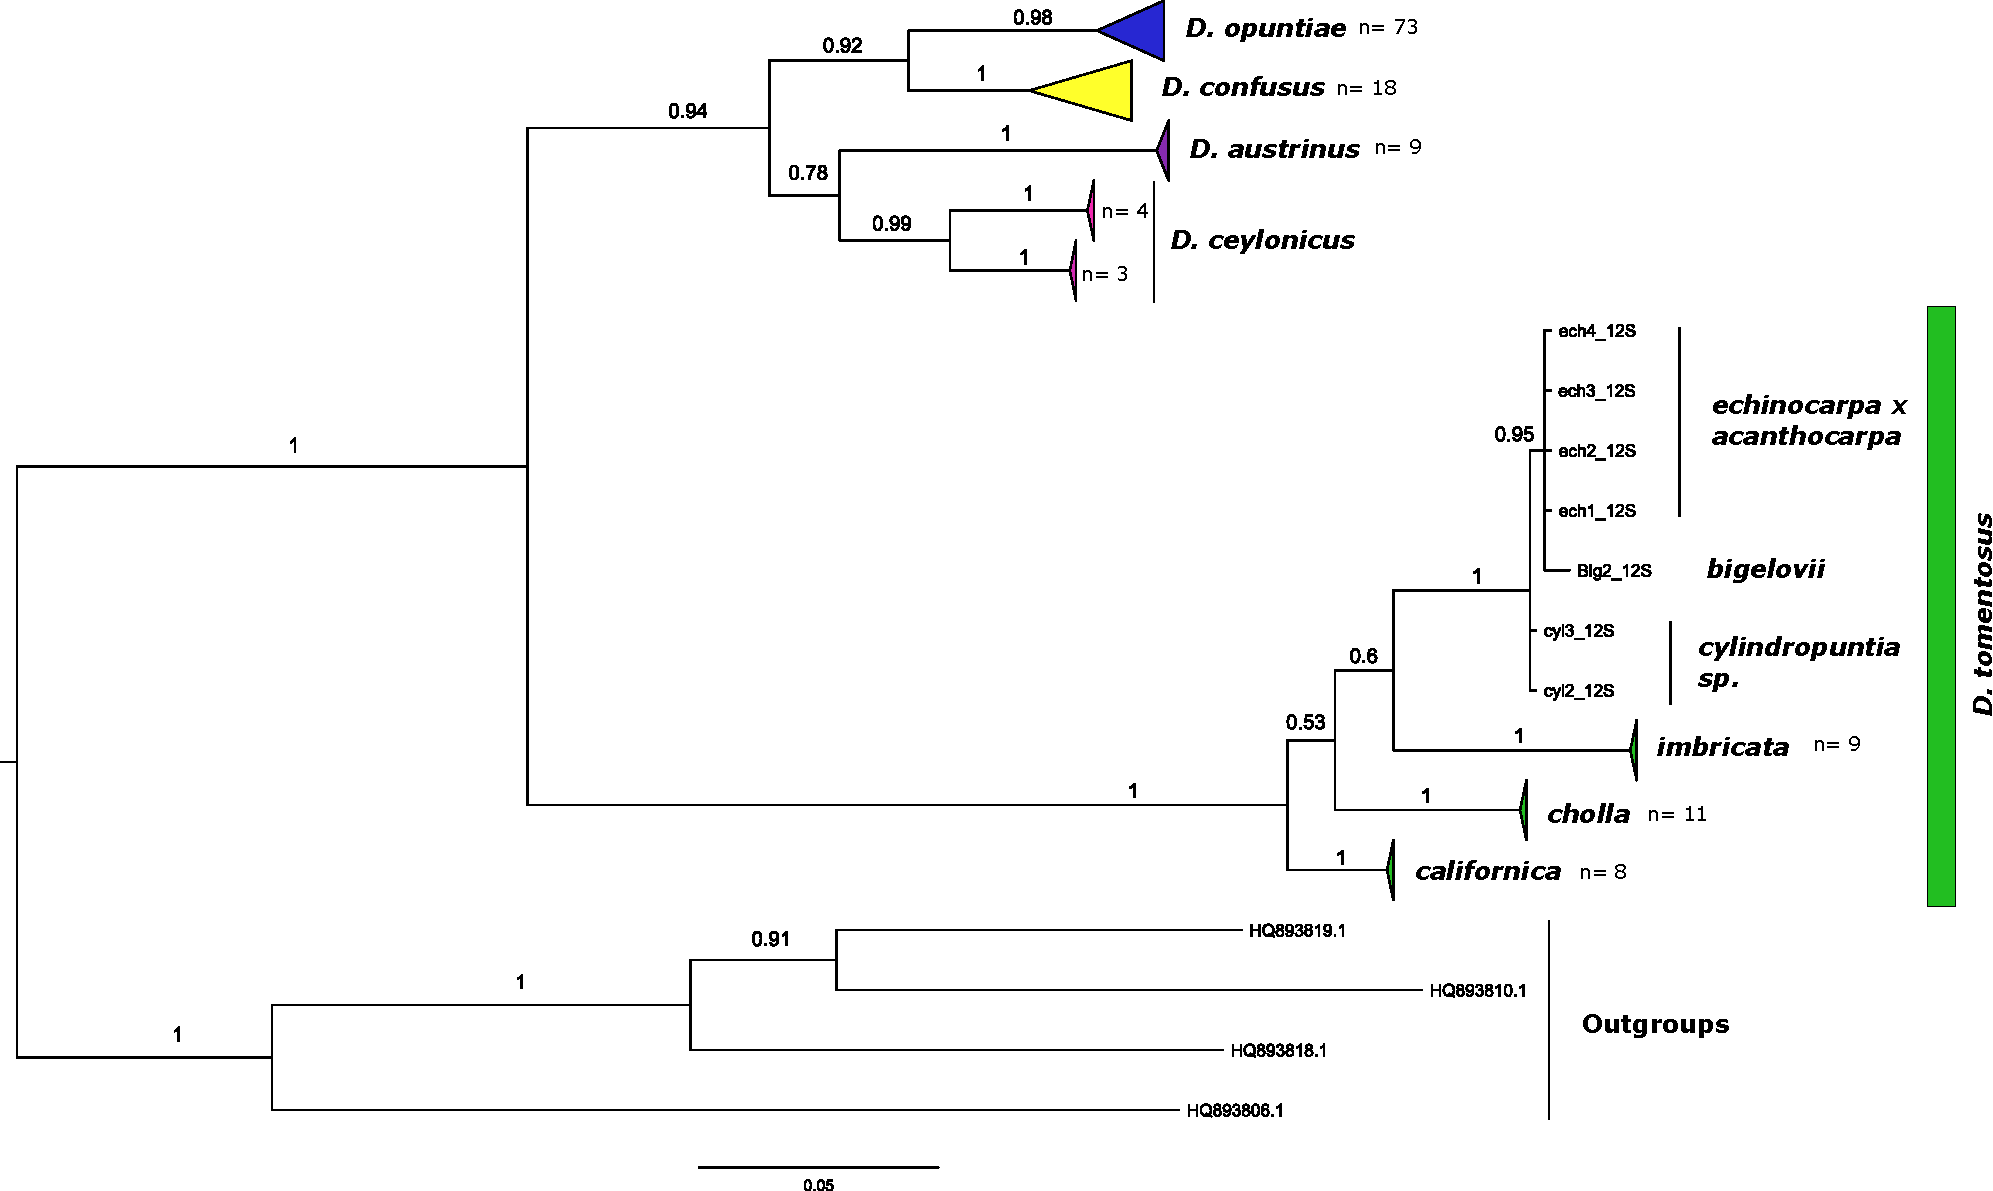
\includegraphics[scale =0.7]{Images/12S_rcoffee_collapsed_export.pdf}
	\caption{12S rRNA Bayesian phylogeny based on the alignment obtained from R-Coffee, which aligns RNA sequences according to their secondary structure. The HKY + I + G model was used, where shapepr = 0.9980, pinvarp = 0.1420 and tratiopr = 1.4096. State frequencies were 0.5155, 0.0897, 0.0282 and 0.3665. Major clades have been collapsed.}  
	\label{fig:12S_rcoffee}
\end{figure}

\end{landscape}

\section{Program settings and file formats}
\subsection{GeneMarker}
\label{appendix:genemarker_settings}

\begin{enumerate}
    \item Size standard set to `GS500LIZ' (Size editor $\rightarrow$ File $\rightarrow$ Import ABI Size Standard $\rightarrow$ select the desired size standard file) and Analysis Type to `AFLP'.
    \item The selected Raw Data Analysis settings were: Auto Range (frame), Saturation Repair, Baseline Subtraction, Pull-up Correction, Spike Removal and Local Southern.
    \item Allele Call settings were: Allele calls set to the `automatic'. Minimum Intensity for peak detection set at 50 RFU (relative fluorescence units) and Max Intensity left at the default (30000 RFU). This minimum intensity is recommended by \citet{arrigo2012automated} as a more permissive prior screening approach. \citet{prince2009} used an even lower threshold, set at 20 RFU. Peaks below the threshold are most likely due to the slippage of polymerase during the PCR elongation step, sometimes referred to as `taq stutter' \citep{DNAFragAnalysis, prince2009}. Plus-A Filter was left selected.
    \item `AFLP normalization' selected.
    \item The summary table was obtained by selecting `Report settings' followed by `Peak Table'. The `Abide by Panel', `Show Only Uncertain Alleles' and `Show Rejected Low Score Alleles' options were deselected, and the * symbol in the `Show * when no allele call is unchecked' option was deleted and left blank. Peak reads were subsequently converted into a summary table that was exported as a .txt file.
\end{enumerate}

\subsection{POPART}
\label{appendix:popart}
POPART reads in files in Nexus format, following the minimal working example below. In the `begin traits' section, the trait label index number corresponds to the column number for each sequence (i.e. a `1' in the first column = Africa, in the second column = the USA and the third column = Asia), such that sequenceA and sequenceC represents Africa, sequenceB the USA and sequenceD Asia. \\

\noindent \# NEXUS \\
begin data; \\
dimensions ntax=4 nchar=4; \\
format datatype=dna missing=N gap = -; \\
\noindent matrix \\
\noindent sequenceA \hspace{0.5cm} ACTG \\
sequenceB \hspace{0.5cm} ACGG \\
sequenceC \hspace{0.5cm}  ACTT \\
sequenceD \hspace{0.5cm}  ACCC \\
; \\
end; \\
\noindent begin traits; \\
Dimensions ntraits=3; \\
Format labels=yes separator=Comma; \\
TraitLabels Africa, USA, Asia; \\
matrix \\ 
\noindent sequenceA \hspace{0.5cm} 1,0,0 \\
sequenceB \hspace{0.5cm} 0,1,0 \\
sequenceC \hspace{0.5cm} 1,0,0 \\
sequenceD \hspace{0.5cm} 0,0,1 \\
; \\
end; \\

\subsection{SplitsTree}
\label{appendix:splitstree_input}

\noindent{\#NEXUS} \\
BEGIN Taxa; \\
DIMENSIONS NTAX = 2; \\
END; \\
BEGIN Characters; \\
DIMENSIONS NCHAR = 4; \\
FORMAT DATATYPE = STANDARD INTERLEAVE MISSING = ?; \\
MATRIX \\
Seq1 001? \\
Seq2 11?? \\ 
; \\ 
END;  

\subsection{STRUCTURE}
\label{appendix:structure_settings}

Binary data were organised in Microsoft Excel\textsuperscript{\textregistered} according to the example format below. Question mark (`?') symbols replaced with `-9', saved as a tab-delimited .txt file, and uploaded to STRUCTURE. Column 2 contained integers specifying population groupings, referred to as `PopData' in the STRUCTURE user manual. These groupings are not used as priors by default, and are otherwise useful to organise the graphical output produced by CLUMPAK \citep{Kopelman2015} (available at \url{http://clumpak.tau.ac.il/index.html}). \\

\begin{table}[H]
\centering
\begin{tabular}{@{}llccc@{}}
 &  & Locus 1 & Locus 2 & Locus 3 \\
Sample1 & 1 & 0 & 1 & -9 \\
Sample2 & 1 & 0 & 1 & 1 \\
Sample3 & 2 & 1 & 1 & 1 \\
Sample4 & 2 & -9 & 0 & 0
\end{tabular}
\end{table}

Ploidy was set to 1, missing data to -9, `Row of marker names' and `individual ID for each individual' were selected, as well as `Putative population origin for each individual'. \textit{K} was set from 1 through to at least four times the expected number of lineages to ensure thorough sampling. 20 iterations were run for each value of \textit{K} to ensure reliable output, with a burn-in of 100 000, followed by 50 000 MCMC runs (following the recommendations made by \citet{wang2017computer} and \citet{puechmaille2016program}). \citet{puechmaille2016program} found that increasing the burn-in and/or MCMC runs above these values had no further effect on the result. The `Population admixture model' and `Allele frequencies correlated' were selected (recommended by \citet{falush2003inference} and tested by \citet{puechmaille2016program}). All other parameters were left at their default settings (similar to the approach made by \citet{Sutton2017GeneticAgents}, and \citet{medrano2014population}).

\section{Jaccard's transformation}
\label{appendix:jaccards_transformation}

\vspace{0.5cm}
\begin{figure}[H]
	\centering
	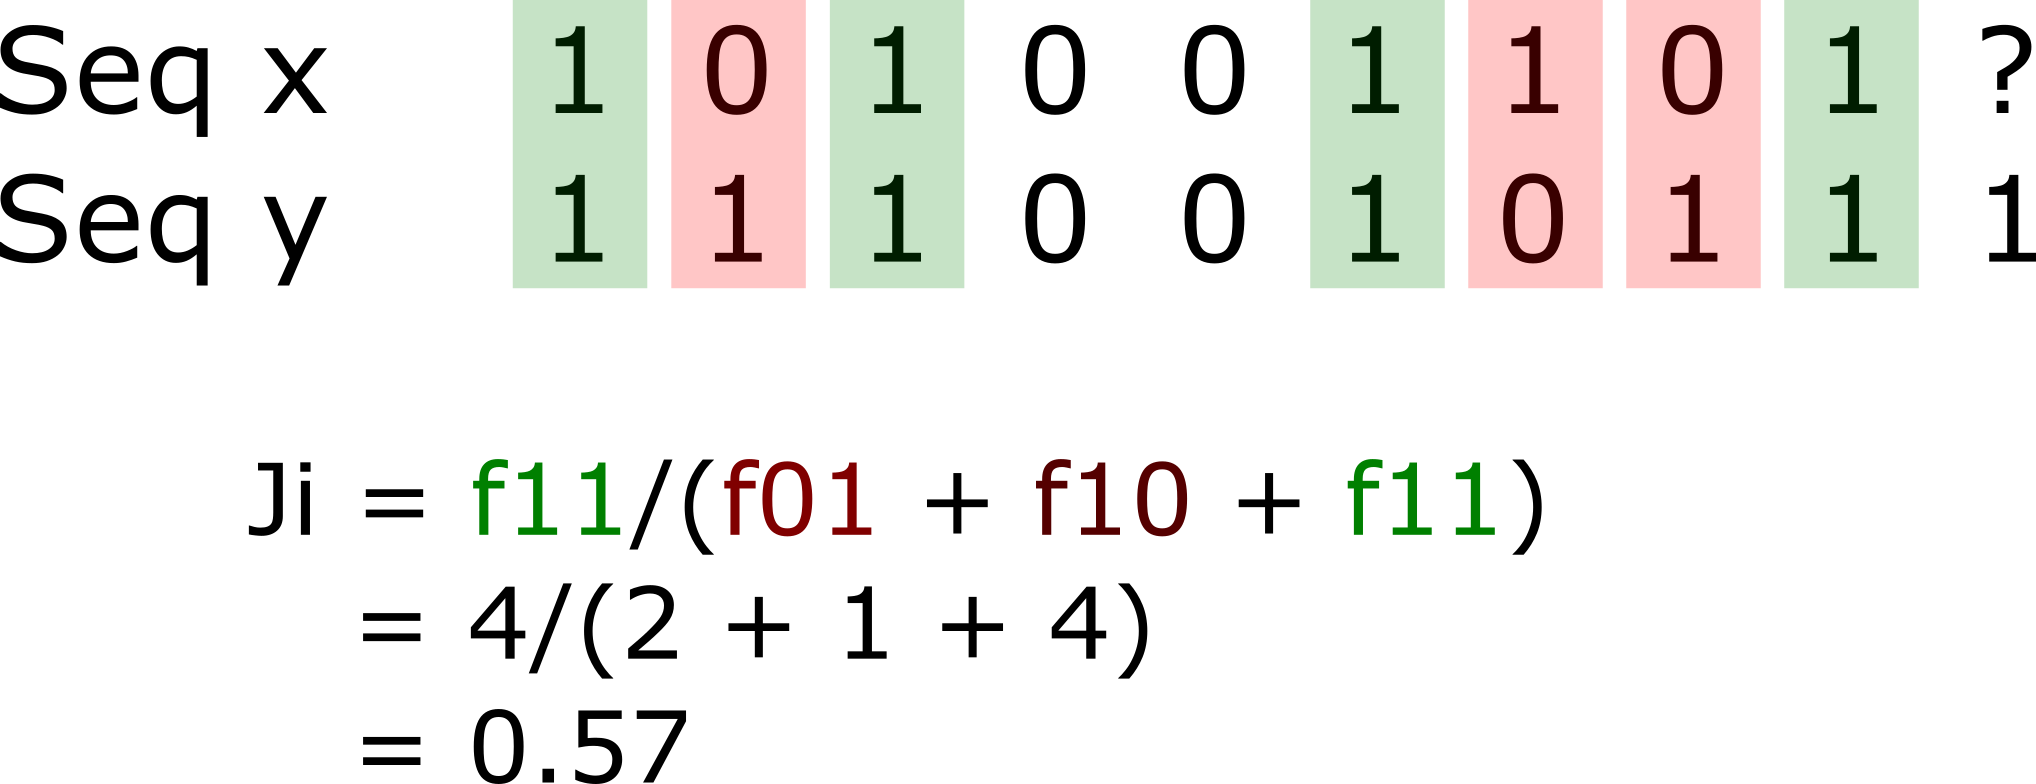
\includegraphics[scale = 1.3]{Images/jaccard}
    \newline
	\caption{An example of Jaccard's similarity index calculation. Note that the shared absence of bands are not taken into account in the calculation of pairwise distances. Jaccard's distance = 1 - J\textsubscript{i}, and therefore 0.43 in this case.}. 
	\label{fig:jaccard}
\end{figure}

% \section{Codon Saturation}

% \label{appendix:saturation}
% \begin{figure}[H]
% 	\centering
% 	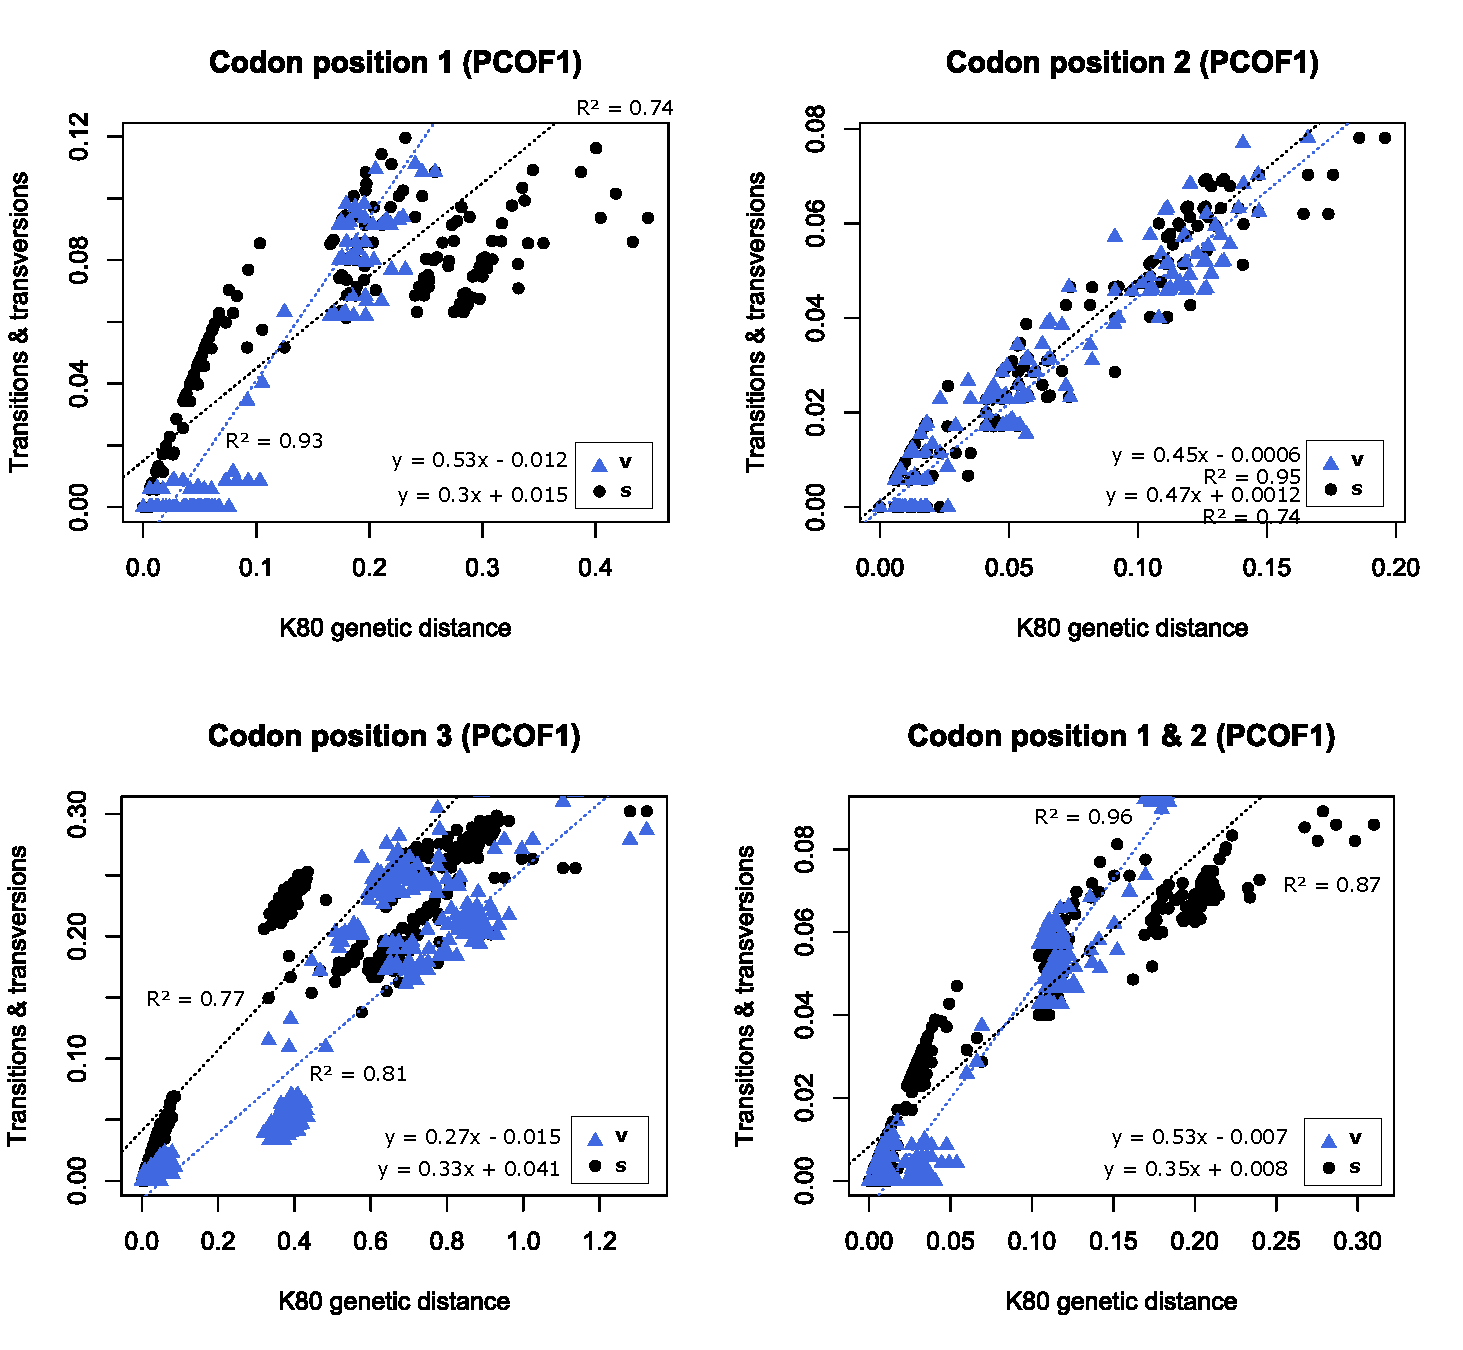
\includegraphics[scale =0.7]{Images/PCOF1_saturation.pdf}
% 	\caption{Transitions (s) and transversions (v) plotted against the K80 genetic distance for the PCOF1 gene at codon positions 1, 2, 3 and 1 \& 2. Equations of the best fit lines are shown, as well as the R\textsuperscript{2} value.}  
% 	\label{fig:pcof1_saturation}
% \end{figure}

% \begin{figure}[H]
% 	\centering
% 	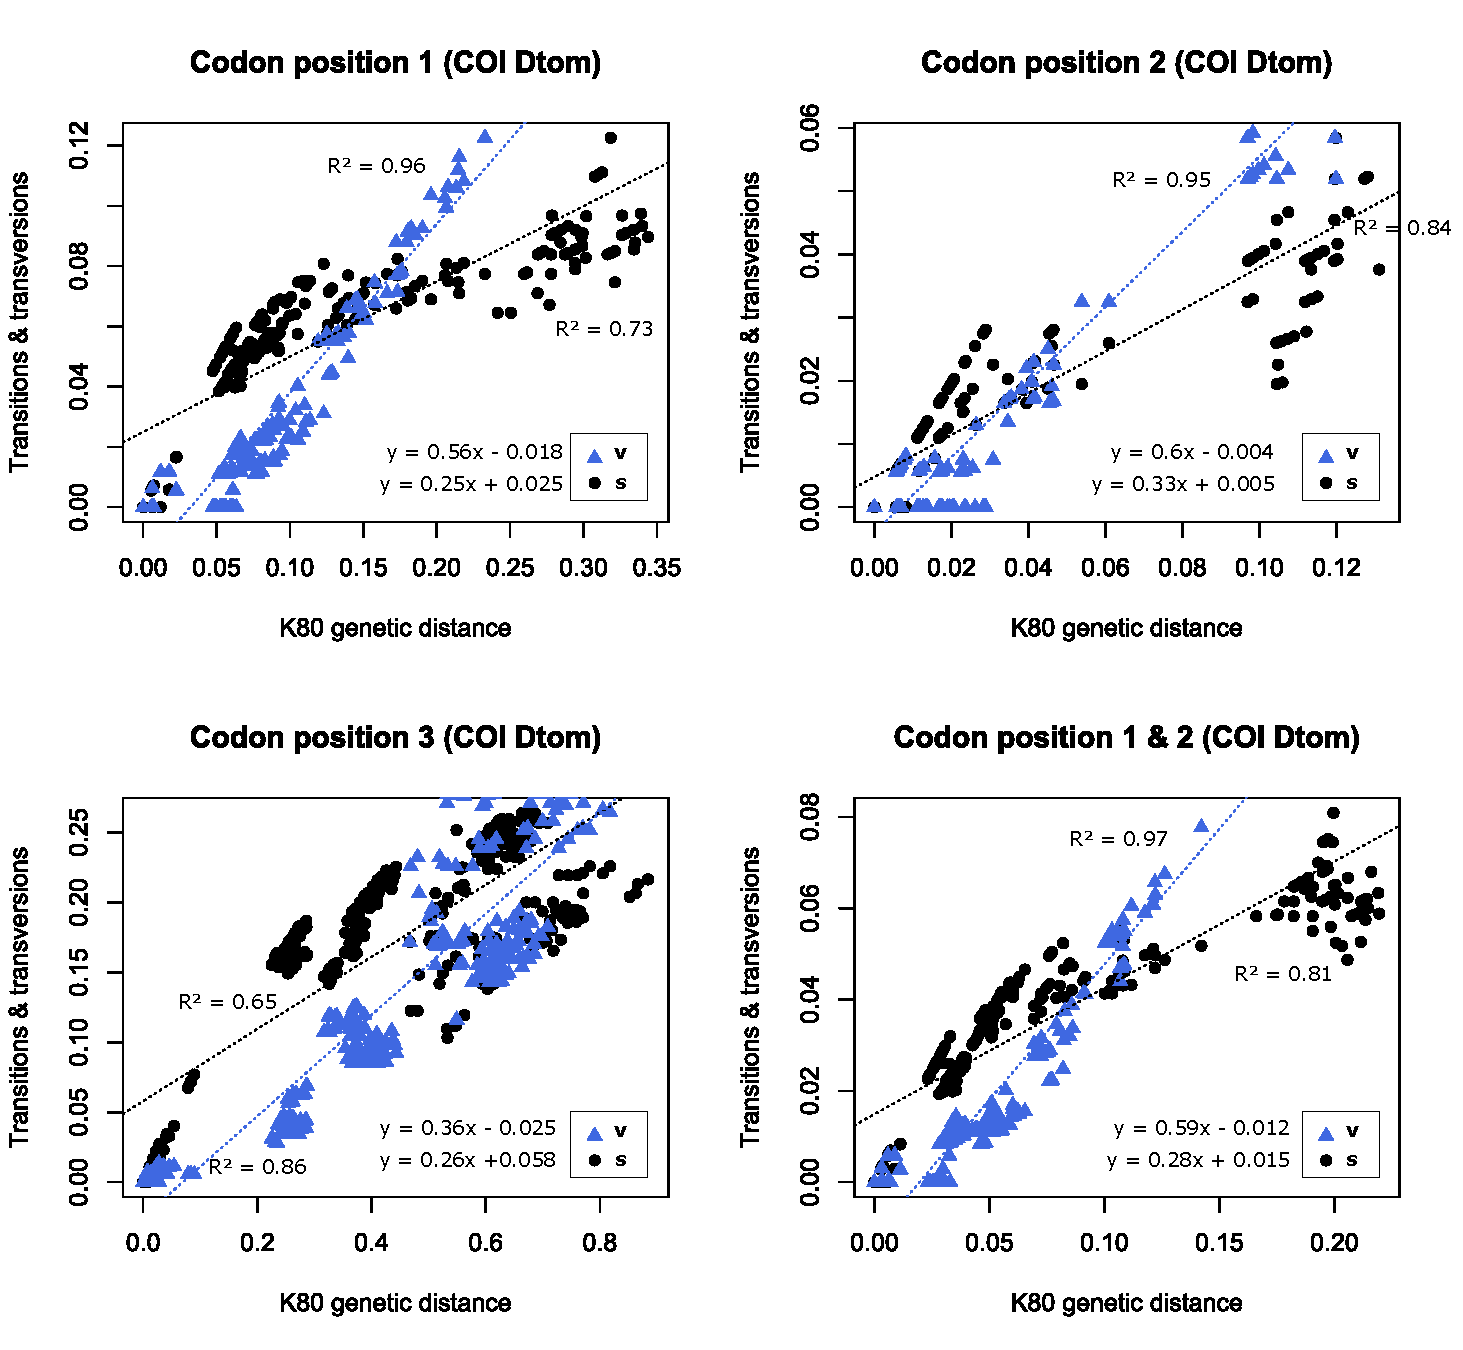
\includegraphics[scale =0.7]{Images/COIDtom_saturation.pdf}
% 	\caption{Transitions (s) and transversions (v) plotted against the K80 genetic distance for the COI (Dtom) gene at codon positions 1, 2, 3 and 1 \& 2. Equations of the best fit lines are shown, as well as the R\textsuperscript{2} value.} 
% 	\label{fig:co1_dtom_saturation}
% \end{figure}

\section{Codon saturation}

\vspace{0.5cm}
\begin{table}[H]
\renewcommand{\arraystretch}{0.4}
\caption{Codon saturation results from DAMBE for the protein-coding COI-A and COI-B gene regions. A significant p-value and an Iss value $<$ the Iss.cSym value means that there is little saturation present.}
\label{tab:saturation}
\centering
\begin{tabular}{@{}lllllll@{}}
\toprule
 & \textbf{NumOTU} & \textbf{Iss} & \textbf{Iss.cSym} & \textbf{T} & \textbf{DF} & \textbf{P} \\ \midrule
\textbf{\begin{tabular}[c]{@{}l@{}}Codon\\ Position 1\end{tabular}} & \textbf{4} & 0.357 & 0.777 & 10.403 & 200 & 0 \\
 & \textbf{8} & 0.327 & 0.734 & 10.155 & 200 & 0 \\
 & \textbf{16} & 0.311 & 0.643 & 8.428 & 200 & 0 \\
\textbf{\begin{tabular}[c]{@{}l@{}}Codon\\ Position 2\end{tabular}} & \textbf{4} & 0.273 & 0.777 & 12.203 & 200 & 0 \\
 & \textbf{8} & 0.227 & 0.734 & 12.727 & 200 & 0 \\
 & \textbf{16} & 0.228 & 0.643 & 10.415 & 200 & 0 \\
\textbf{\begin{tabular}[c]{@{}l@{}}Codon\\ Position 3\end{tabular}} & \textbf{4} & 0.578 & 0.777 & 4.956 & 200 & 0 \\
 & \textbf{8} & 0.539 & 0.734 & 4.979 & 200 & 0 \\
 & \textbf{16} & 0.534 & 0.643 & 2.843 & 200 & 0 \\
\textbf{\begin{tabular}[c]{@{}l@{}}Codon\\ Position 1 \& 2\end{tabular}} & \textbf{4} & 0.334 & 0.788 & 14.989 & 401 & 0 \\
 & \textbf{8} & 0.274 & 0.742 & 16.002 & 401 & 0 \\
 & \textbf{16} & 0.260 & 0.702 & 15.465 & 401 & 0 \\ \bottomrule
\end{tabular}
\end{table}

\begin{landscape}
\begin{figure}[]
	\centering
	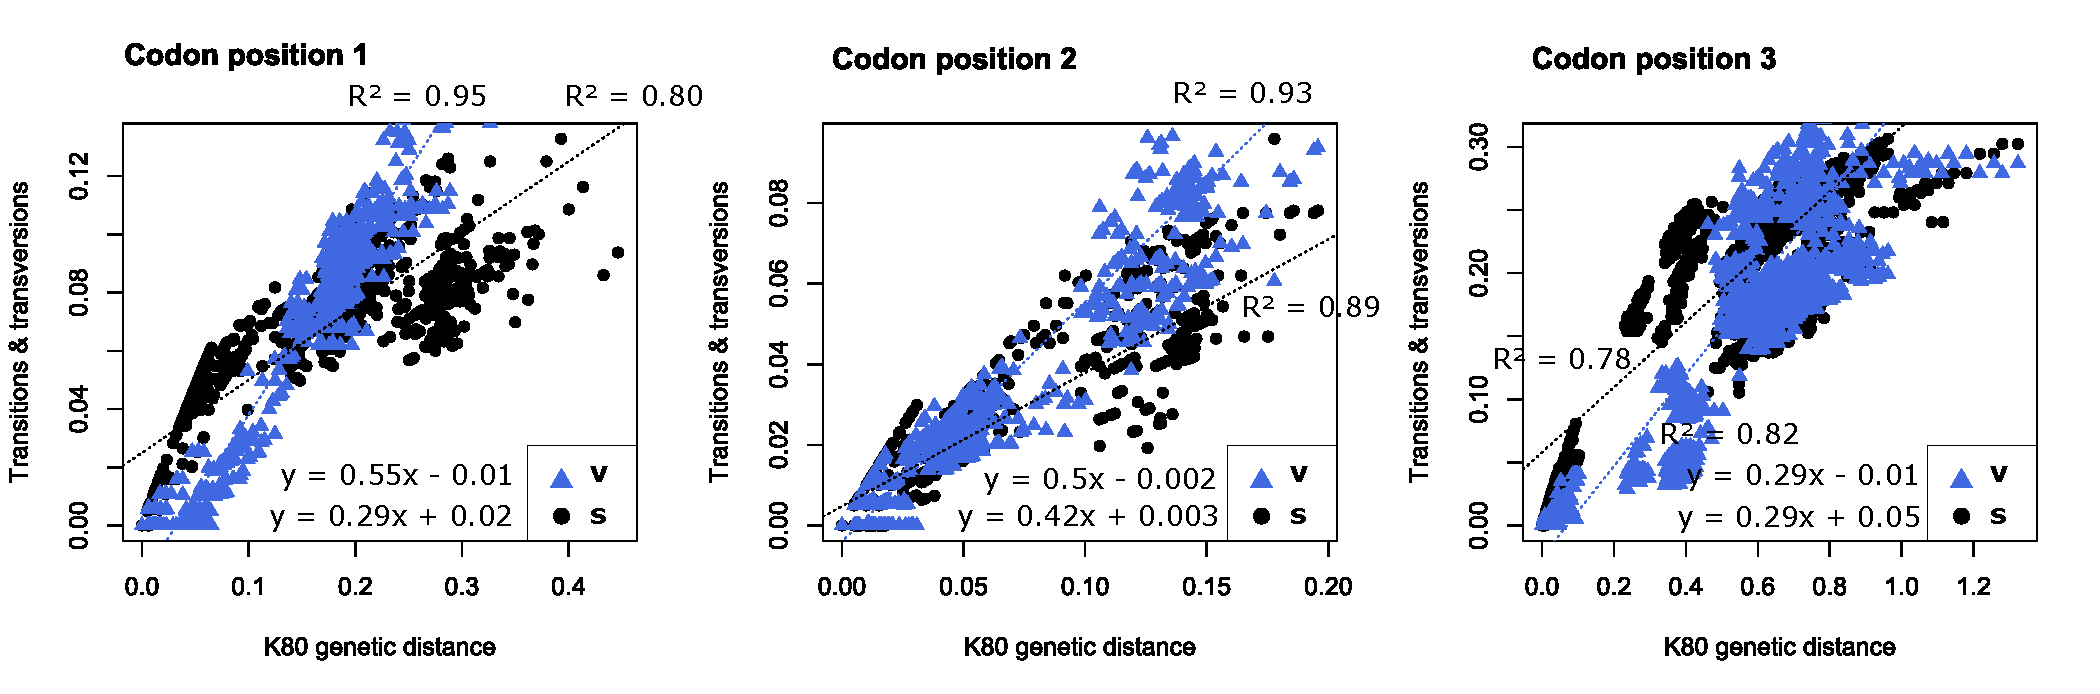
\includegraphics[scale =0.75]{Images/saturation_COI.pdf}
	\caption{Saturation graphs for codon positions 1 to 3 for the COI gene region; showing the relationship between genetic distance and the rate of transitions (s) and transversions (v).}
	\label{fig:COI_saturation_graphs}
\end{figure}
\end{landscape}


% \section{Barcode testing thresholds}

% \begin{figure}[H]
% 	\centering
% 	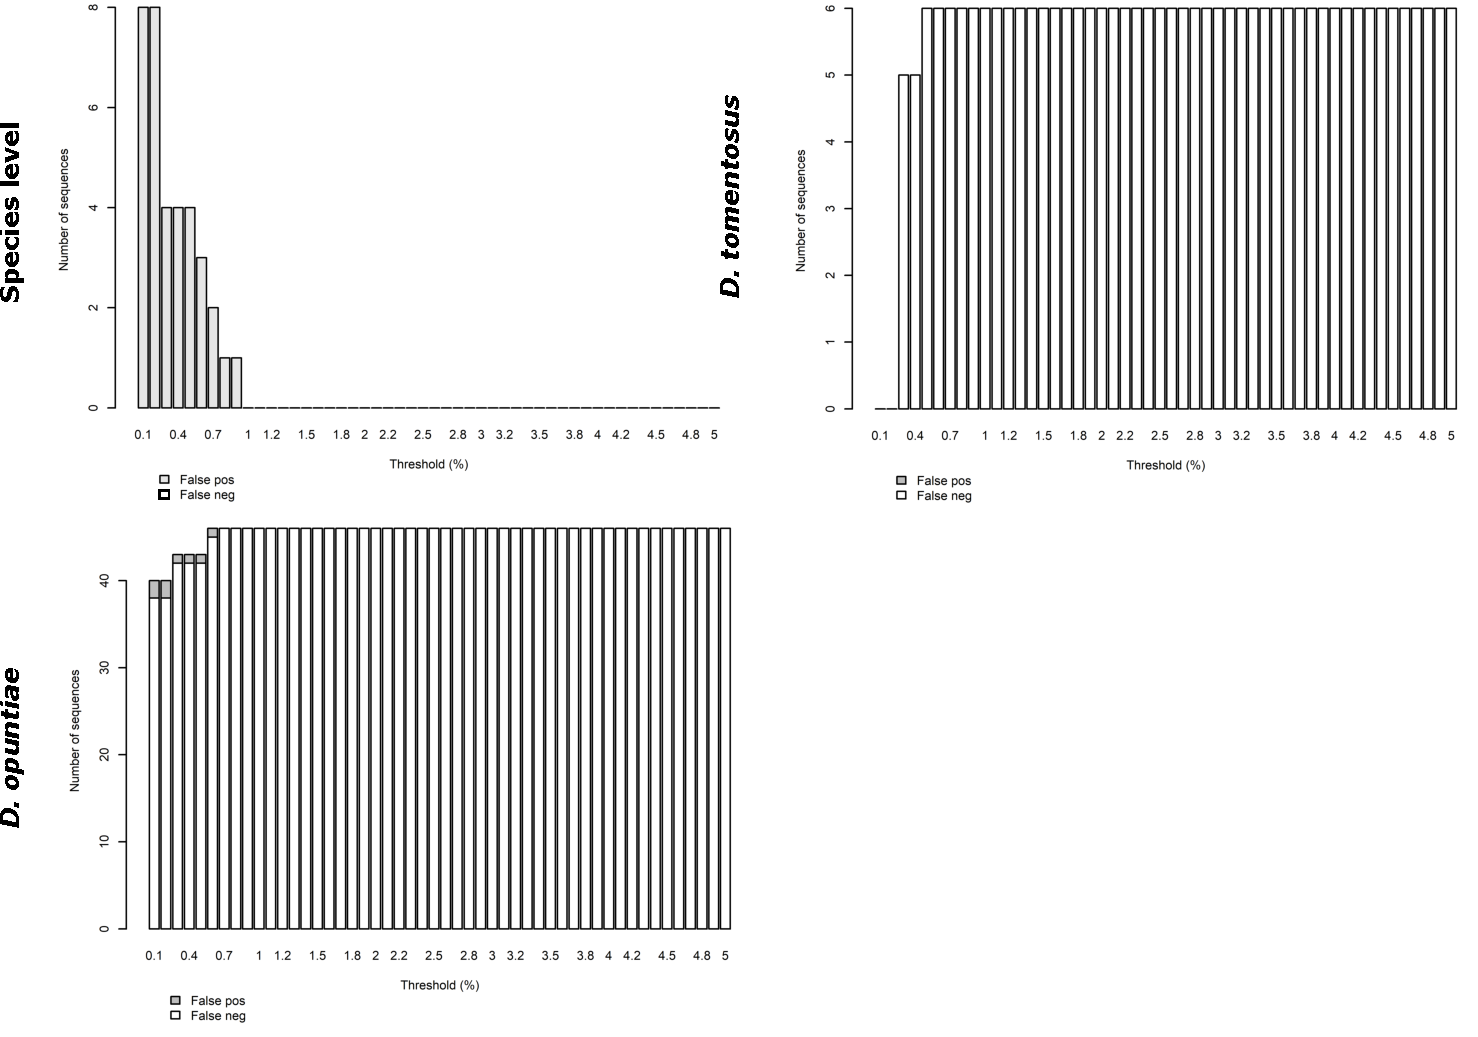
\includegraphics[scale =0.7]{Images/12S_thresholds.pdf}
% 	\caption{Genetic distance threshold values for the 12S gene at the species and lineage level. The optimal threshold percentage at the species level is at 1\% and 0.2\% for \textit{D. tomentosus} lineages. \textit{Dactylopius opuntiae} lineages did not have an optimal threshold value, with a high number of false negatives.} 
% 	\label{fig:12S_thresh}
% \end{figure}

% \begin{figure}[H]
% 	\centering
% 	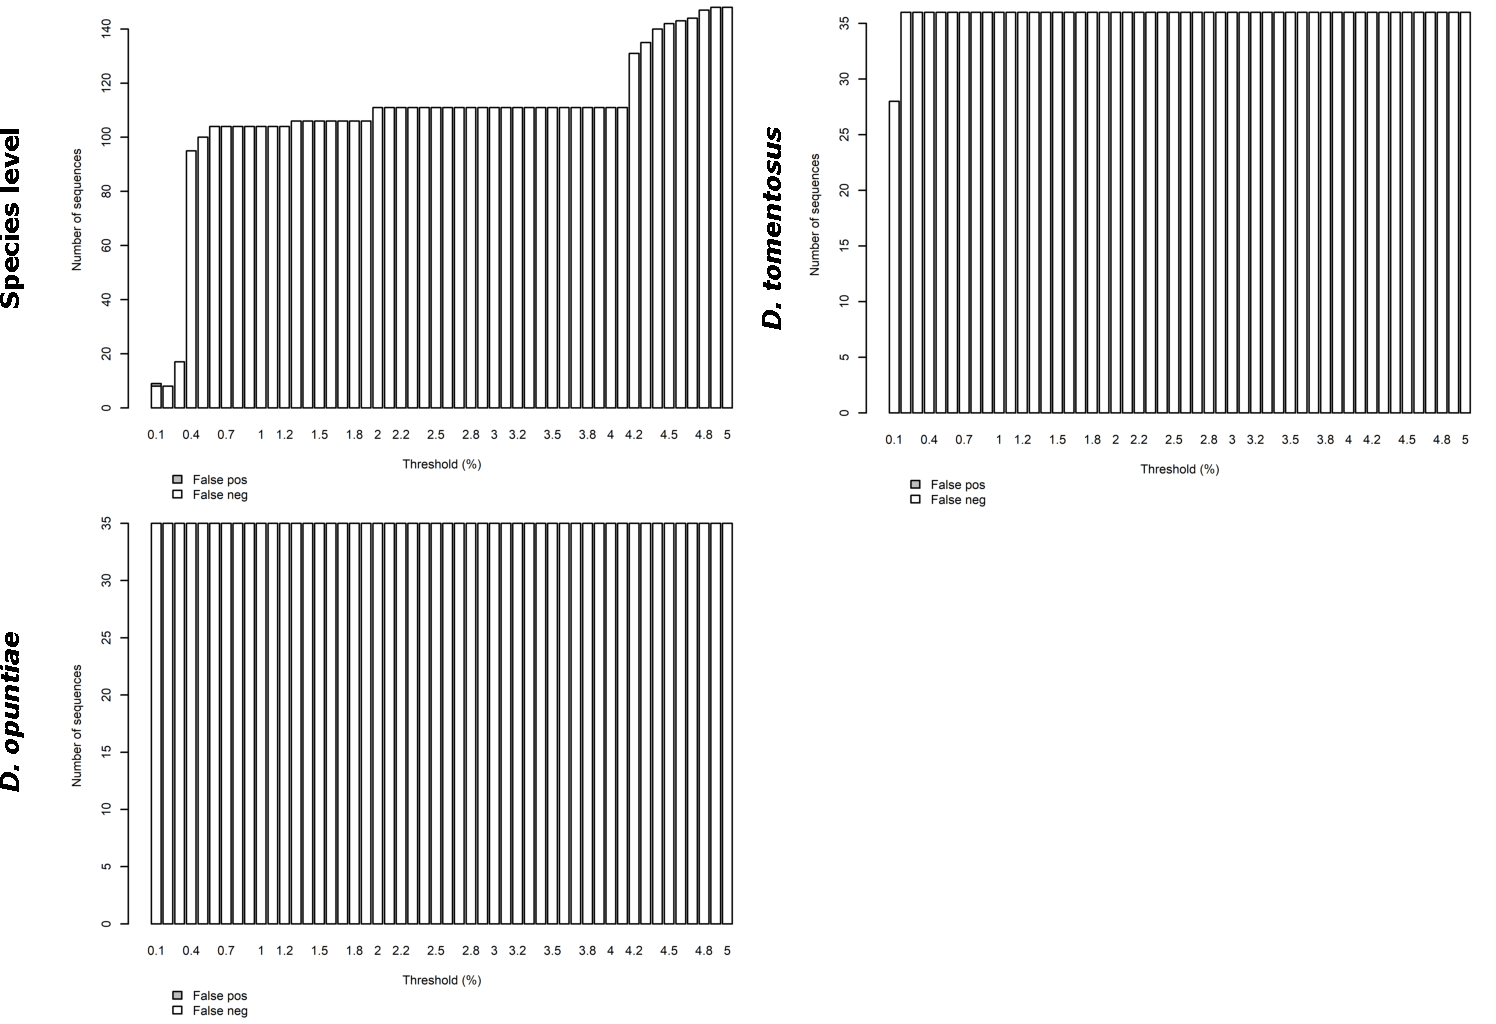
\includegraphics[scale =0.7]{Images/thresholds_18S.pdf}
% 	\caption{Genetic distance threshold values for the 18S gene at the species and lineage level. The optimal threshold value at the species level is 0.2\%. At the lineage level, both \textit{D. tomentosus} and \textit{D. opuntiae} showed a high level of false negatives.} 
% 	\label{fig:18SThresh}
% \end{figure}

% \begin{figure}[H]
% 	\centering
% 	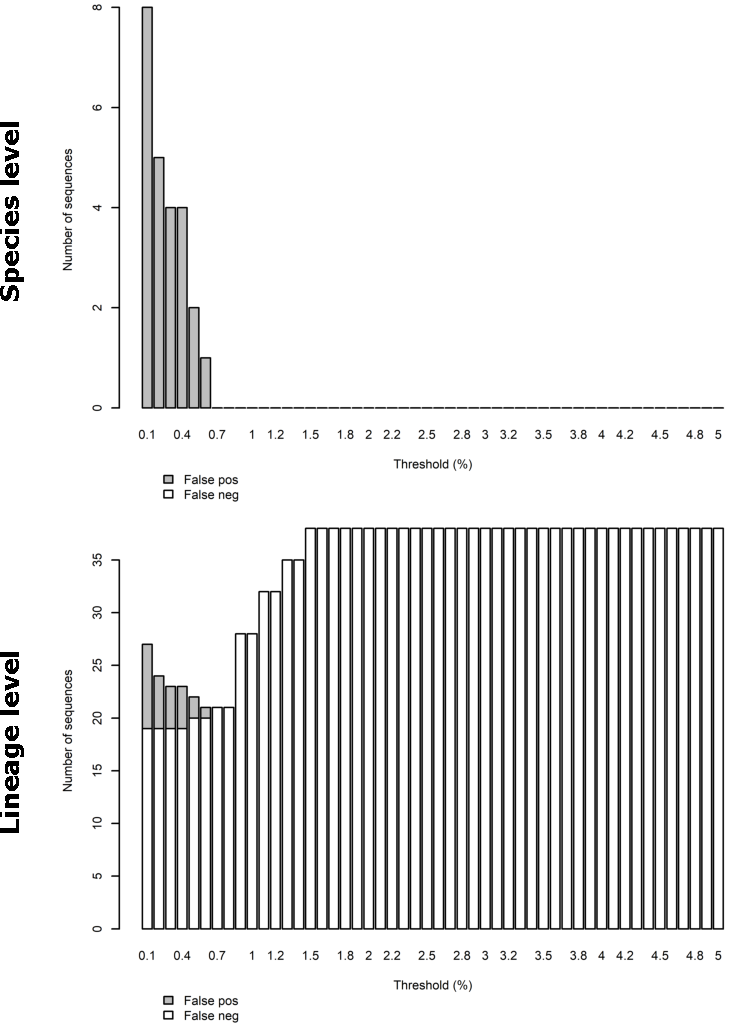
\includegraphics[scale =1]{Images/PCOF1_thresholds.pdf}
% 	\caption{Genetic distance threshold values for the PCOF1 \& LepR1 at the lineage and species level. The optimal threshold value at the species level is 0.7\%. The lineage level (\textit{D. opuntiae}) showed a high number of false negatives.} 
% 	\label{fig:pcof1Thresholds}
% \end{figure}

% \begin{figure}[H]
% 	\centering
% 	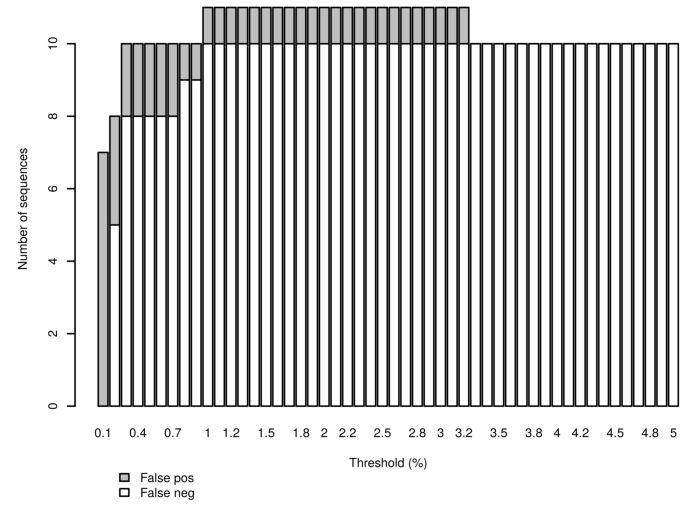
\includegraphics[scale =0.8]{Images/thresholdGraph_DTOM2.pdf}
% 	\caption{Genetic distance threshold values for DTOMf \& HCO2198 at the \textit{D. tomentosus} lineage level. `Bigelovii' and `echinocarpa x acanthocarpa' are treated as separate lineages.} 
% 	\label{fig:COIDTOM_thresh}
% \end{figure}

% \begin{figure}[H]
% 	\centering
% 	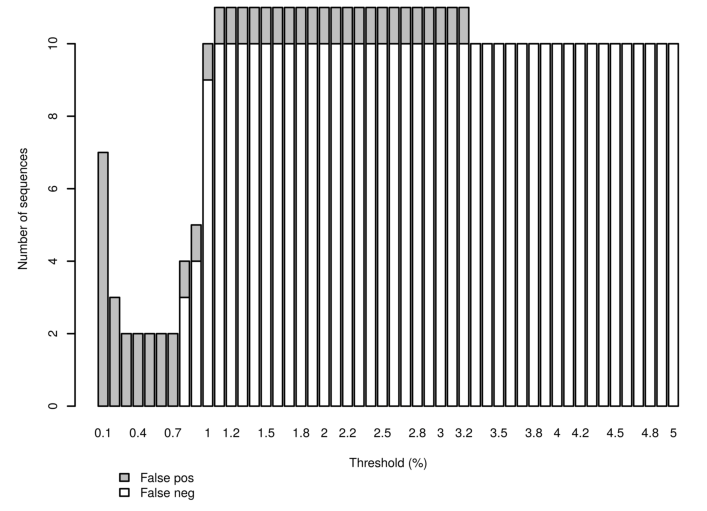
\includegraphics[scale =0.8]{Images/thresholdGraph2.pdf}
% 	\caption{Genetic distance threshold values for DTOMf \& HCO2198 at the \textit{D. tomentosus} lineage level. `Bigelovii' and `echinocarpa x acanthocarpa' are grouped as one lineage.} 
% 	\label{fig:COIDTOM_thresh2}
% \end{figure}

% \begin{figure}[H]
% 	\centering
% 	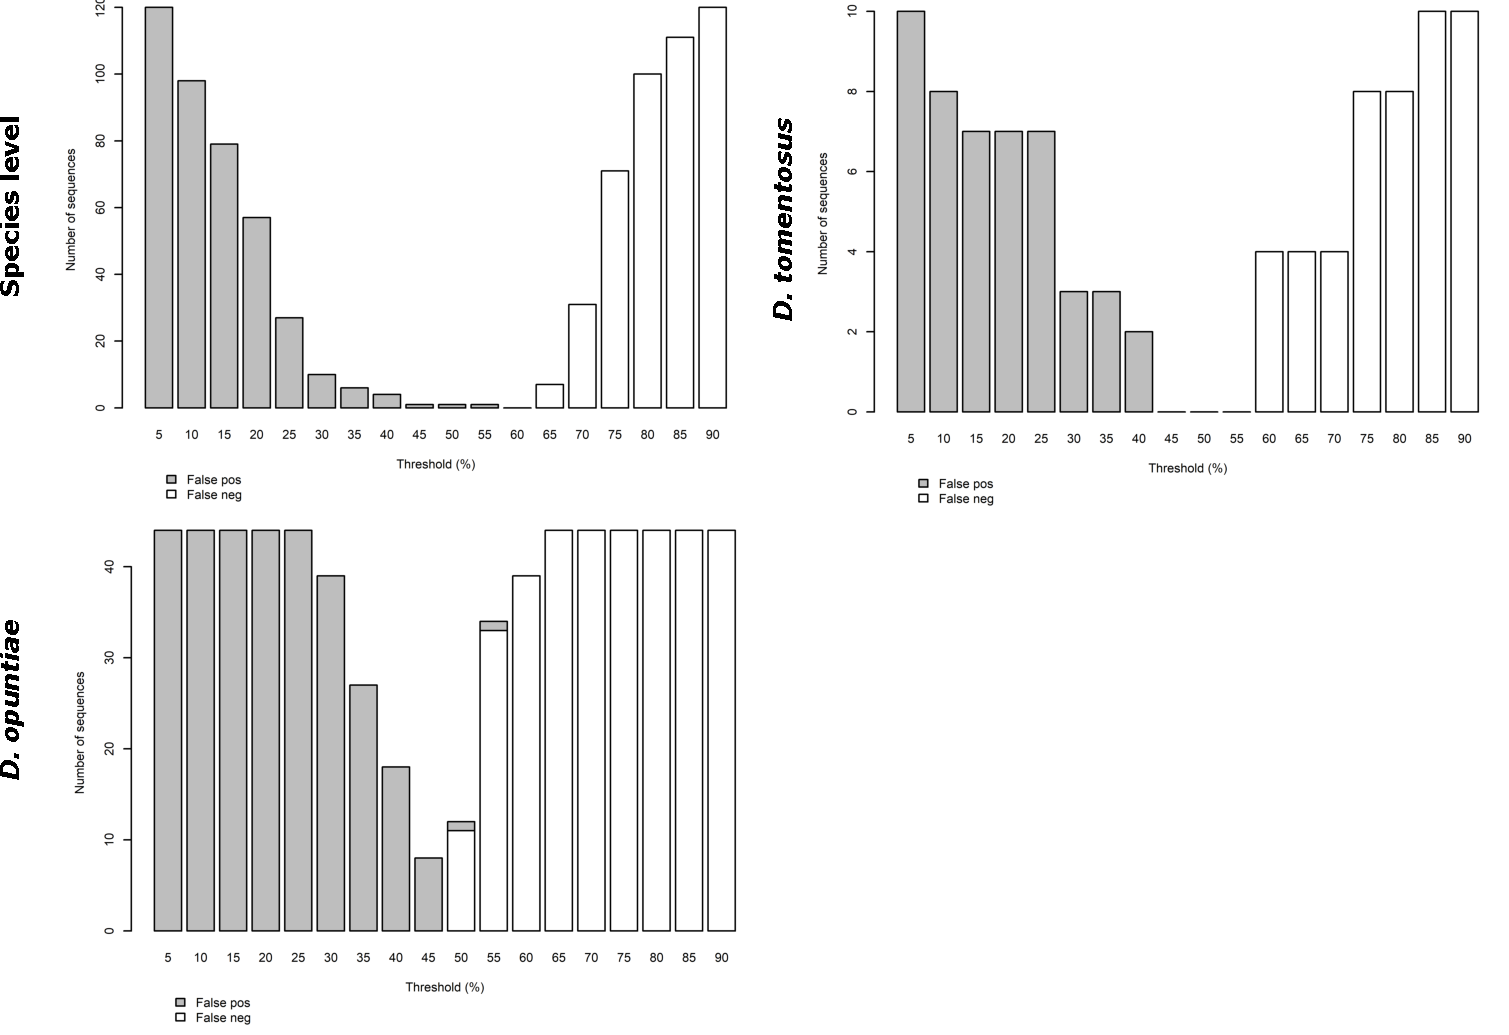
\includegraphics[scale =0.67]{Images/thresholds_issrs.pdf}
% 	\caption{Genetic distance threshold values for the species level, \textit{D. opuntiae} and \textit{D. tomentosus} lineages, for all \textit{Dactylopius} samples.} 
% 	\label{fig:ISSR_thresh}
% \end{figure}

% \section{Barcode Gaps}

% \begin{figure}[H]
% 	\centering
% 	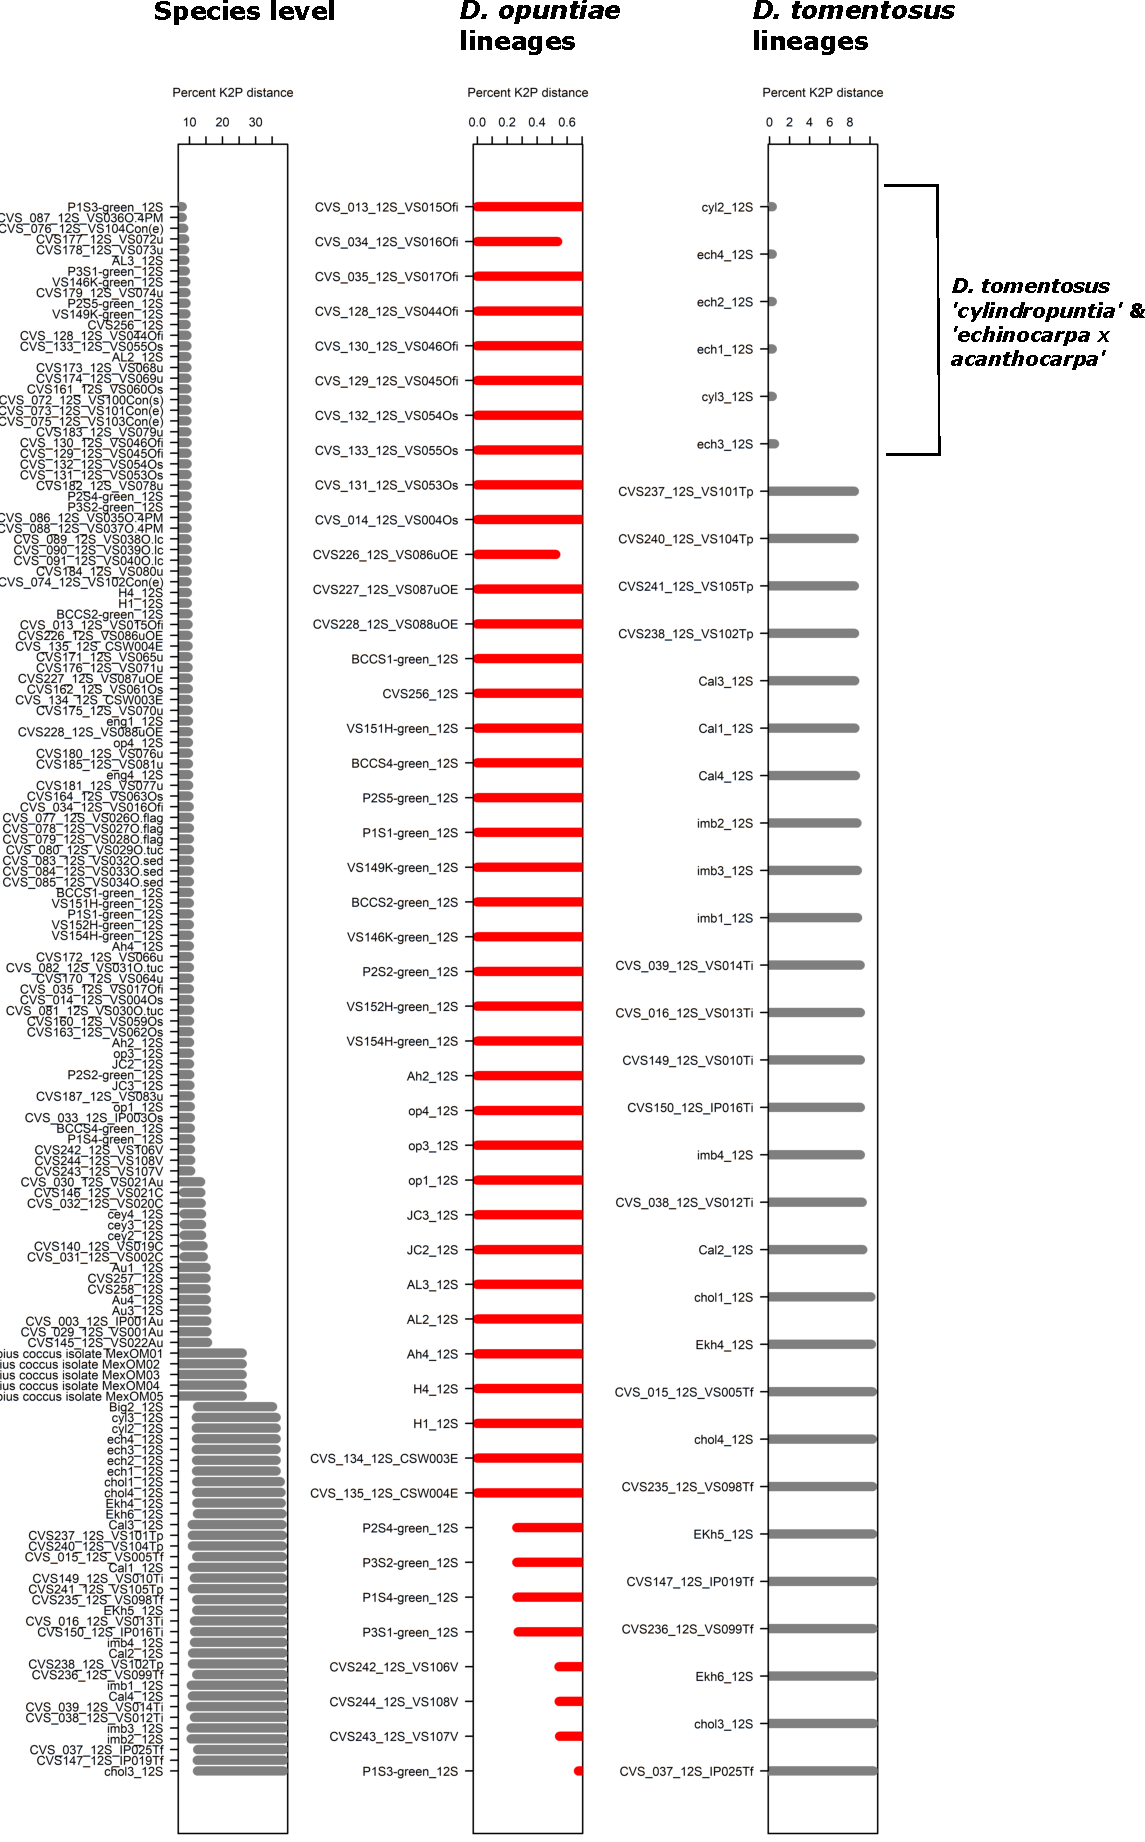
\includegraphics[scale =0.65]{Images/12S_barcode_gaps.pdf}
% 	\caption{Barcode gaps for the 12S gene at the lineage  and species levels. Red bars indicate instances where the intraspecific distance $>$ than the interspecific distance for a particular sequence (i.e. a negative barcode gap). The presence of positive barcode gaps underlies the success of genetic barcoding.} 
% 	\label{fig:12SBarcodeGap}
% \end{figure}

% \begin{figure}[H]
% 	\centering
% 	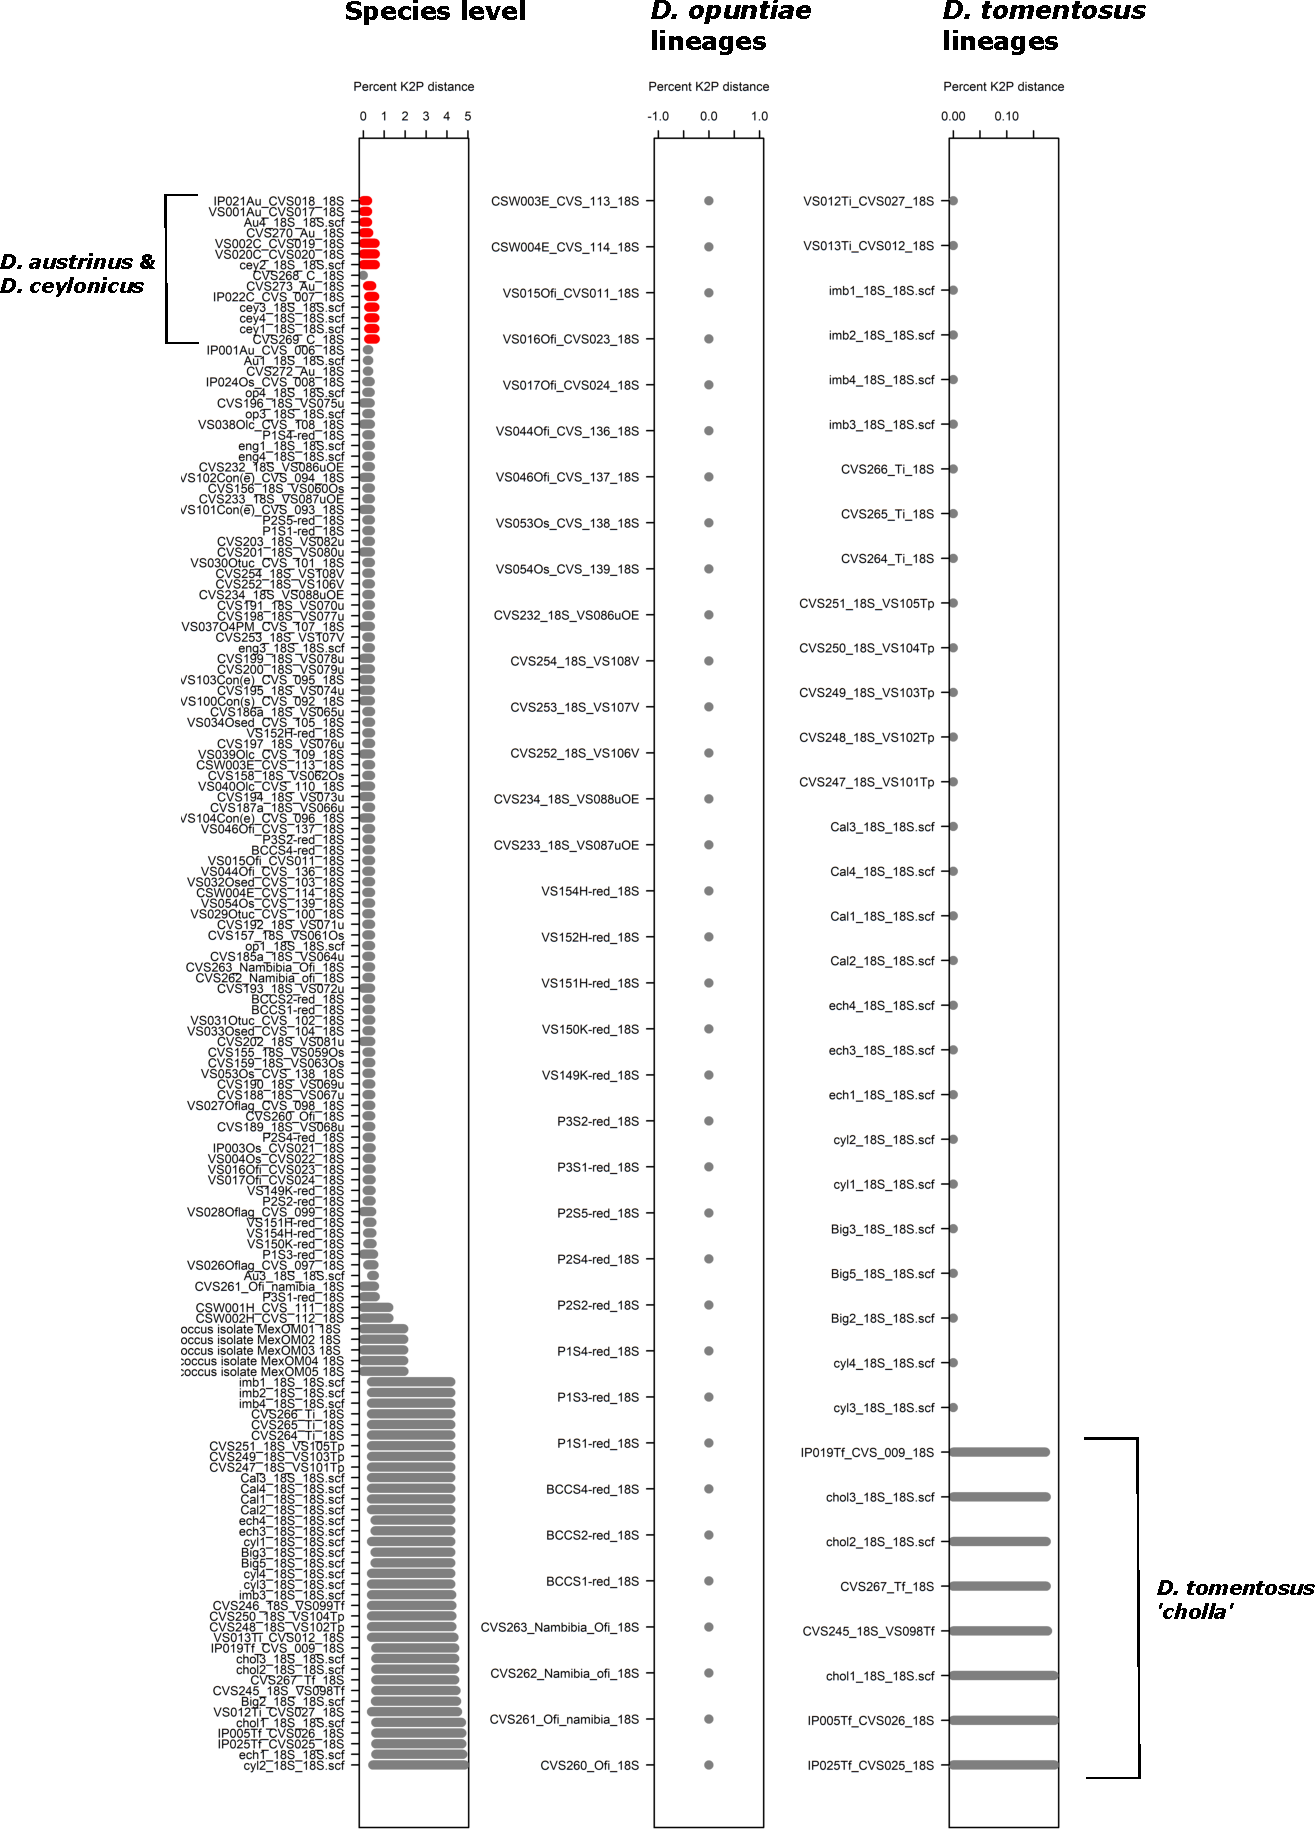
\includegraphics[scale =0.7]{Images/barcode_gaps_18S.pdf}
% 	\caption{Barcode gaps for the 18S gene at the lineage and species level. Note the smaller scale on the lineage-level graphs.} 
% 	\label{fig:18SBarcodeGap}
% \end{figure}

% \begin{figure}[H]
% 	\centering
% 	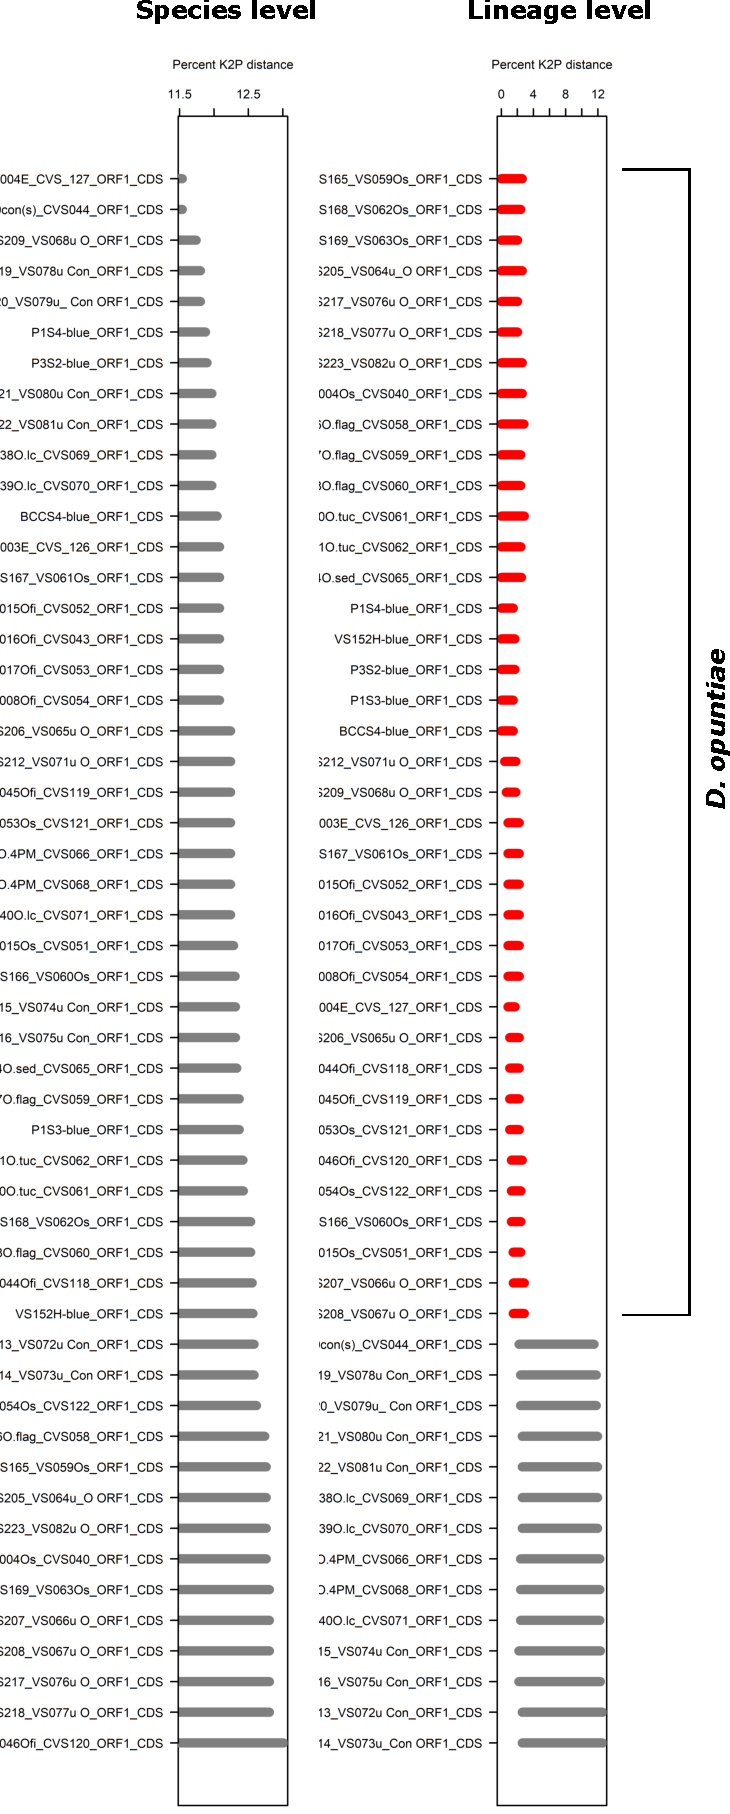
\includegraphics[scale =0.75]{Images/PCOF1_barcode_gaps.pdf}
% 	\caption{Barcode gaps for PCOF1 \& LepR1 at the species and lineage level.} 
% 	\label{fig:COI_barcodeGap}
% \end{figure}

% \newpage

% \begin{figure}[H]
% 	\centering
% 	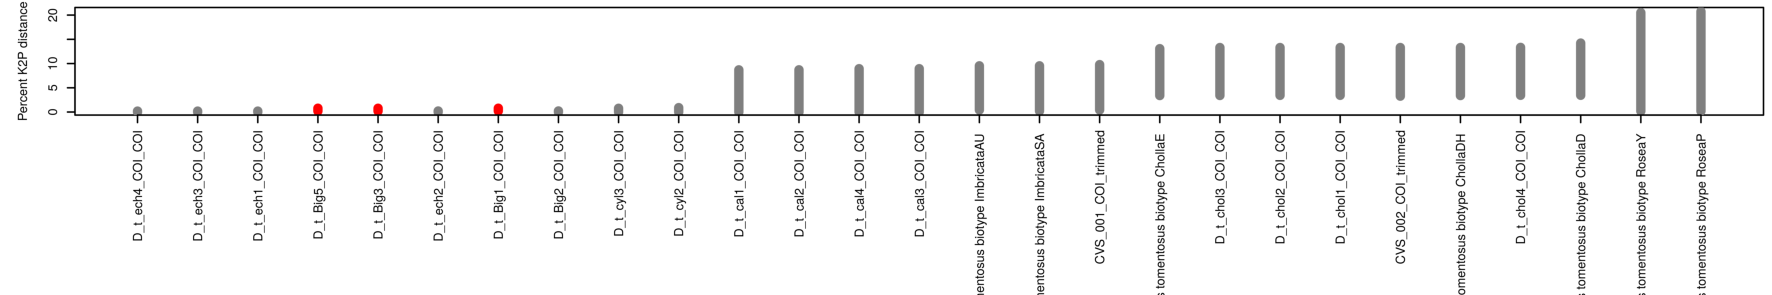
\includegraphics[scale =0.58]{Images/barcodeGap_COIDTOM2.pdf}
% 	\caption{Barcode gaps for DTOMf \& HCO2198 at the lineage (\textit{D. tomentosus}) level.} 
% 	\label{fig:COIDTOM_barcodeGap}
% \end{figure}

\section{ISSR results}

\subsection{Electropherograms}

% \begin{figure}[H]
% 	\centering
% 	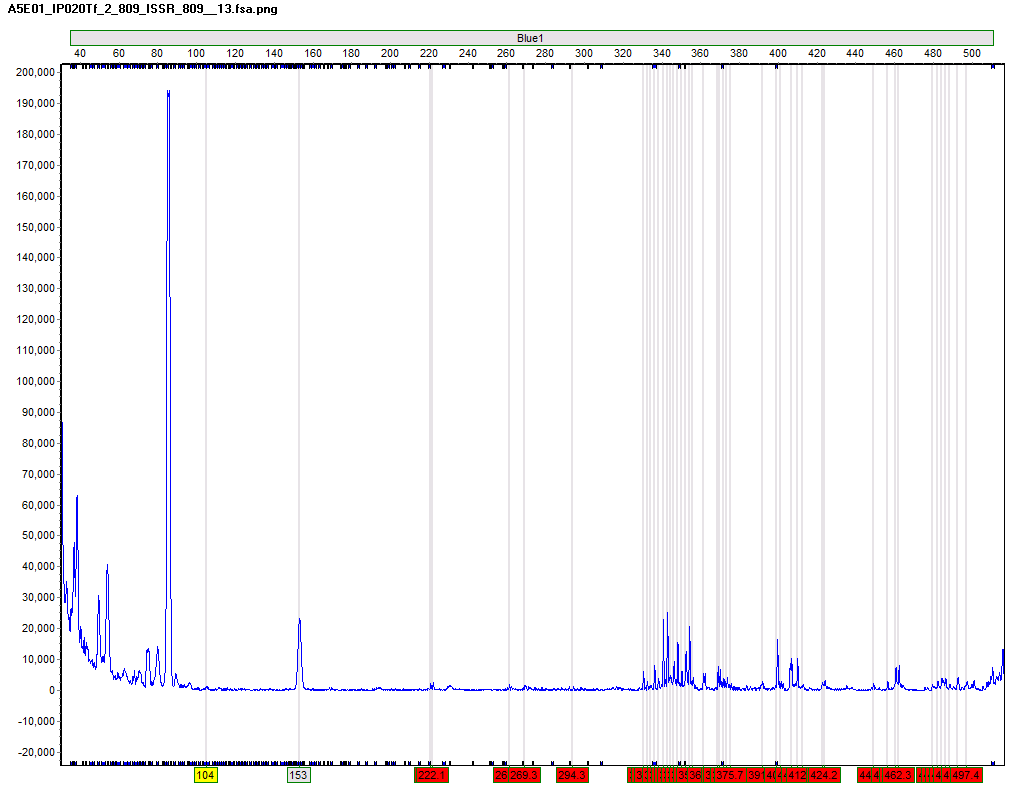
\includegraphics[scale = 0.41]{Images/Tf_electro.png}
%     \newline
% 	\caption{Processed electropherogram for a \textit{Dactylopius tomentosus} `cholla' ISSR sample labelled with 6-FAM\textsuperscript{TM} fluorescent dye. The y-axis represents Relative Fluorescence Units (RFU), and the x-axis displays fragment size in base pairs. Vertical grey lines are peak calls made by GeneMarker\textsuperscript{\textregistered} based on the selected analysis settings.} 
% 	\label{fig:Tf_electro}
% \end{figure}

\begin{figure}[H]
	\centering
	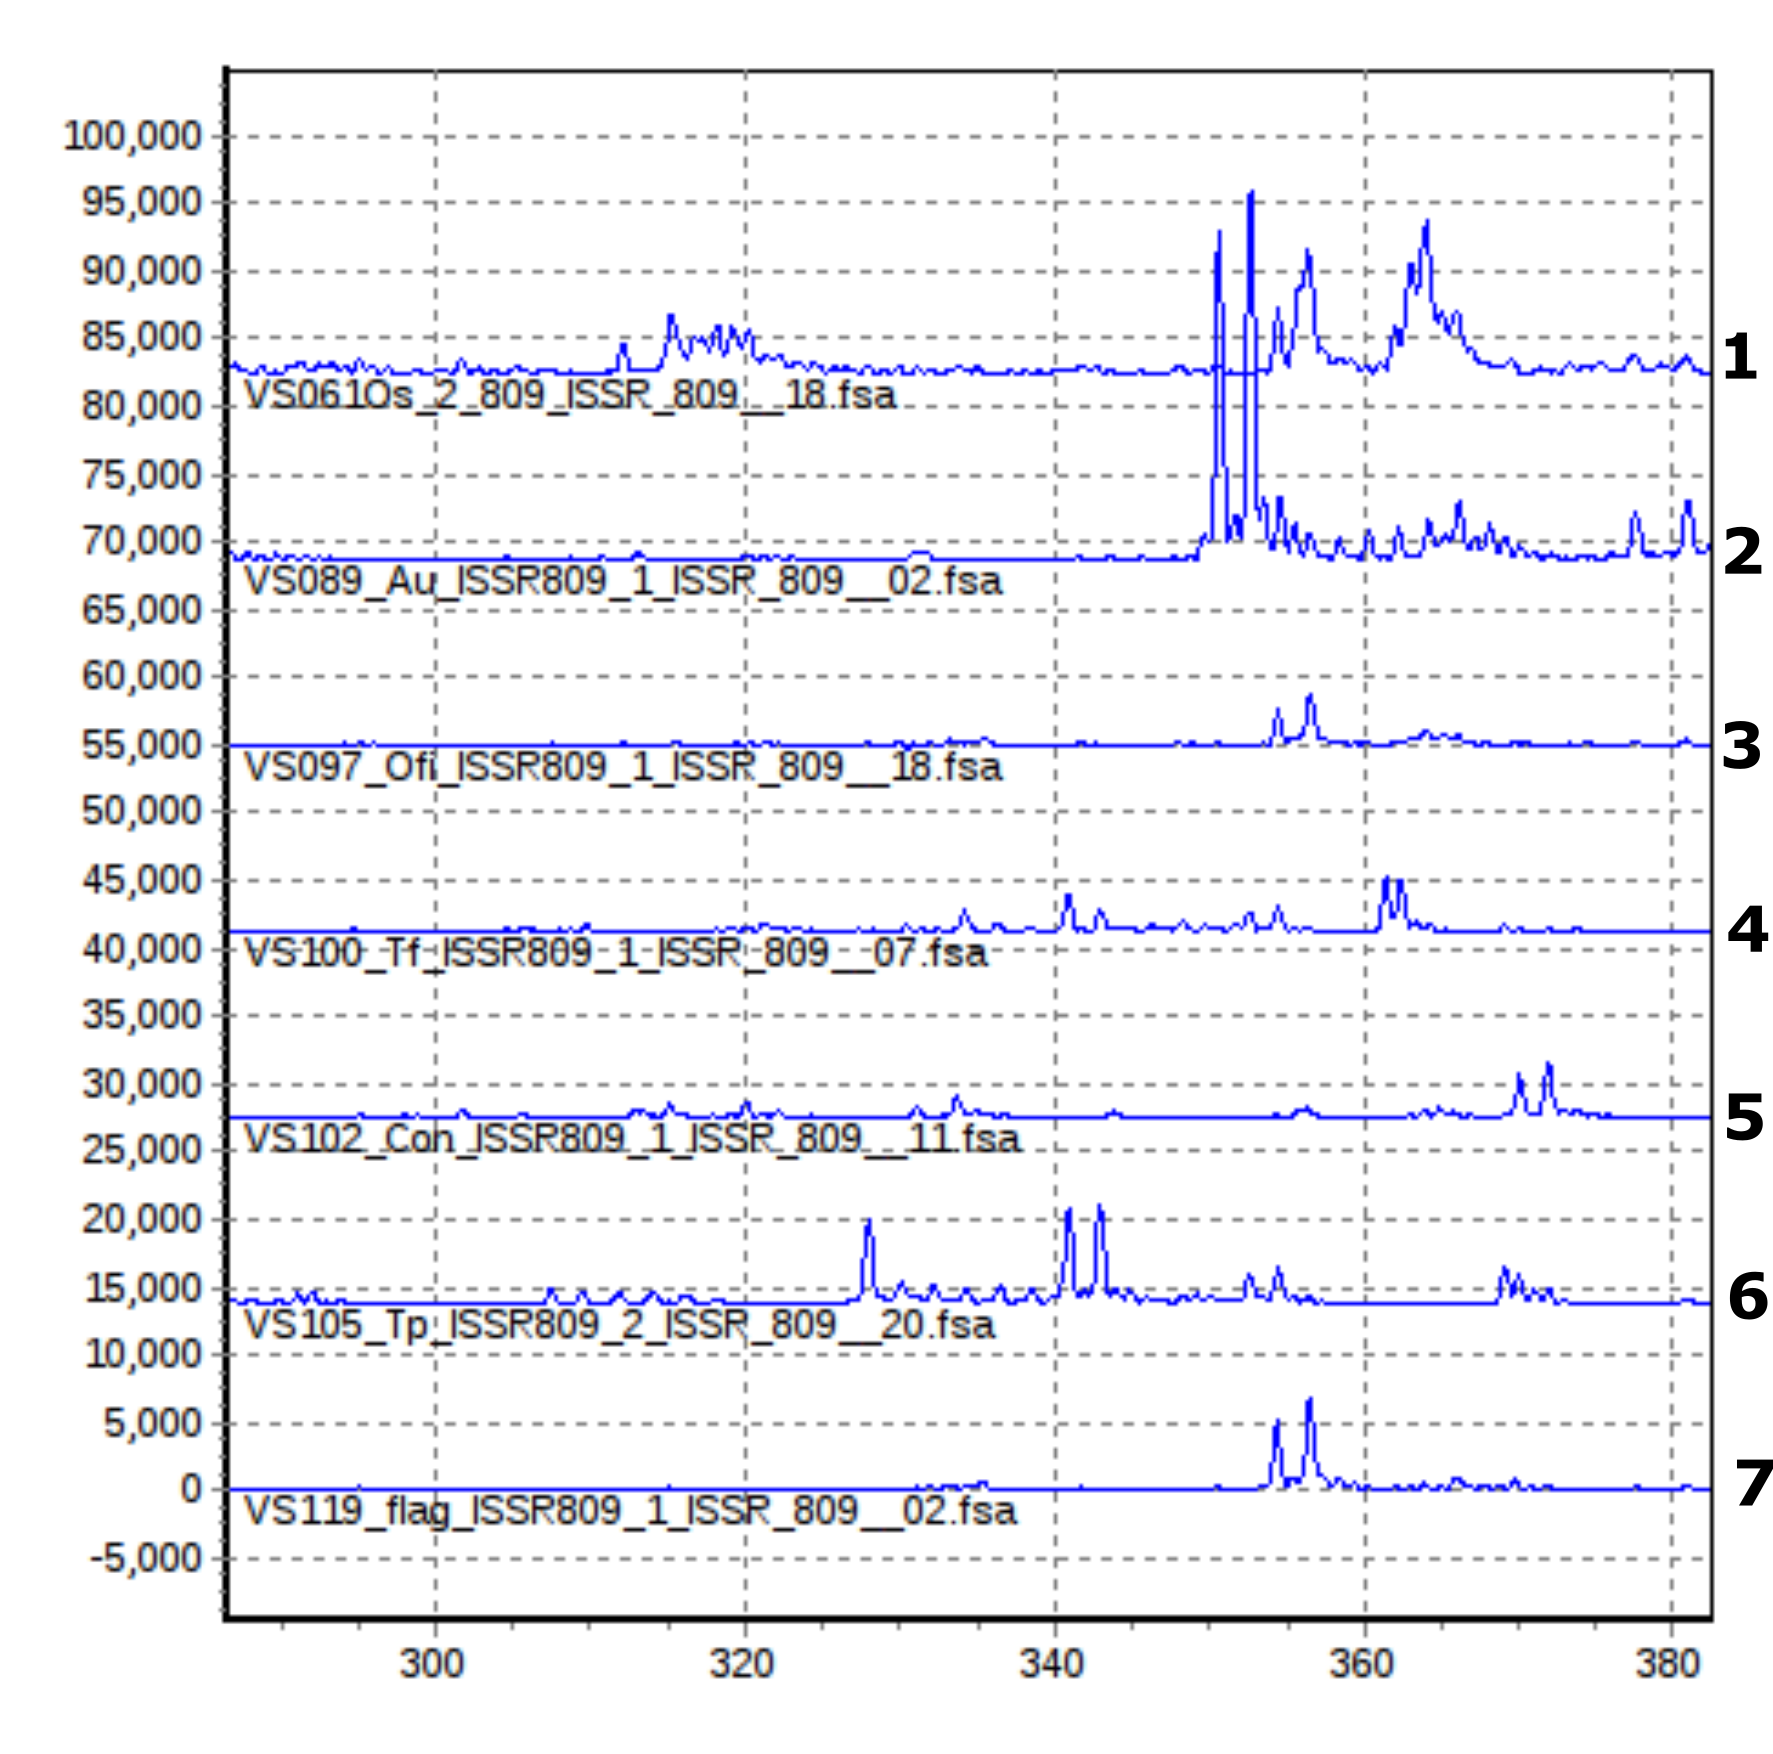
\includegraphics[scale = 1]{Images/overlay_electrophero.png}
	\caption{An overlay view of fragment sizes between 300 and 380 bp for samples (1) \textit{Dactylopius opuntiae} `stricta', (2) \textit{D. austrinus}, (3) \textit{D. opuntiae} `ficus-indica', (4) \textit{D. tomentosus} `cholla', (5) \textit{D. confusus}, (6) \textit{D. tomentosus} `pallida' and (7) \textit{D. opuntiae} collected from Flagstaff (AZ, USA). The y-axis represents Relative Fluorescence Units (RFU), and the x-axis displays fragment size in base pairs.} 
	\label{fig:overlay_electro}
\end{figure}

\subsection{Error rates}
\begin{figure}[H]
	\centering
	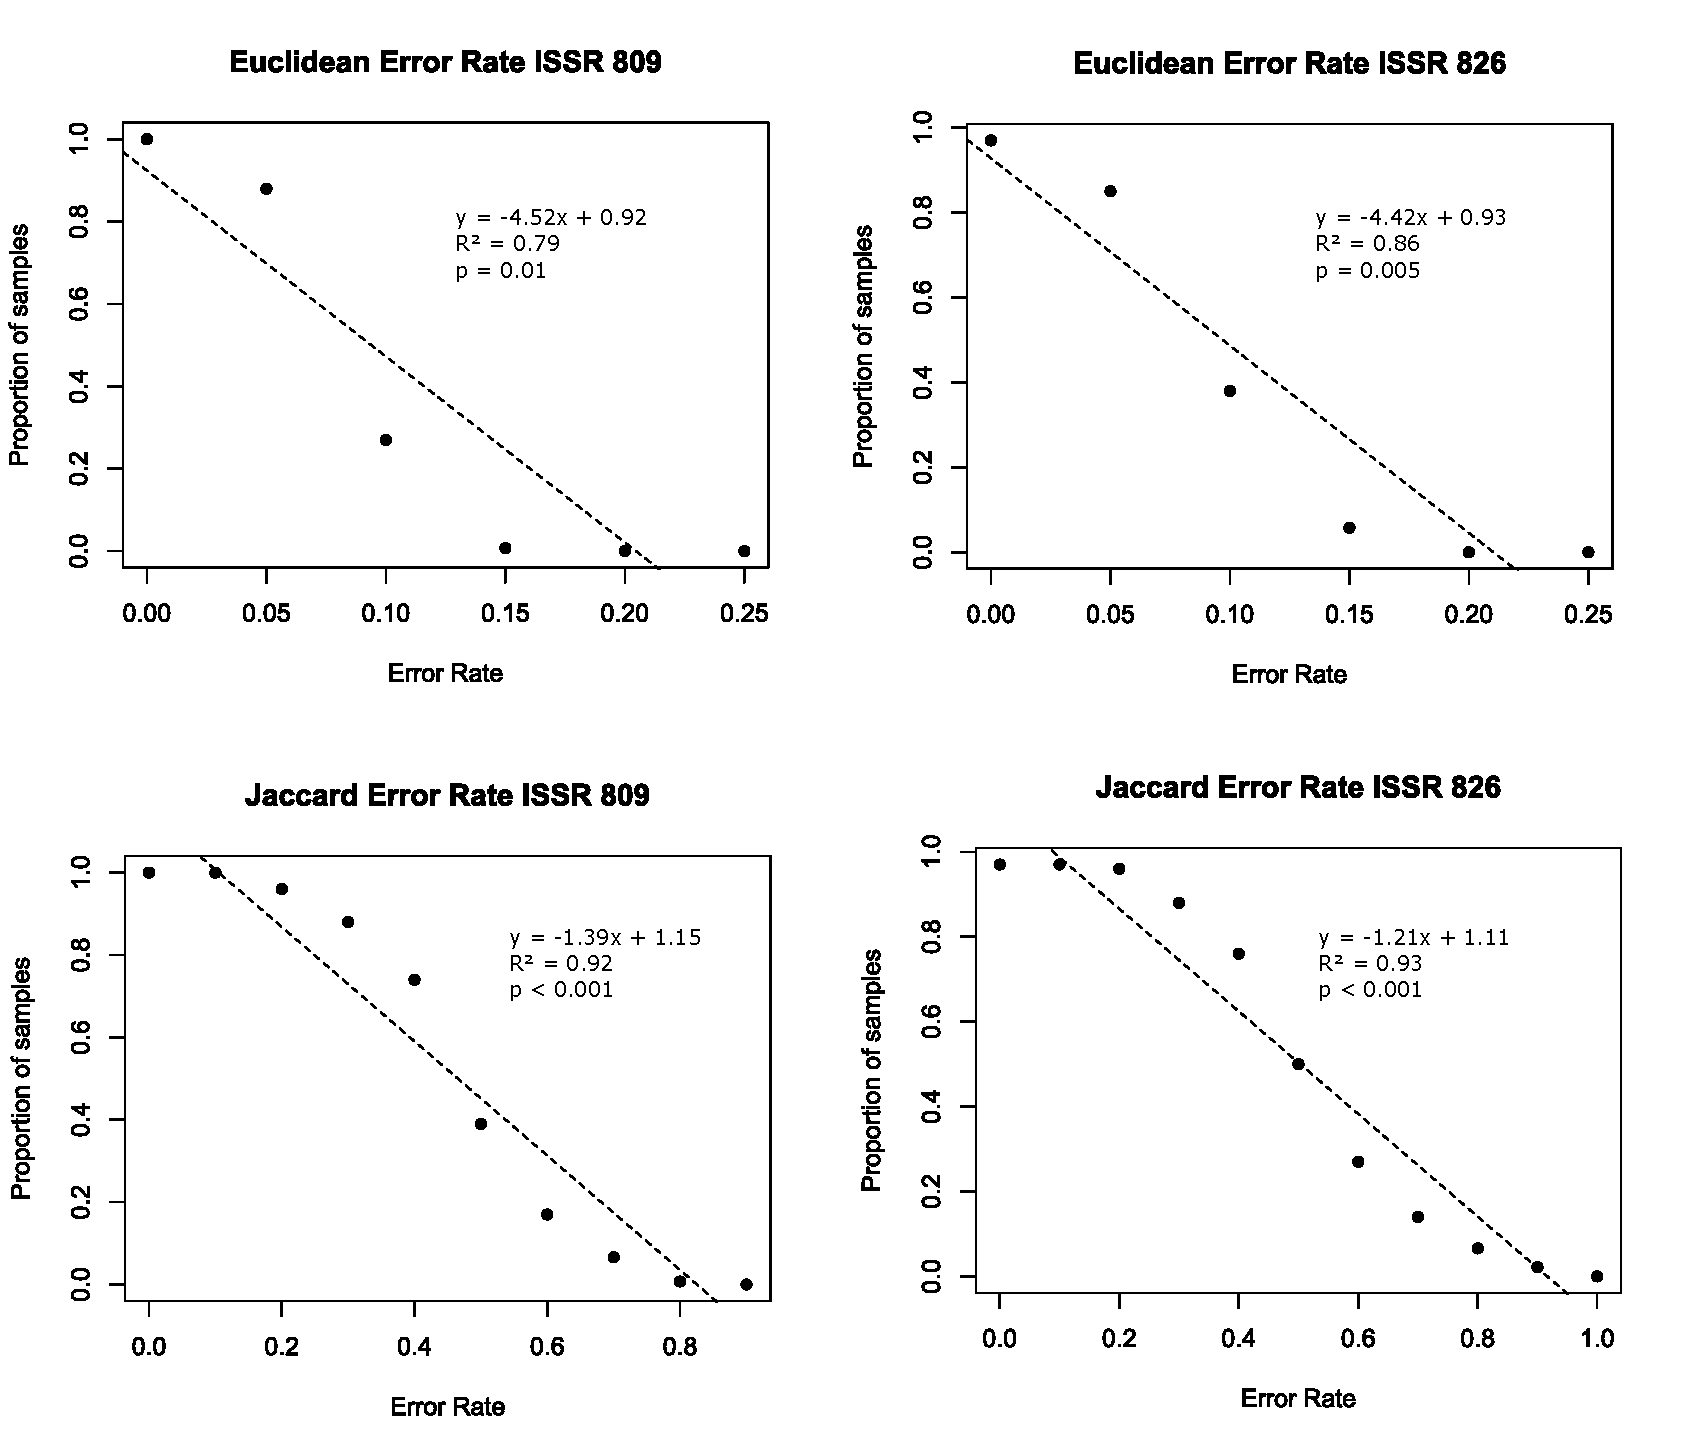
\includegraphics[scale =0.6]{Images/error_rates_graphs.pdf}
	\caption{Euclidean and Jaccard error rates for ISSR primers 826 and 809, showing the proportion of samples greater than a particular error rate. Values are representative of the full data set.}
	\label{fig:error_graphs}
\end{figure}

\begin{figure}[H]
	\centering
	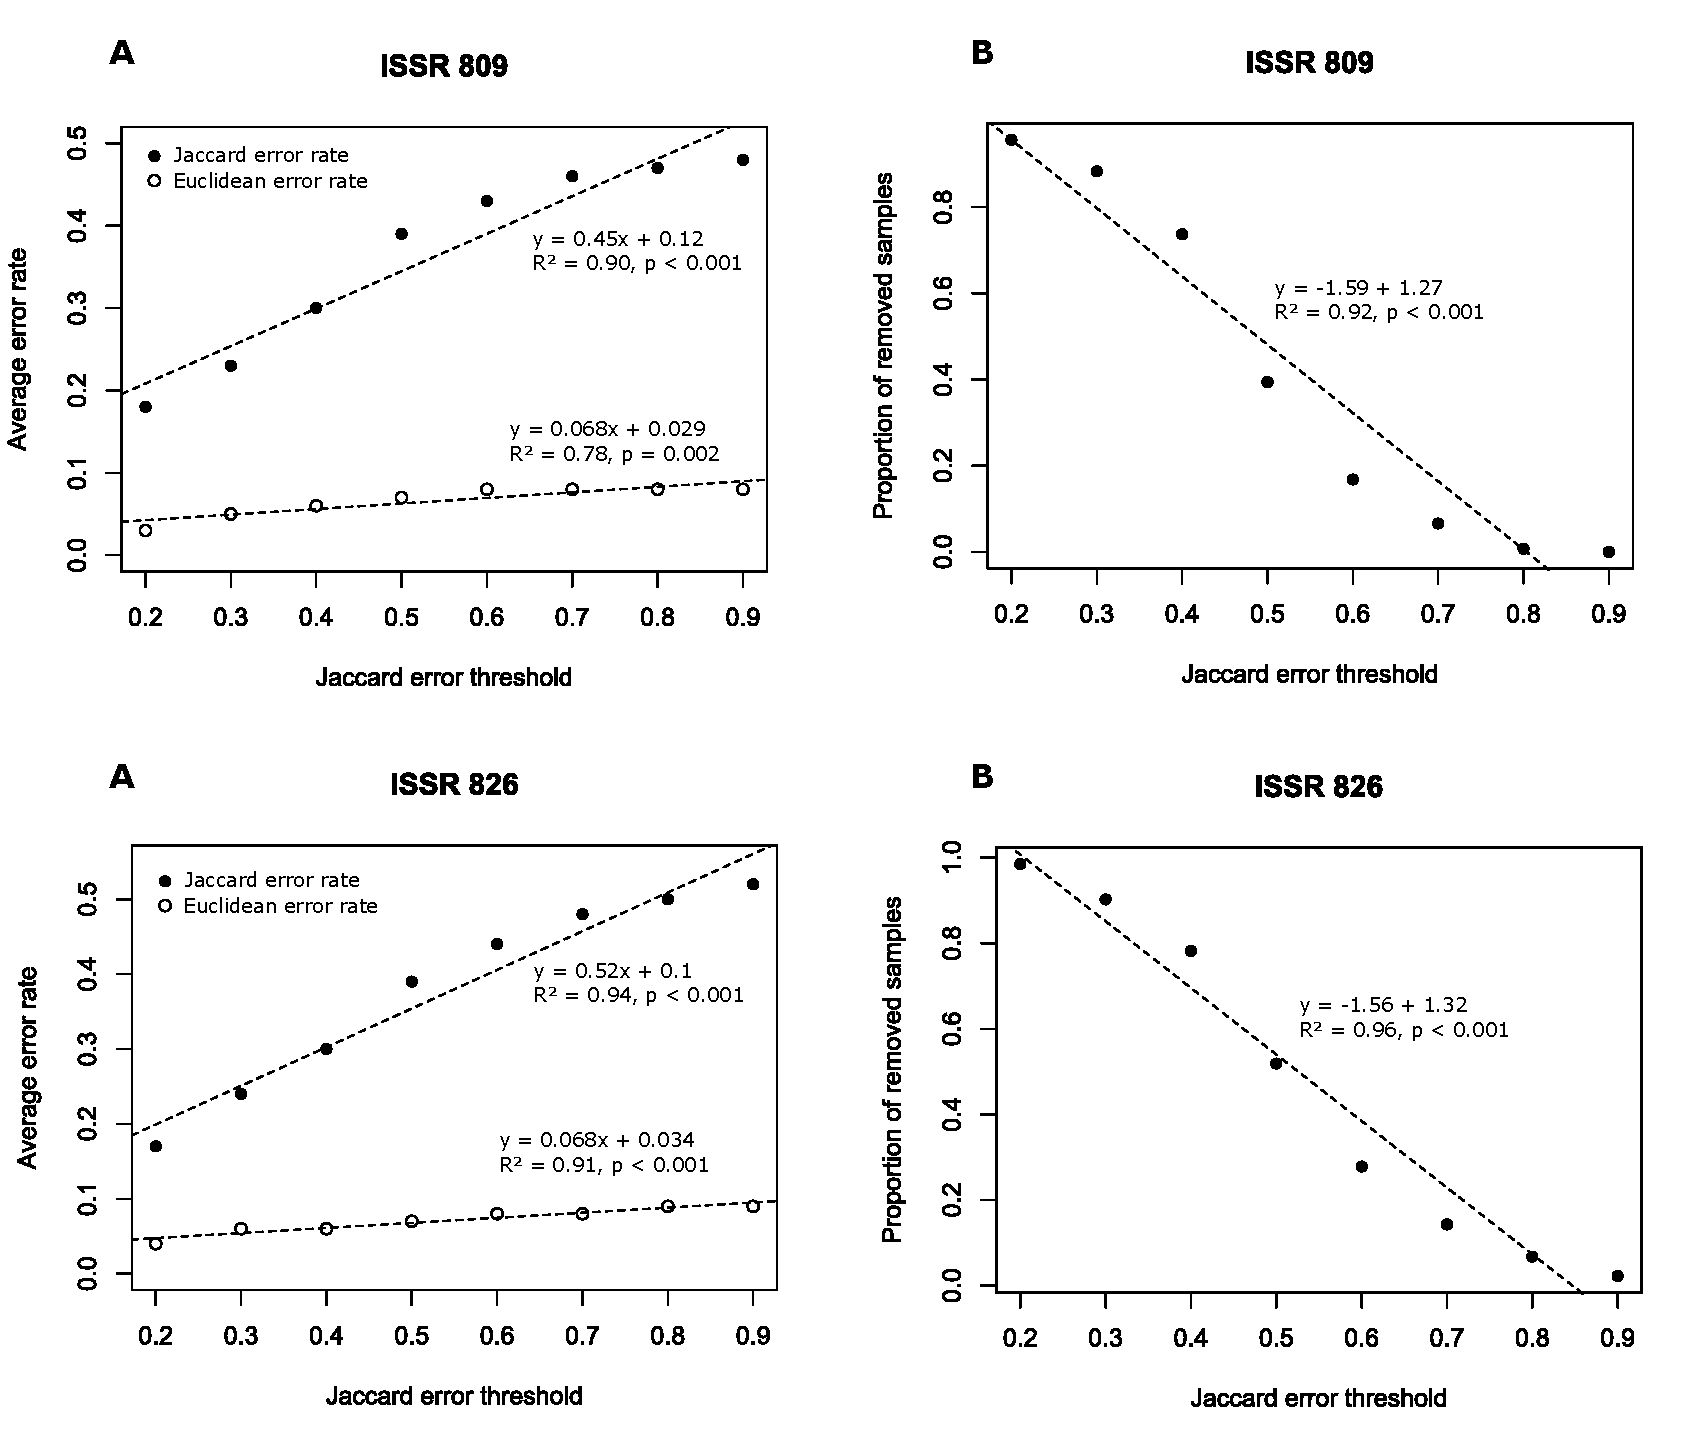
\includegraphics[scale =0.6]{Images/error_stats_graphs.pdf}
	\caption{Graphical representations of the effect of the removal of samples (ISSR 809 and ISSR 826) with a Jaccard error rate greater than a specific threshold on A) the average Jaccard and Euclidean error rates and B) the proportion of removed samples from the data set.}
	\label{fig:error_graphs2}
\end{figure}



\begin{landscape}
\subsection{Splitstree}
\label{appendix:issrSplitstrees}

\begin{figure}[H]
	\centering
	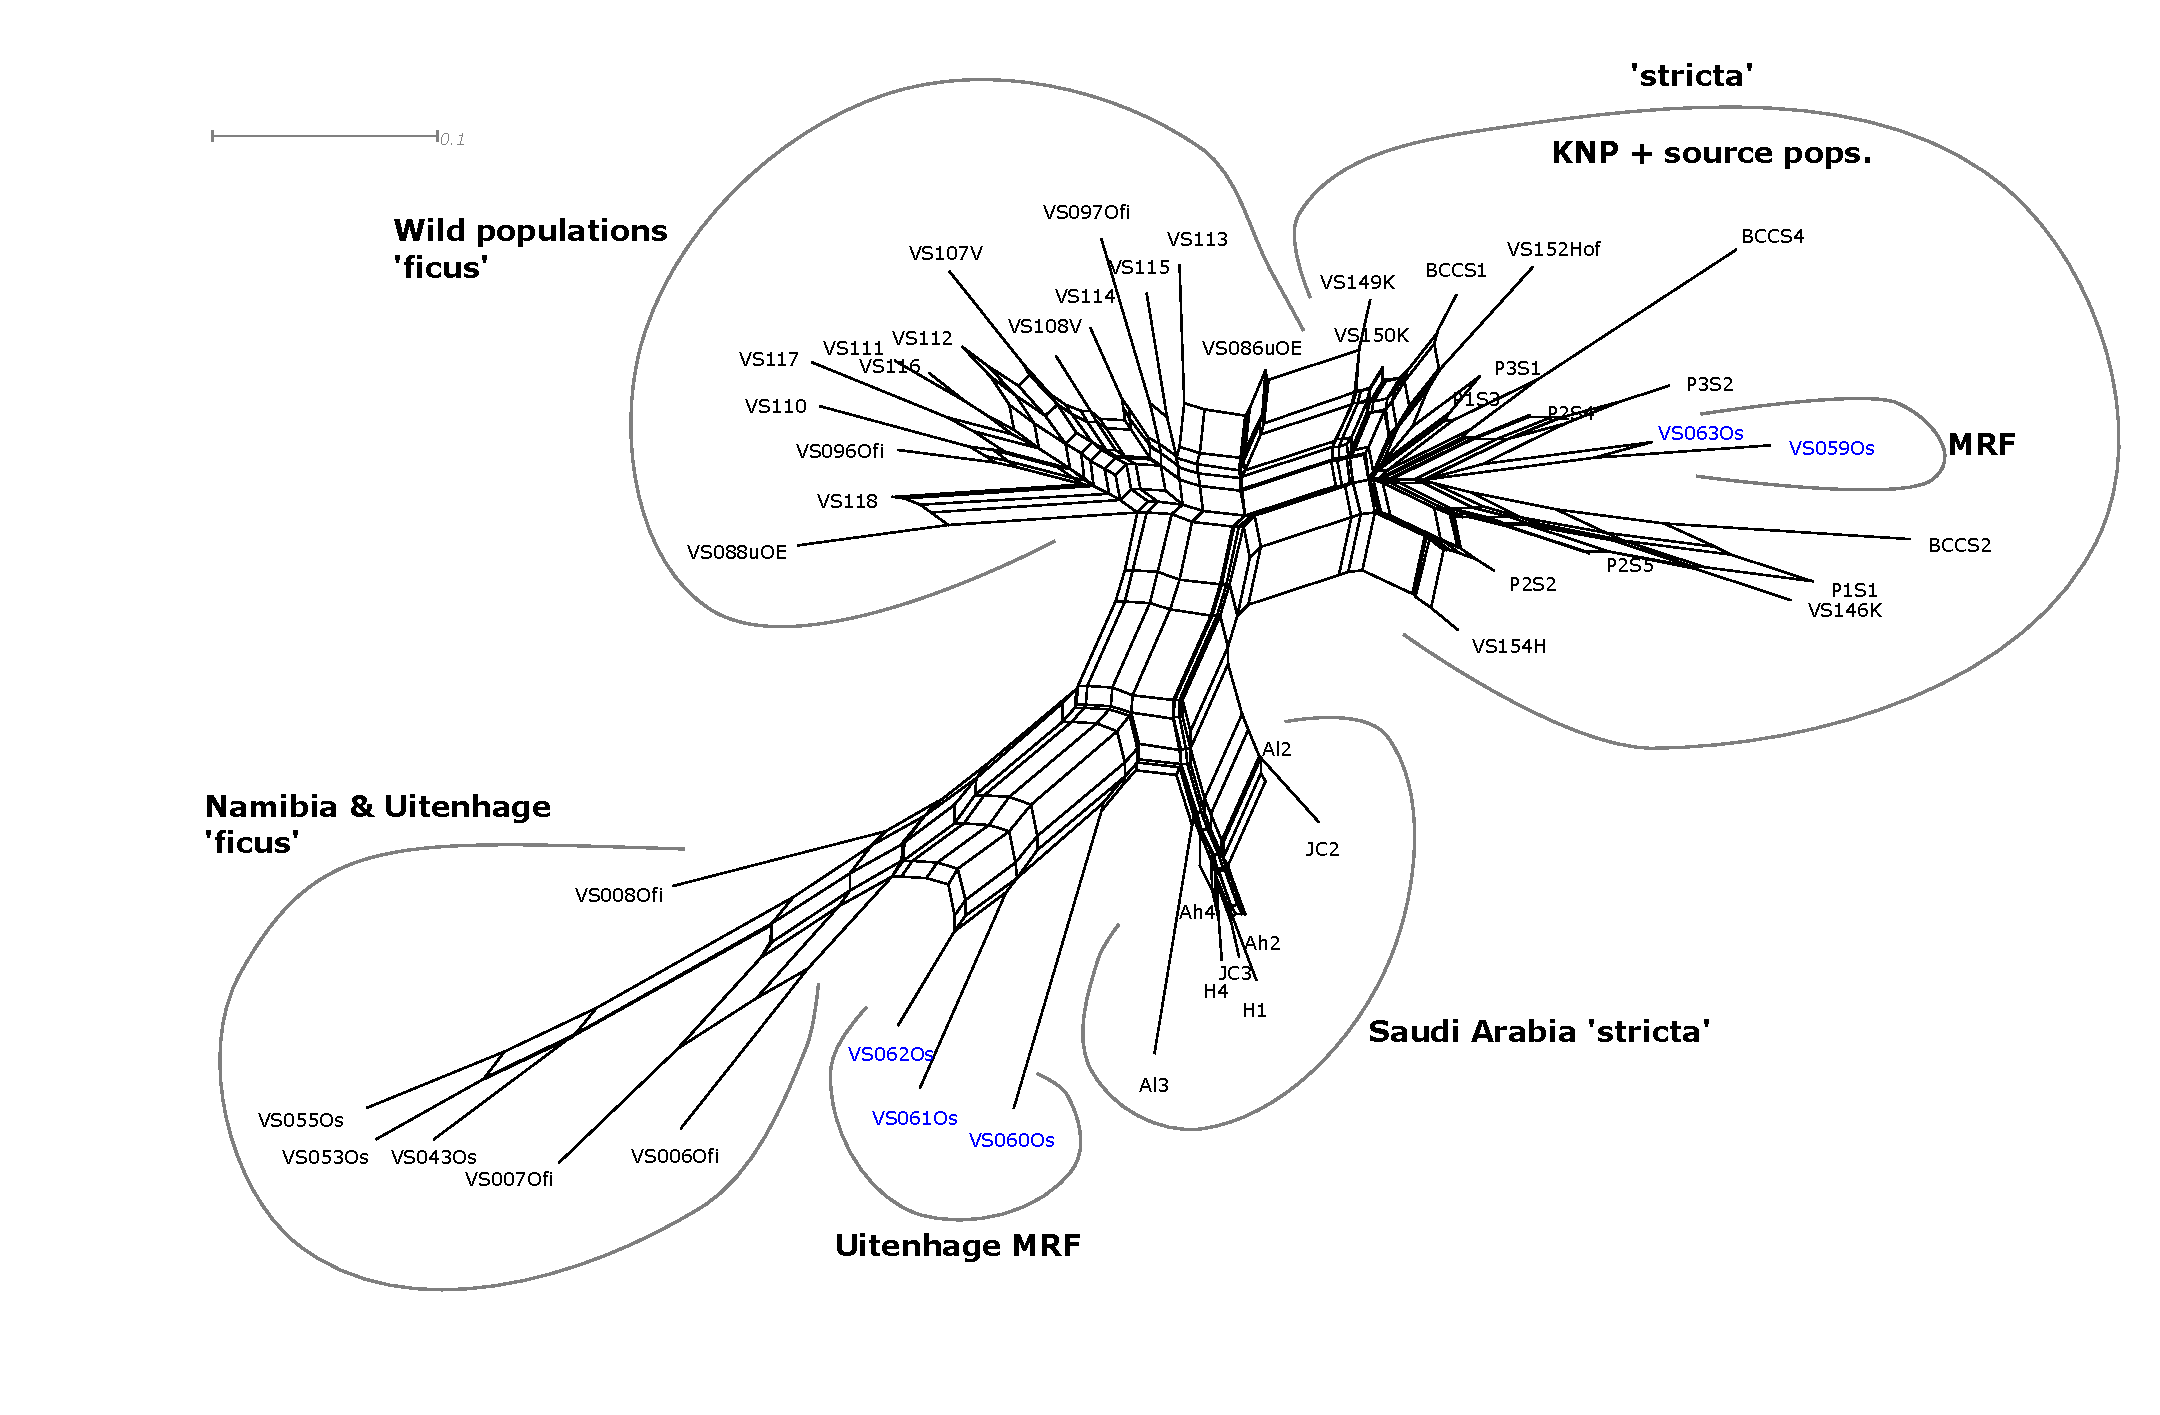
\includegraphics[scale =0.6]{Images/issr809_splitstree.pdf}
	\caption{Splitstree diagram representative of ISSR 809 only. Mass Rearing Facility (MRF) samples are shown in blue. KNP = Kruger National Park, and source pops. = the `stricta' culture kept by Hildegard Klein and John Hoffmann.} 
	\label{fig:issr809_splitstree}
\end{figure}
\end{landscape}


\begin{figure}[H]
	\centering
	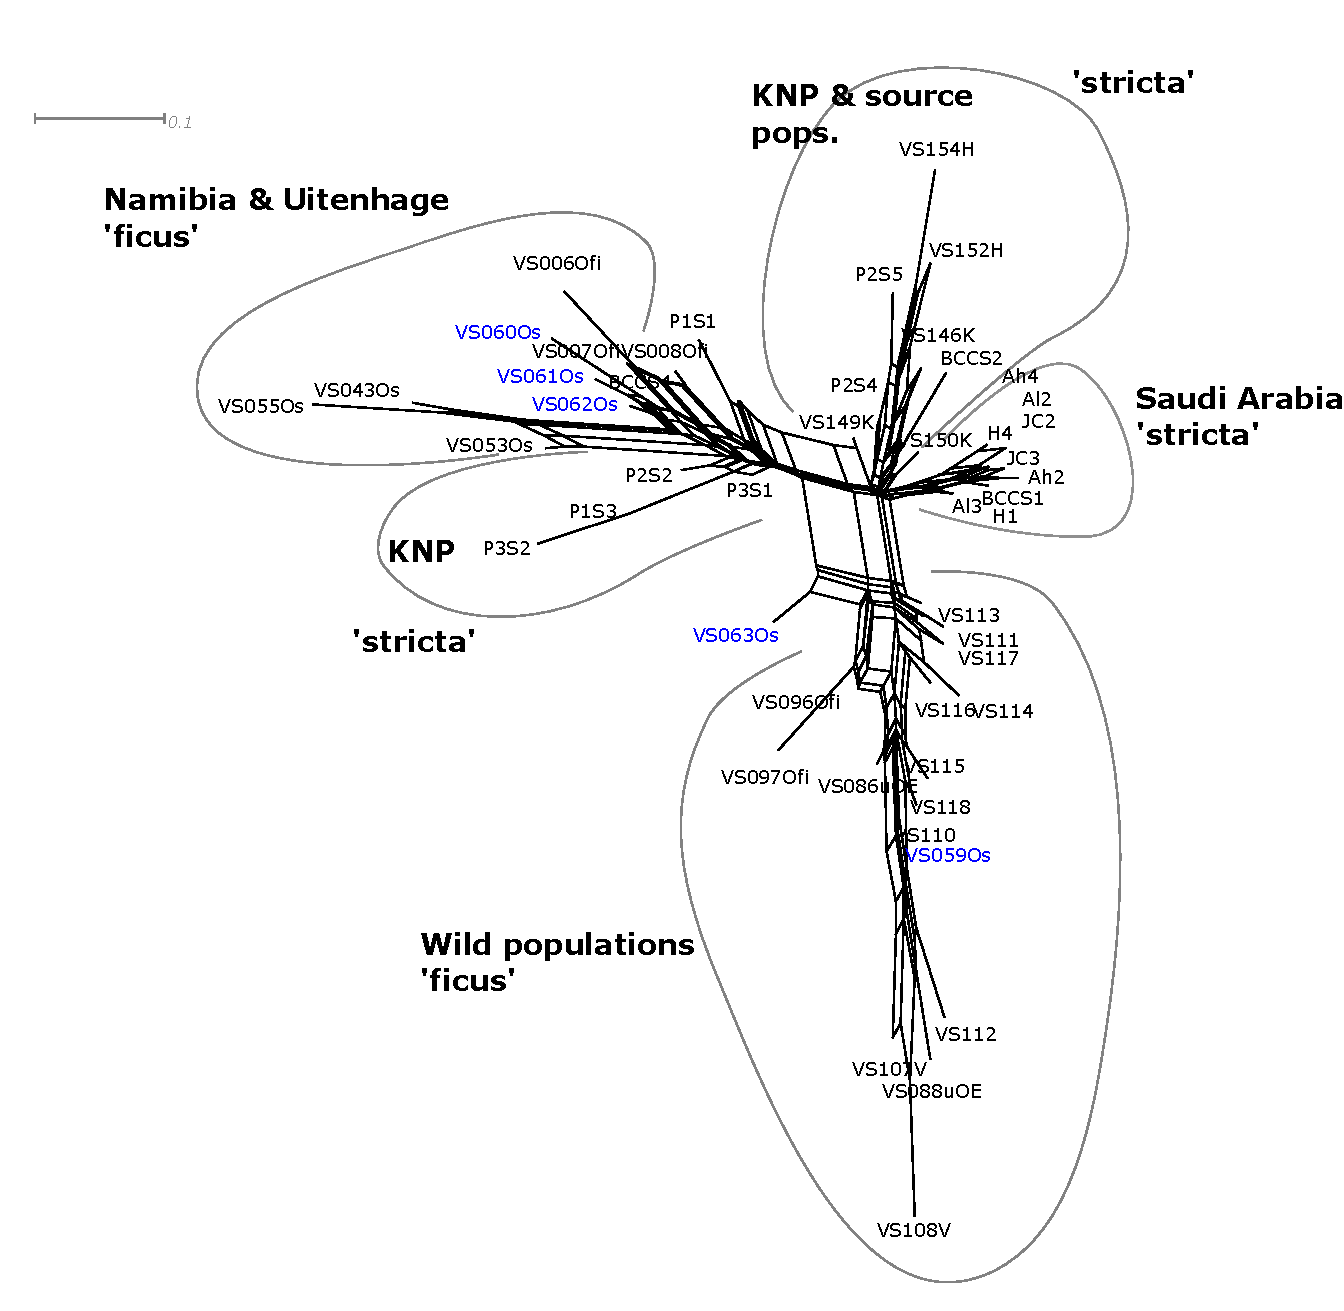
\includegraphics[scale =0.6]{Images/issr826_splitstree.pdf}
	\caption{Splitstree diagram representative of ISSR 826 only. Mass Rearing Facility (MRF) samples are shown in blue. KNP = Kruger National Park, and source pops. = the `stricta' culture kept by Hildegard Klein and John Hoffmann.} 
	\label{fig:issr826_splitstree}
\end{figure}

\begin{landscape}
\subsection{Shepard and scree plots}
\begin{figure}[H]
	\centering
	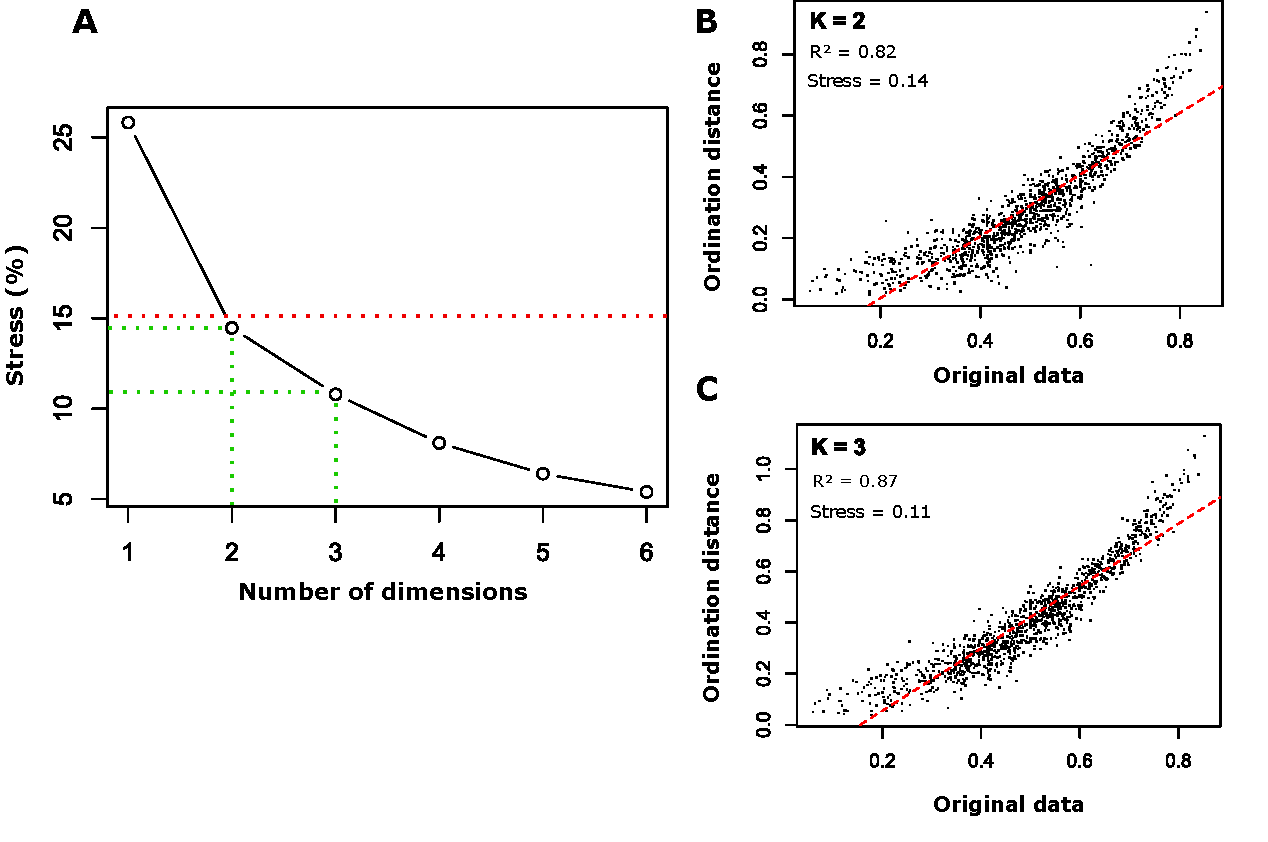
\includegraphics[scale =0.9]{Images/scree_and_shepard_plots.pdf}
	\caption{A) Scree plot showing the relationship between the number of dimensions used for a non-metric MDS, and the corresponding stress score. Stress scores below 15\% are considered to be a good fit for the data (indicated by the dashed red line). Stress scores for K = 2 and K = 3 are indicated by the dashed green lines. Shepard plots are shown in B) (K = 2) and C) (K = 3), plotting the relationship between the original distance data and the distances resulting from the ordination transformation. A high R\textsuperscript{2} value is desirable, as that indicates an accurate reflection of the data in the ordination plot.} 
	\label{fig:shep_plots}
\end{figure}
\end{landscape}

% \subsection{Structure results}
% \begin{figure}[H]
% 	\centering
% 	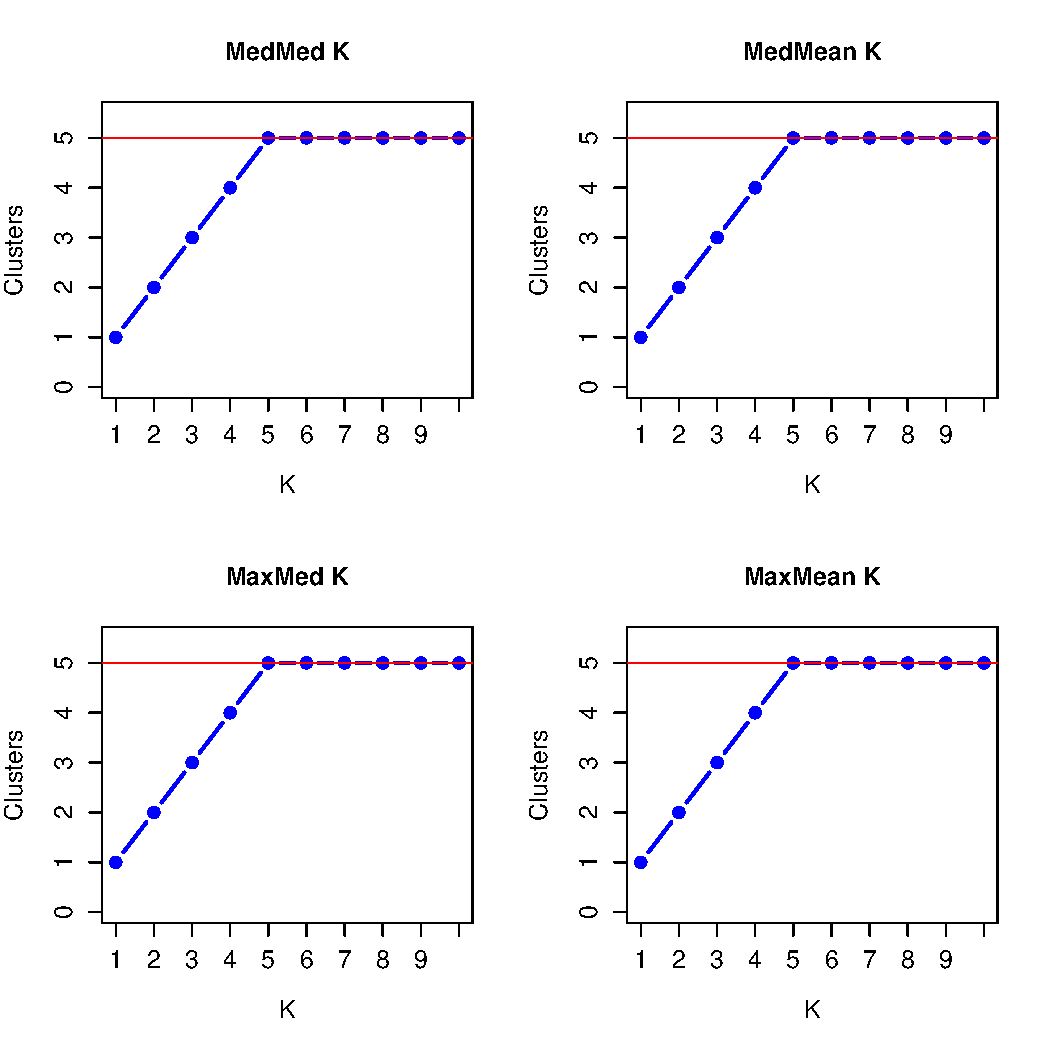
\includegraphics[scale =0.7]{Images/MedK_0,7_without_priors.pdf}
% 	\caption{Estimation of the optimal \textit{K}-value (\textit{K} = 5) according to the four methods presented by \citet{puechmaille2016program}. The threshold value presented above was set to 0.6. (PopData was not set as a prior).}
% 	\label{fig:struc_thresh0.6}
% \end{figure}

% \begin{figure}[H]
% 	\centering
% 	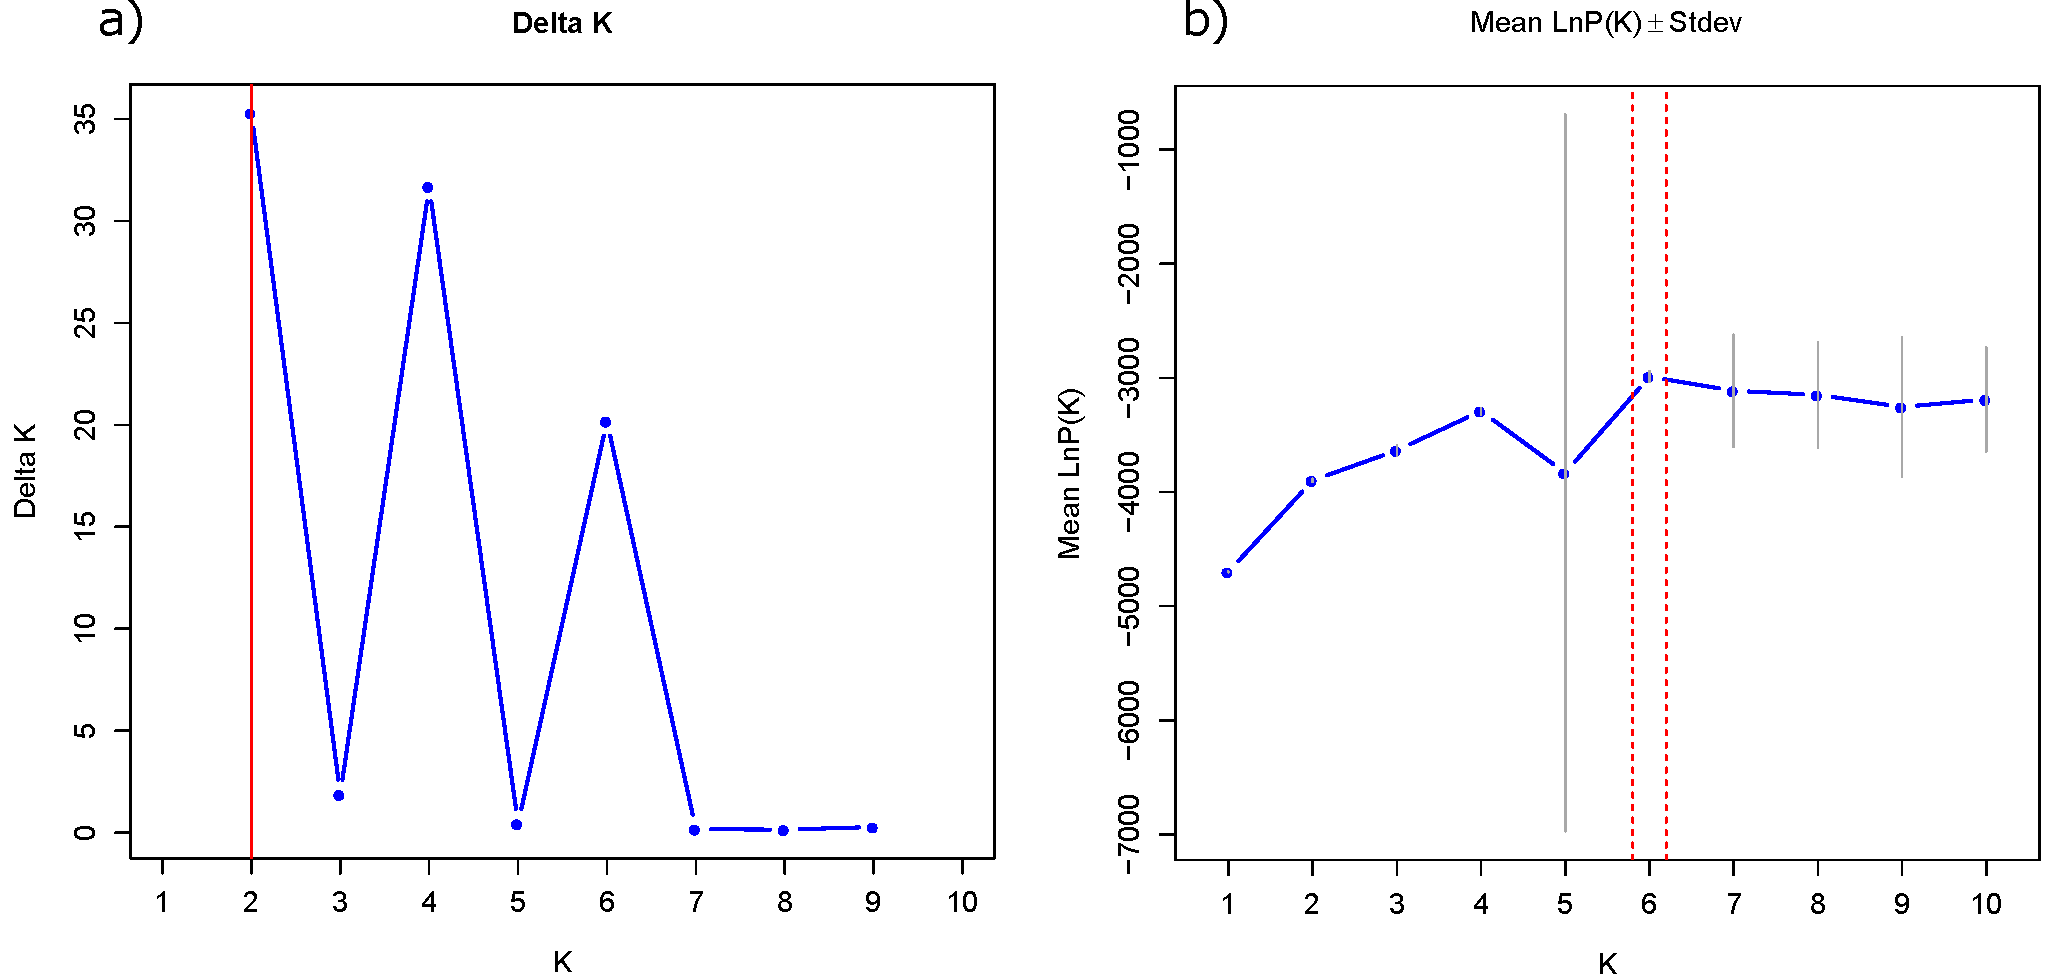
\includegraphics[scale =0.45]{Images/DeltaK_LnPK_without_priors.pdf}
% 	\caption{Estimation of the optimal \textit{K}-value, using a) $\Delta$\textit{K} and b) the mean LnP(\textit{K}) estimates as per the methods of \citet{evanno2005detecting}. (PopData was not set as a prior).}
% 	\label{fig:struc_evanno}
% \end{figure}

% \begin{figure}[H]
% 	\centering
% 	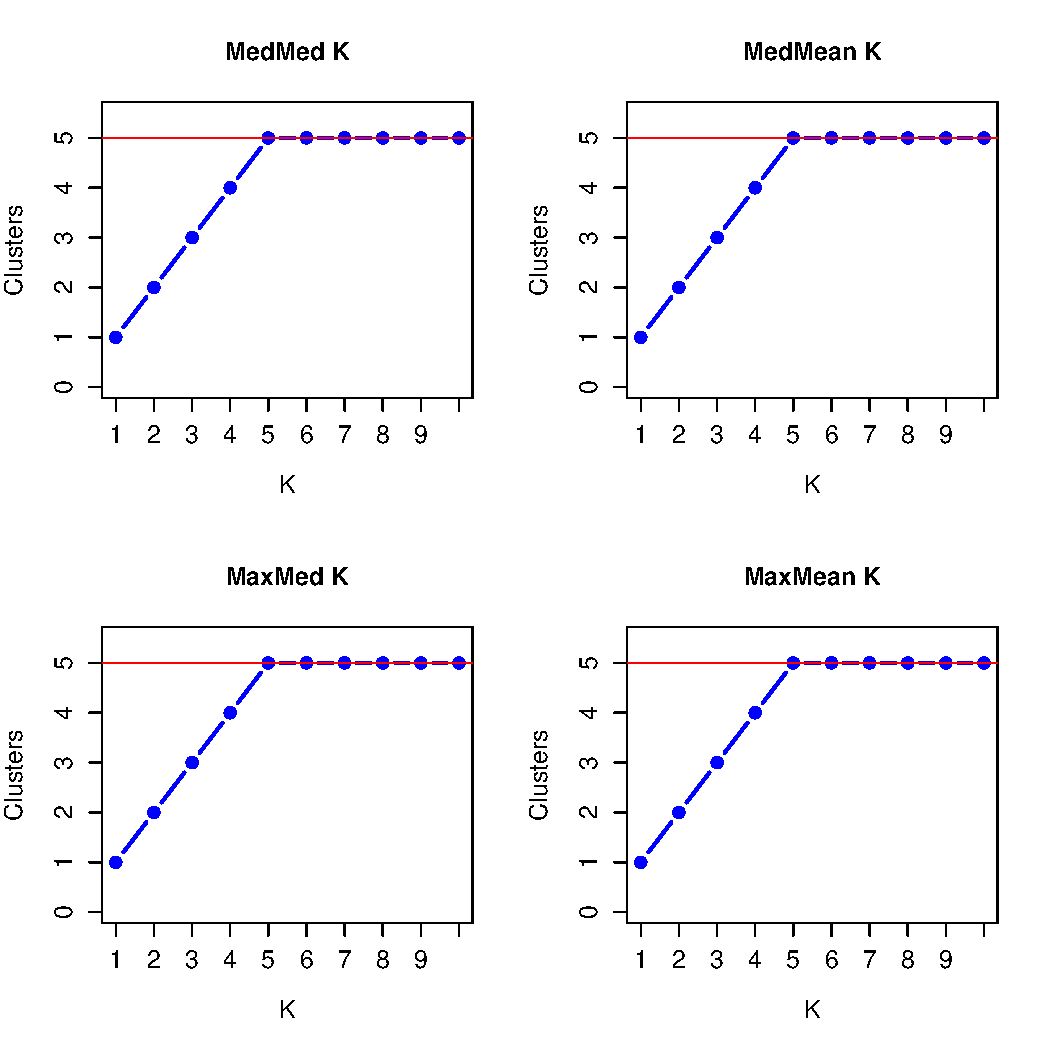
\includegraphics[scale =0.7]{Images/with_priors_structure_medK_graphs.pdf}
% 	\caption{Estimation of the optimal \textit{K}-value (\textit{K} = 5) according to the four methods presented by \citet{puechmaille2016program}. The threshold value presented above was set to 0.7. PopData set as a prior.}
% 	\label{fig:struc_K_locprior_puech}
% \end{figure}

% \begin{figure}[H]
% 	\centering
% 	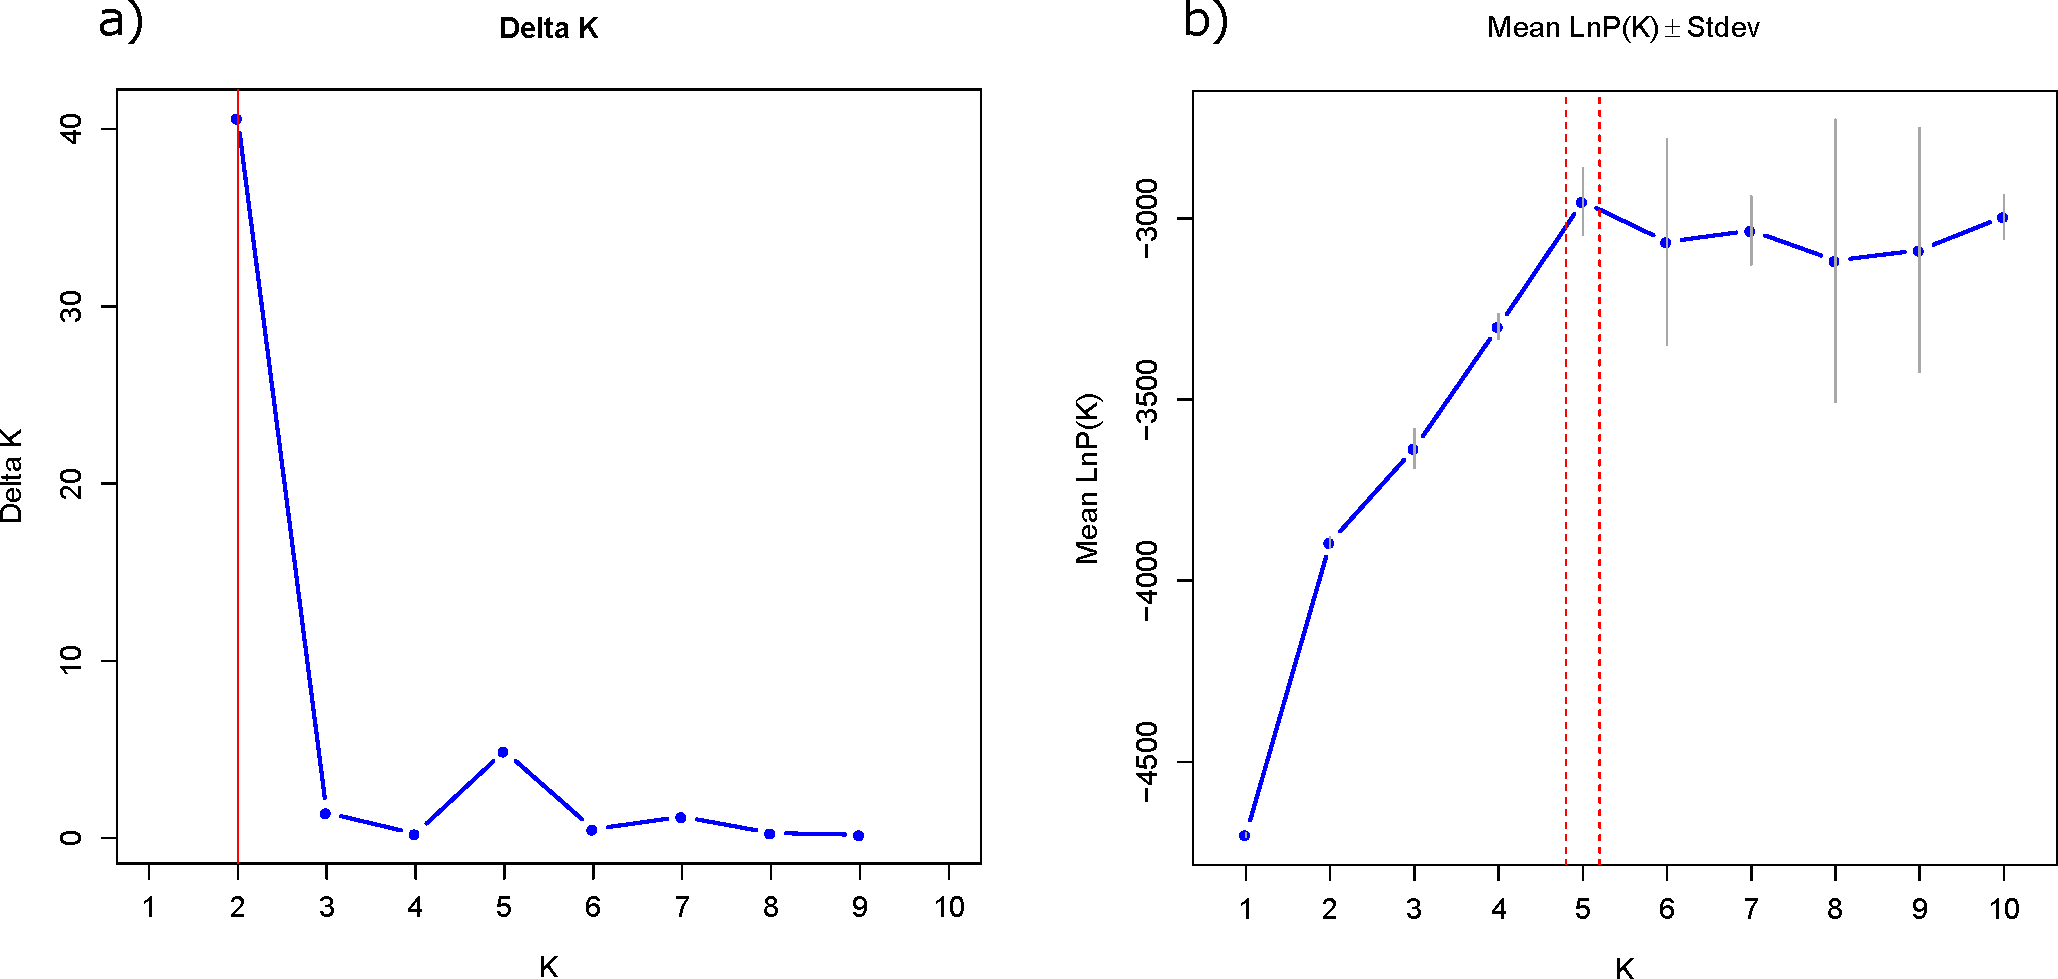
\includegraphics[scale =0.45]{Images/DeltaK_LnPK.pdf}
% 	\caption{Estimation of the optimal \textit{K}-value, using a) $\Delta$\textit{K} and b) the mean LnP(\textit{K}) estimates as per the methods of \citet{evanno2005detecting}. PopData set as a prior.}
% 	\label{fig:struc_locprior_evanno}
% \end{figure}

\subsection{ISSR primer statistics}
\begin{table}[H]
\caption{POPGENE statistical output for each individual primer and their concatenation for the `stricta' and `ficus' genetic clusters. na = number of alleles, ne = effective number of alleles, h = Nei's genetic diversity, I = Shannon's information index, No. PM loci = number of polymorphic loci, \% PM loci = percentage polymorphic loci, Ht = total genetic diversity, Hs = intra population genetic diversity,  Gst = coefficient of gene differentiaion. All values presented are averages. For the intra-group statistics, Saudi Arabia + Kruger N. Park + Klein \& Hoffmann = `stricta', and Uitenhage + Namibia + wild populations = `ficus'.}
\label{tab:issr_stats_eachPrimer}
\renewcommand{\arraystretch}{0.5}
\resizebox{\columnwidth}{!}{
\begin{tabular}{@{}llcccccclll@{}}
\toprule
\textbf{Primer} & \textbf{Group} & \textbf{na} & \textbf{ne} & \textbf{h} & \textbf{I} & \textbf{No. PM loci} & \textbf{\%  PM loci} & \textbf{Ht} & \textbf{Hs} & \textbf{Gst} \\ \midrule
\textbf{ISSR 809} & stricta & 1.20 & 1.09 & 0.06 & 0.09 & 78 & 20.31 & 0.06 & 0.03 & 0.51 \\
 & ficus & 1.41 & 1.17 & 0.11 & 0.17 & 156 & 40.62 & 0.14 & 0.06 & 0.59 \\
 & Mass Rearing Facility & 1.19 & 1.14 & 0.08 & 0.11 & 74 & 19.27 &  &  &  \\
 & All & 1.45 & 1.15 & 0.10 & 0.16 & 174 & 45.31 & 0.13 & 0.10 & 0.23 \\
 & \textbf{INTRA-GROUP:} &  &  &  &  &  &  &  &  &  \\
 & Saudi Arabia & 1.08 & 1.05 & 0.03 & 0.04 & 30 & 7.81 &  &  &  \\
 & Kruger N. Park & 1.09 & 1.06 & 0.03 & 0.05 & 35 & 9.11 &  &  &  \\
 & Klein \& Hoffmann & 1.07 & 1.05 & 0.03 & 0.04 & 27 & 7.03 &  &  &  \\
 & Uitenhage & 1.15 & 1.13 & 0.07 & 0.10 & 56 & 14.58 &  &  &  \\
 & Namibia & 1.12 & 1.11 & 0.06 & 0.08 & 47 & 12.24 &  &  &  \\
 & Wild populations & 1.15 & 1.08 & 0.05 & 0.07 & 58 & 15.1 &  &  &  \\
\textbf{ISSR 826} & stricta & 1.03 & 1.03 & 0.01 & 0.02 & 11 & 3.01 & & & \\
 & ficus & 1.03 & 1.03 & 0.02 & 0.02 & 12 & 3.28 & & &  \\
 & stricta + ficus & 1.06 & 1.04 & 0.03 & 0.04 & 23 & 6.28 & & &  \\ 

 \bottomrule
\end{tabular}
}
\end{table}

% \subsection{POPGENE file input}
% \label{appendix:popgene_input}

% The POPGENE input file followed the following format, where a `.' indicates missing or ambiguous data: \newline

% \noindent /*ISSRpopgene*/ \\
% Number of populations = 2 \\
% Number of loci = 6 \\
% locus name: \\
% Locus 1 Locus 2 Locus 3 Locus 4 Locus 5 Locus 6\\

% \noindent name = population1 \\
% 001110 \\
% 001110 \\
% 0110.0 \\
% 11001. \\

% \noindent name = population2 \\
% 0.0111 \\
% 010111 \\
% 0.1110 \\
% 1110.1 \\

\subsection{Genetic distance and diversity}
All \textit{D. opuntiae} specimens showed an average Jaccard distance of 0.48 (SE $\pm$ 0.01) (Fig. \ref{fig:genetic_distances_boxplot}). None of the within-group genetic distances showed significant differences (Kruskal-Wallis ANOVA: Fig. \ref{fig:genetic_distances_boxplot}A)  Chi-square = 2.84, p= 0.24, and Fig. \ref{fig:genetic_distances_boxplot}B) Chi-square = 6.72, p= 0.081).
By group, `ficus' had the highest percentage of polymorphic loci (PM) (38.53 \%), as well as genetic diversity (h = 0.10, I = 0.16), while samples from the MRF had the lowest percentage PM loci (17.33 \%) (Table \ref{tab:popgene_stats}). \\

\begin{figure}[H]
	\centering
	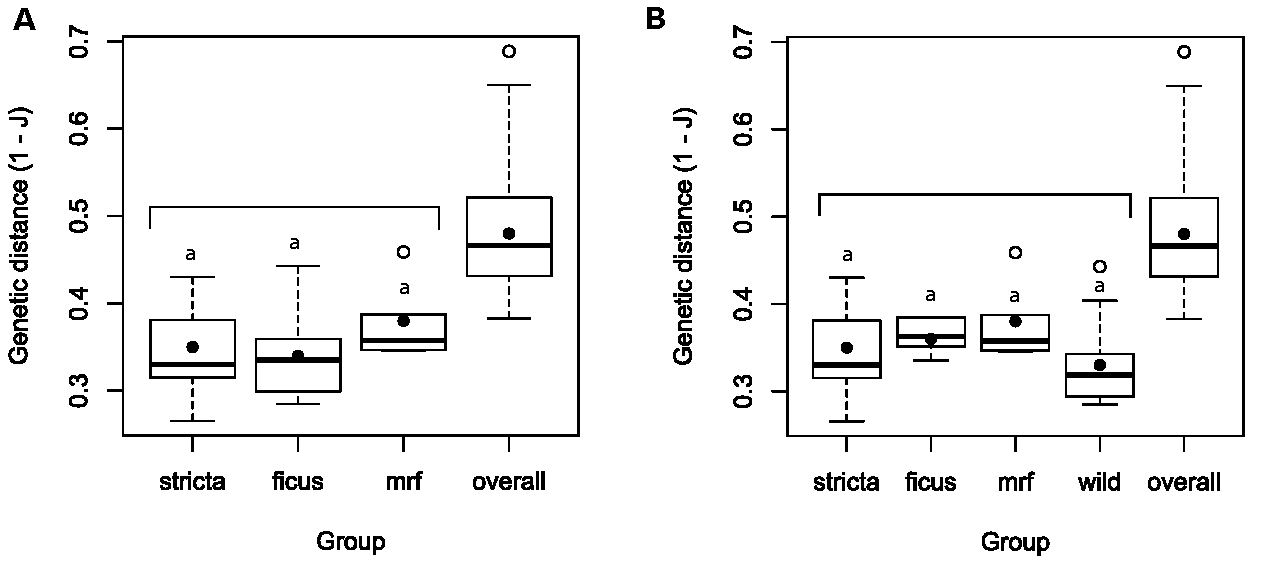
\includegraphics[scale =0.75]{Images/genetic_distances_boxplot.pdf}
	\caption{Box plots for within and overall group genetic distances for \textit{D. opuntiae}, measured by the Jaccard distance (1-J). A) `ficus' taken as a whole and B) wild populations removed from `ficus' and put into its own group. Solid black dots are the means, and the same letters above each box indicate non-significance.}
	\label{fig:genetic_distances_boxplot}
\end{figure}

% At the intra-group level, wild populations (`ficus') had the highest percentage PM loci (14.8\%), and the Hoffmann and Klein `stricta' source populations had the lowest (6.67\%) (Table \ref{tab:popgene_stats}). \\
% The largest genetic distances were between Namibian `ficus' and 1) the Hoffmann and Klein `stricta' source populations (0.189), 2) Kruger National Park `stricta' (0.177), 3) wild population `ficus' (0.173) and 4) Saudi Arabian `stricta' samples (0.168) (Table \ref{tab:popgene_genetic_distances}). 
 
\begin{table}[H]
\renewcommand{\arraystretch}{0.5}
\caption{POPGENE statistical output for the concatenation of ISSR 809 and ISSR 826 for the `stricta' and `ficus' genetic clusters. na = number of alleles, ne = effective number of alleles, h = Nei's genetic diversity, I = Shannon's information index, No. PM loci = number of polymorphic loci, \% PM loci = percentage polymorphic loci, Ht = total genetic diversity, Hs = intra population genetic diversity,  Gst = coefficient of gene differentiaion. All values presented are averages. For the intra-group statistics, Saudi Arabia + Kruger N. Park + Klein \& Hoffmann = `stricta', and Uitenhage + Namibia + wild populations = `ficus'.}
\label{tab:popgene_stats}
\resizebox{\columnwidth}{!}{
\begin{tabular}{@{}llcccccclll@{}}
\toprule
\textbf{Primer} & \textbf{Group} & \textbf{na} & \textbf{ne} & \textbf{h} & \textbf{I} & \textbf{No. PM loci} & \textbf{\%  PM loci} & \textbf{Ht} & \textbf{Hs} & \textbf{Gst} \\ \midrule
 \textbf{ISSR 809 \& ISSR 826} & stricta & 1.22 & 1.10 & 0.06 & 0.10 & 165 & 22 & 0.06 & 0.03 & 0.48 \\
 & ficus & 1.39 & 1.16 & 0.10 & 0.16 & 289 & 38.53 & 0.14 & 0.05 & 0.63 \\
 & Mass Rearing Facility & 1.17 & 1.13 & 0.07 & 0.10 & 130 & 17.33 & & & \\
 & All & 1.45 & 1.15 & 0.10 & 0.16 & 337 & 44.93 & 0.12 & 0.10 & 0.21 \\
 & \textbf{INTRA-GROUP:} &  &  &  &  &  &  & & &  \\
 & Saudi Arabia & 1.07 & 1.05 & 0.03 & 0.04 & 55 & 7.33 & & &  \\
 & Kruger N. Park & 1.13 & 1.07 & 0.04 & 0.07 & 98 & 13.07 & & &  \\
 & Klein \& Hoffmann & 1.07 & 1.05 & 0.03 & 0.04 & 50 & 6.67 & & &  \\
 & Uitenhage & 1.10 & 1.09 & 0.05 & 0.07 & 78 & 10.40 & & &  \\
 & Namibia & 1.12 & 1.10 & 0.05 & 0.08 & 86 & 11.47 & & &  \\
 & Wild populations & 1.15 & 1.08 & 0.05 & 0.07 & 111 & 14.8 & & &  \\
 \bottomrule
\end{tabular}
}
\end{table}

% \subsection*{Scanning Electron Microscope images}
% \label{appendix:semImages}

% \begin{landscape}
% \begin{figure}[H]
% 	\centering
% 	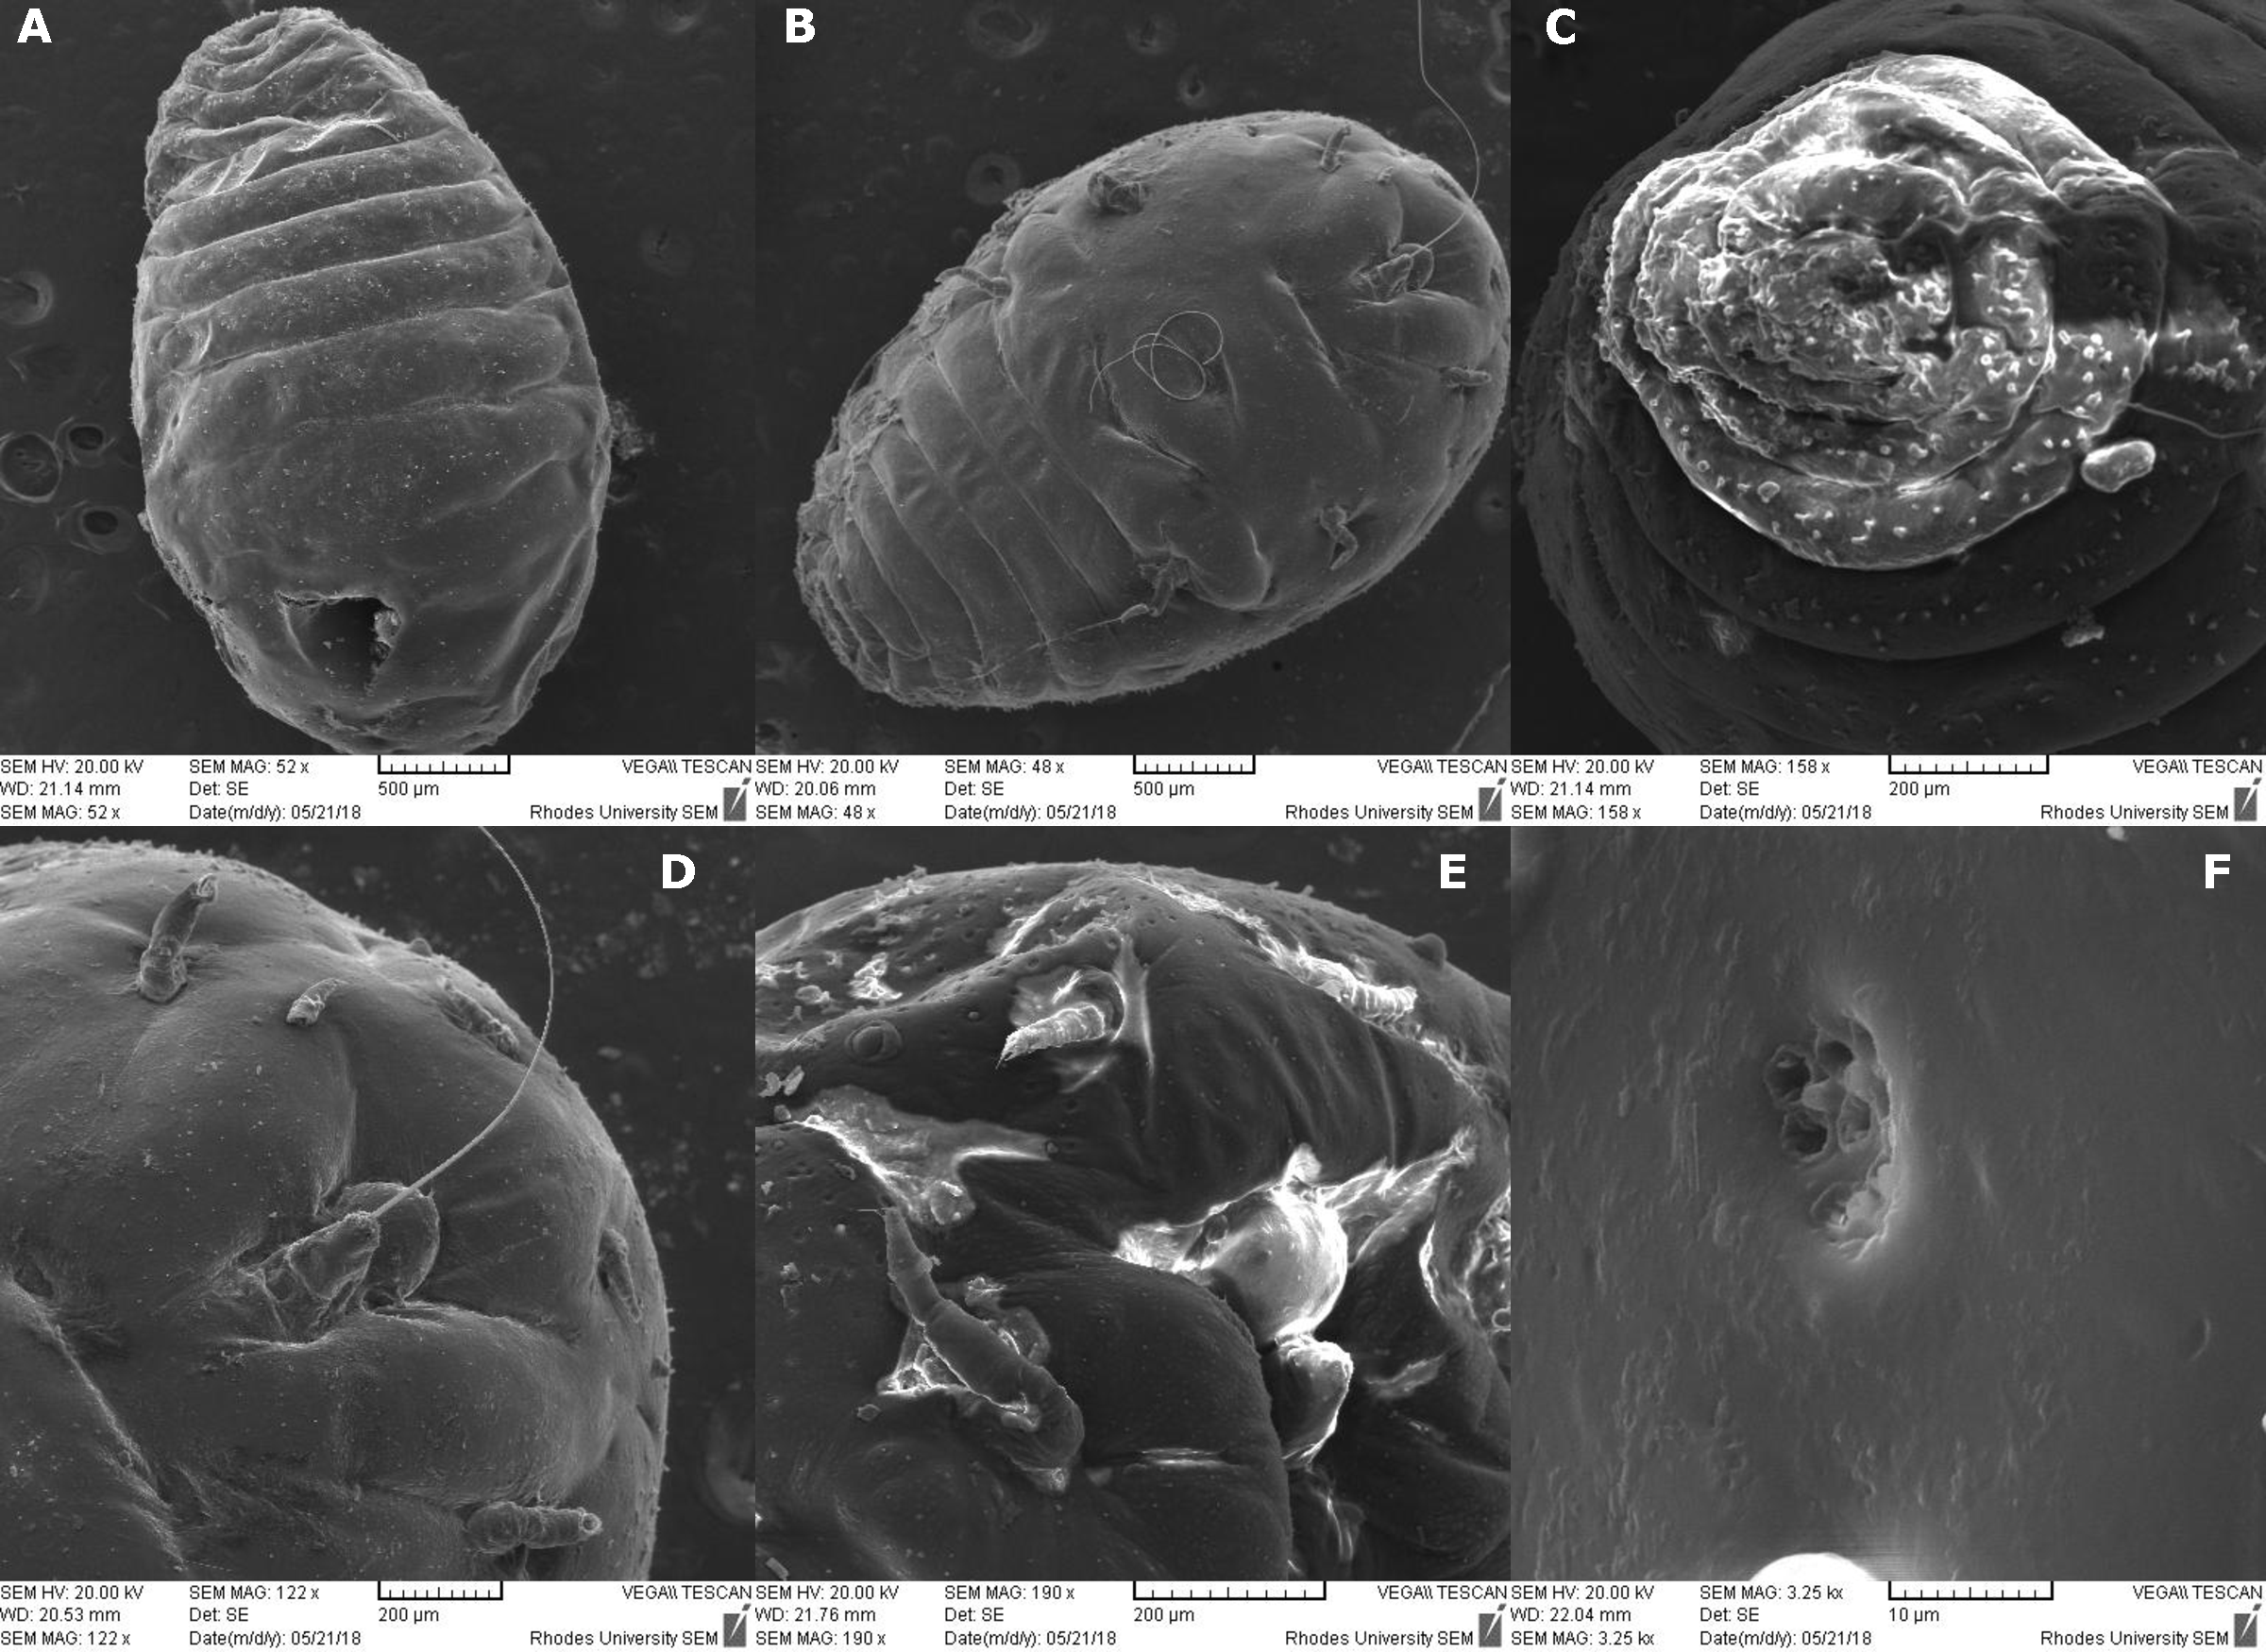
\includegraphics[scale =0.5]{Images/dactylopius_austrinus.pdf}
% 	\caption{} 
% 	\label{}
% \end{figure}
% \end{landscape}

% \begin{landscape}
% \begin{figure}[H]
% 	\centering
% 	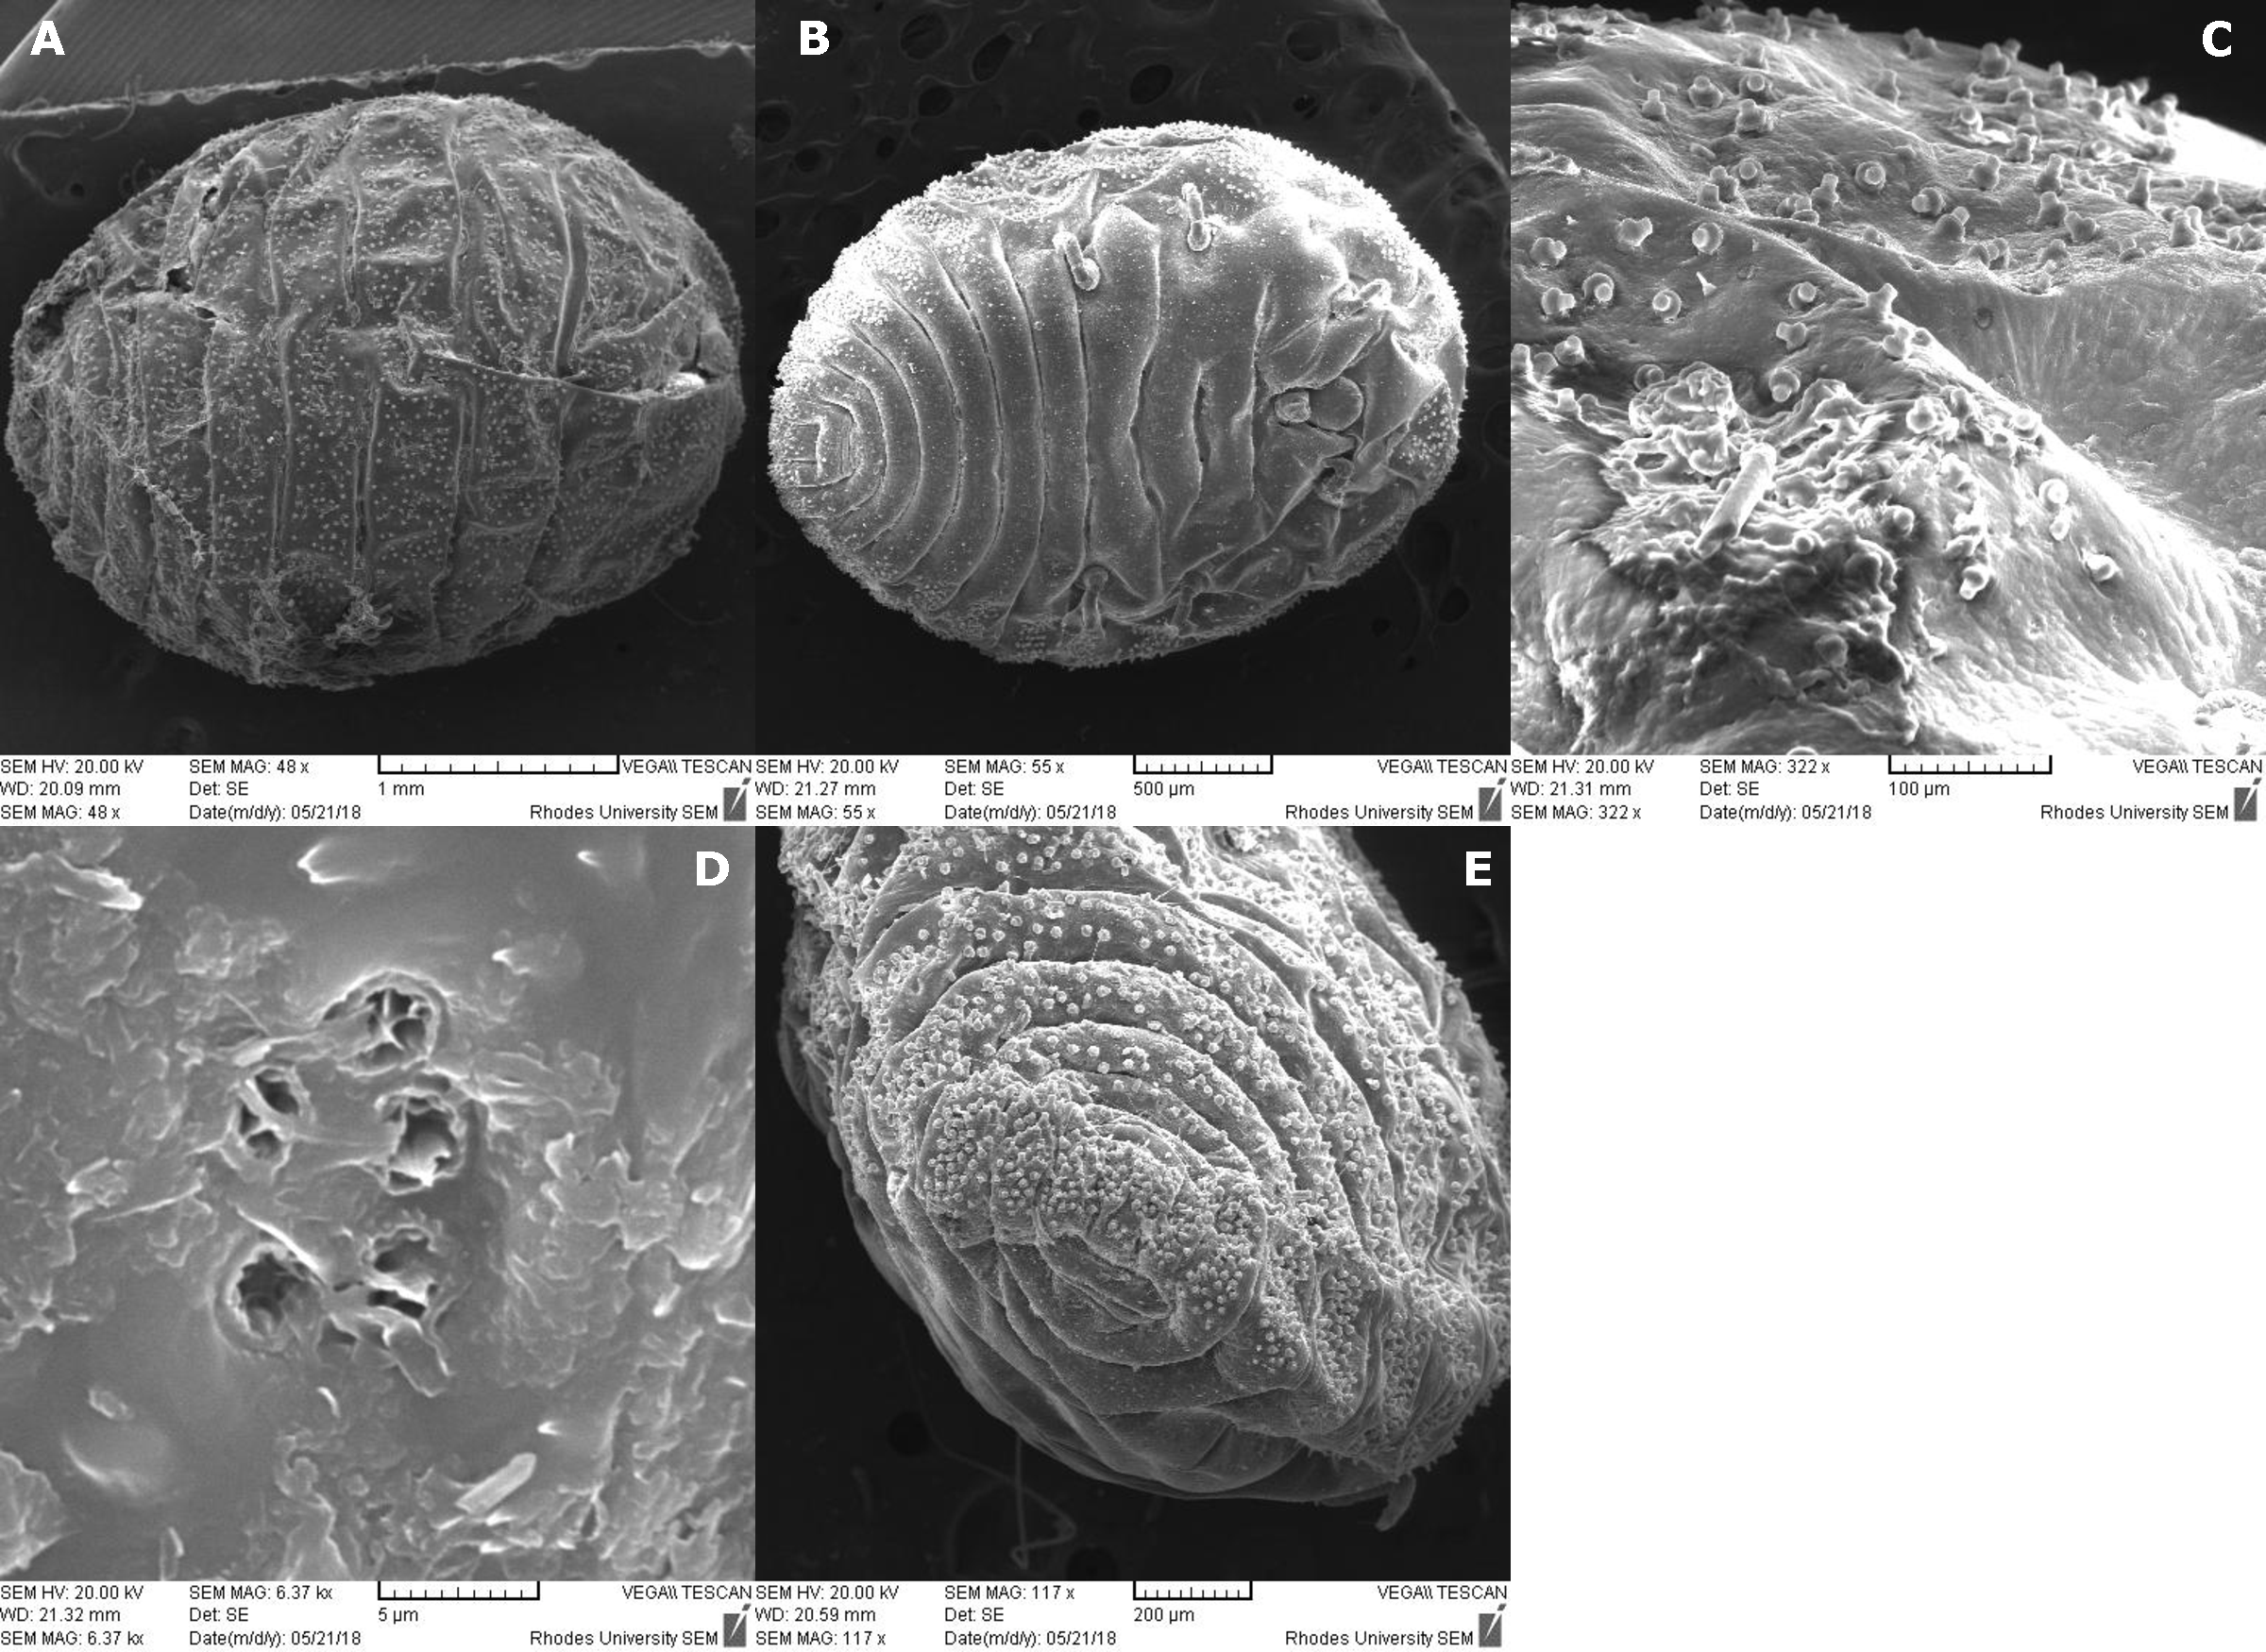
\includegraphics[scale =0.5]{Images/dactylopius_ceylonicus.pdf}
% 	\caption{} 
% 	\label{}
% \end{figure}
% \end{landscape}

% \begin{figure}[H]
% 	\centering
% 	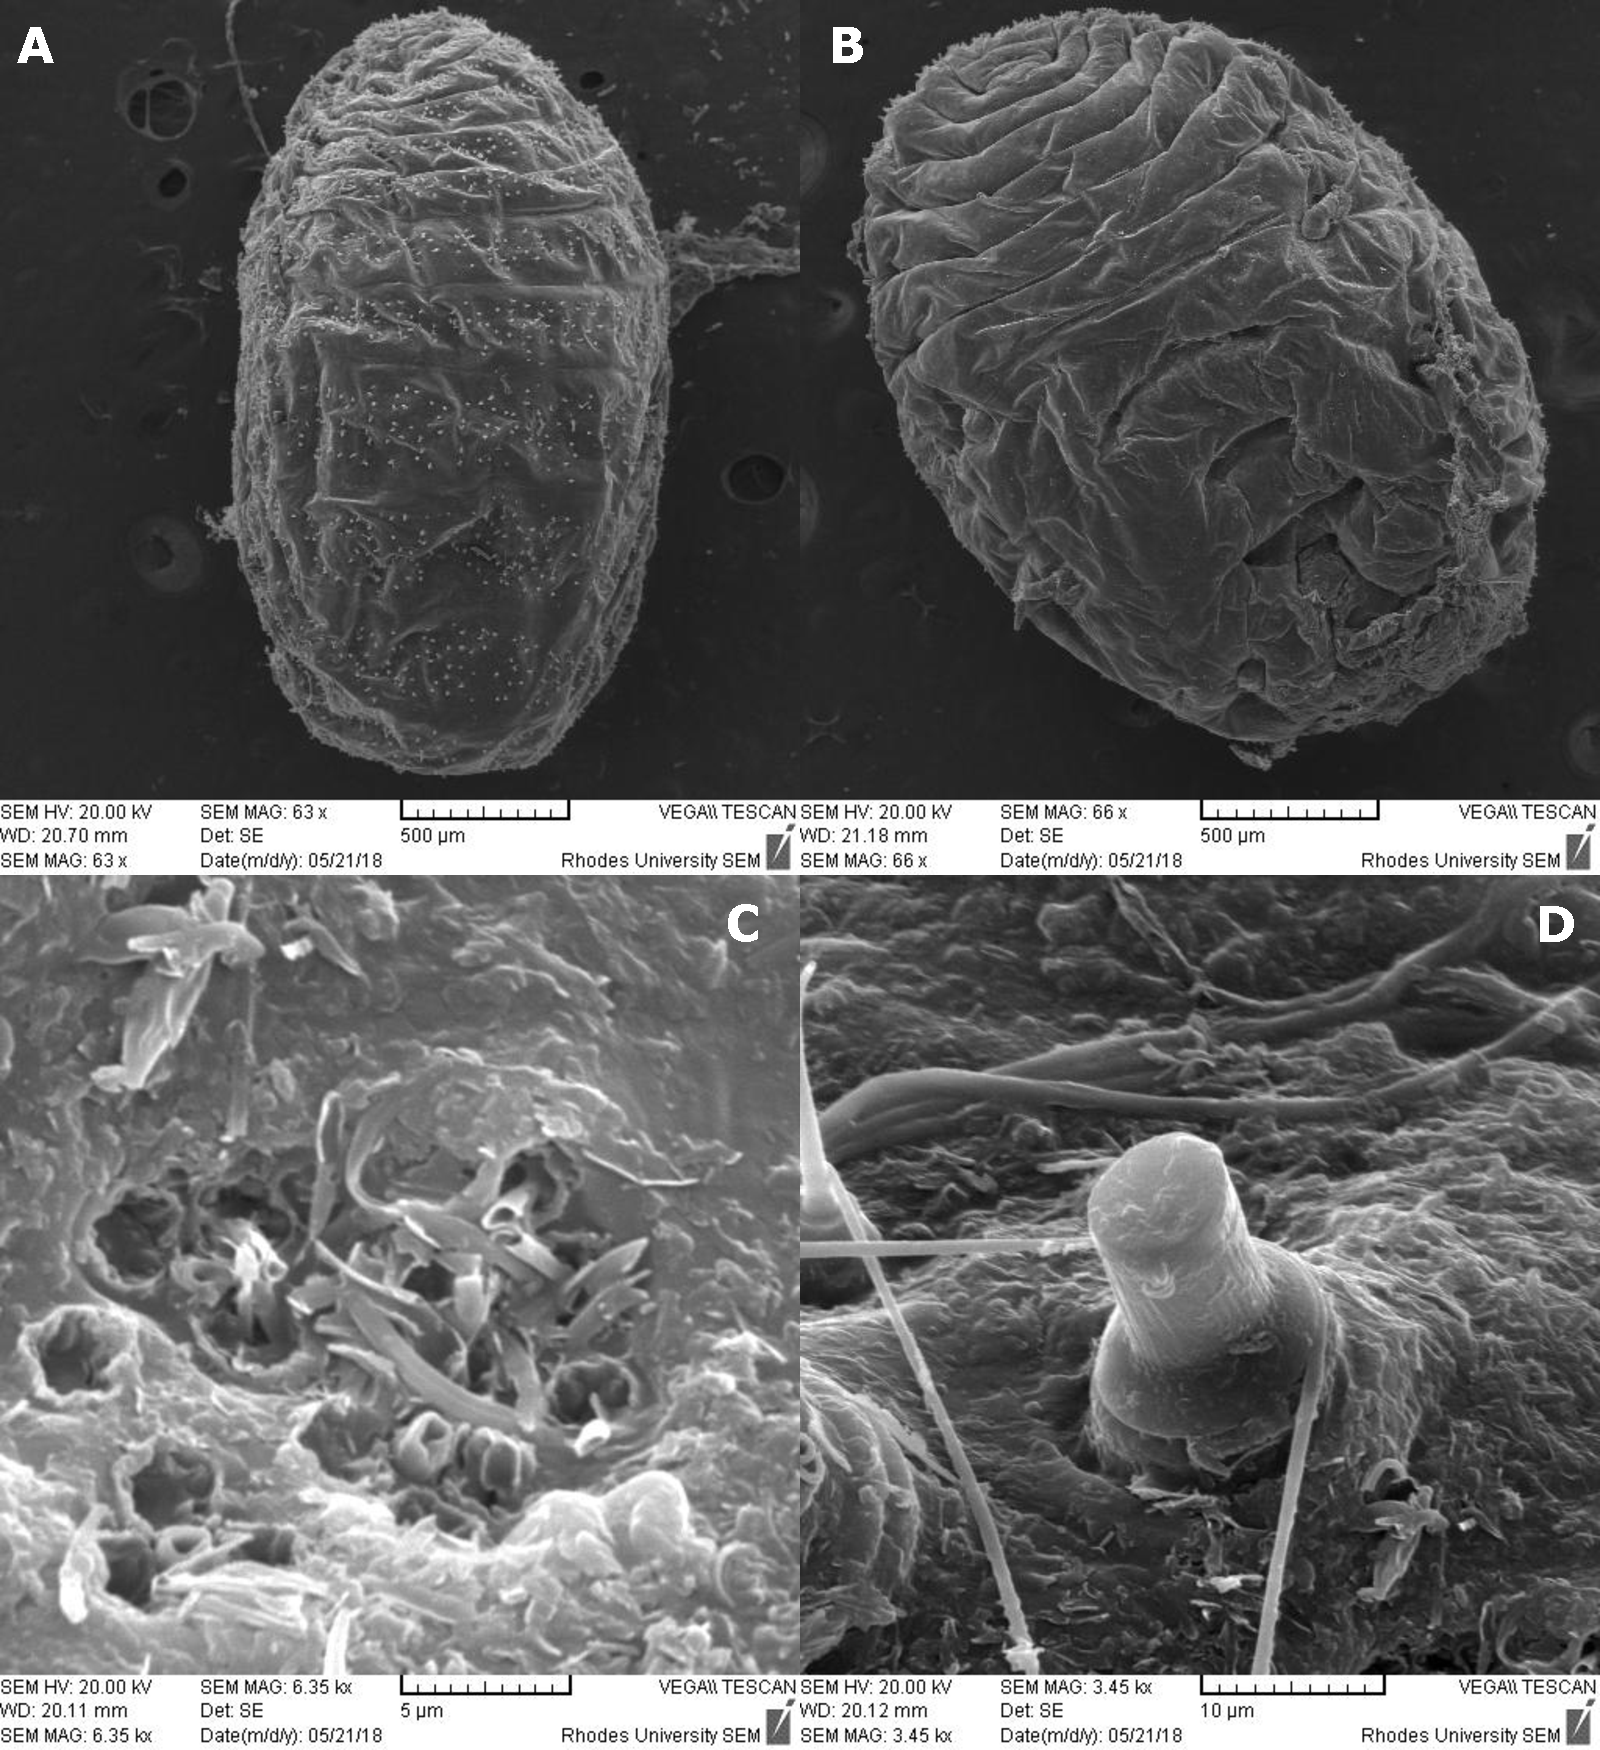
\includegraphics[scale =0.5]{Images/dactylopius_opuntiae_ficus.pdf}
% 	\caption{} 
% 	\label{}
% \end{figure}

% \begin{figure}[H]
% 	\centering
% 	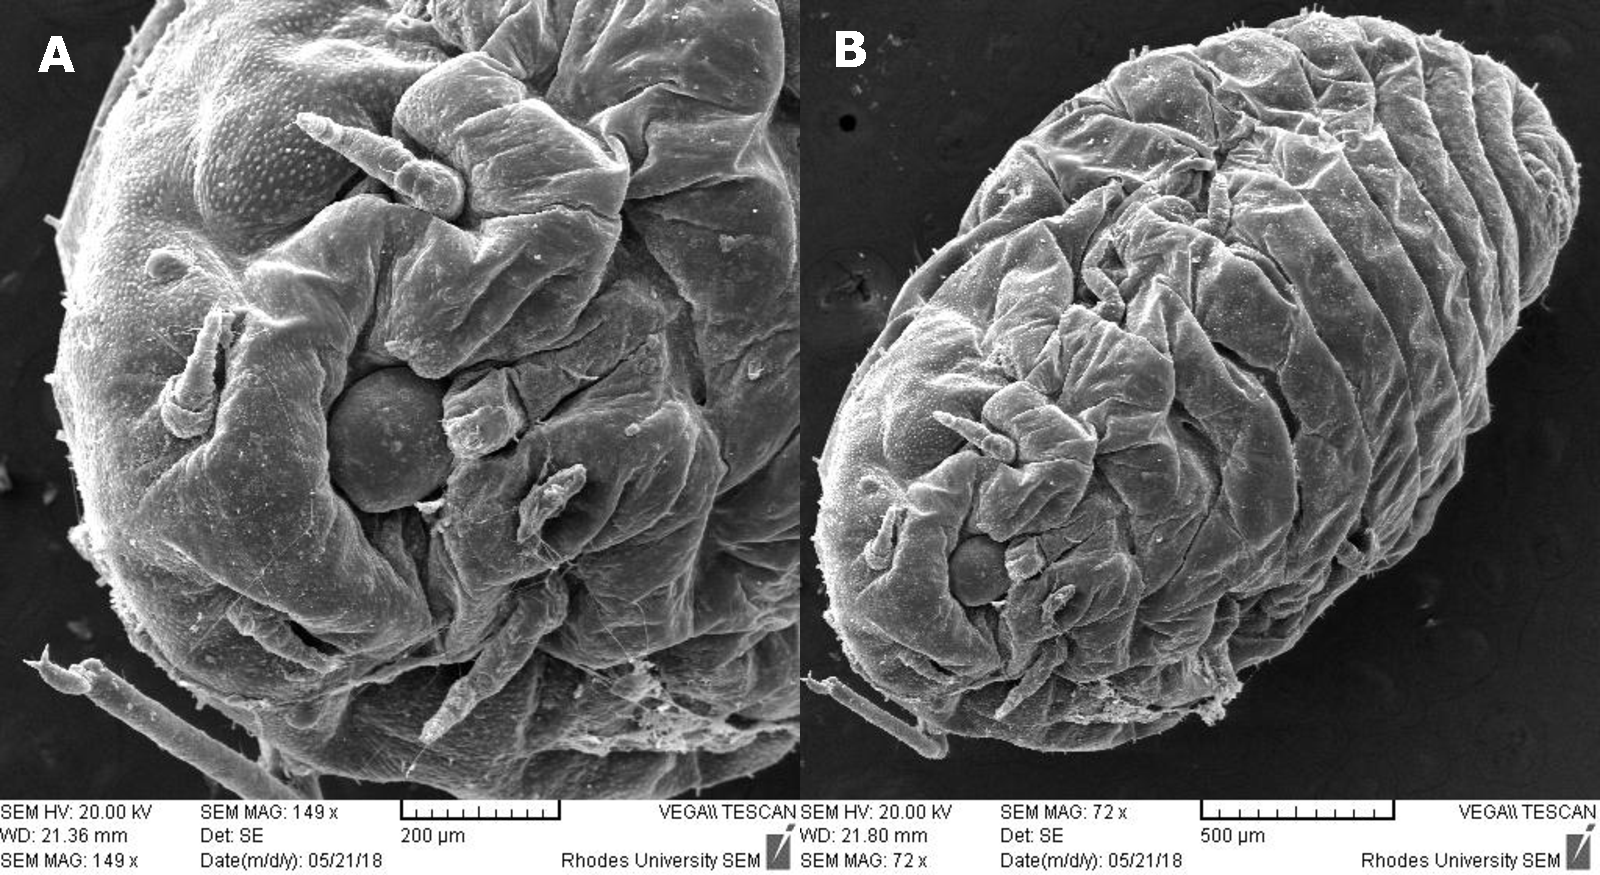
\includegraphics[scale =0.6]{Images/dactylopius_tomentosus_cholla.pdf}
% 	\caption{} 
% 	\label{}
% \end{figure}

% \begin{landscape}
% \begin{figure}[H]
% 	\centering
% 	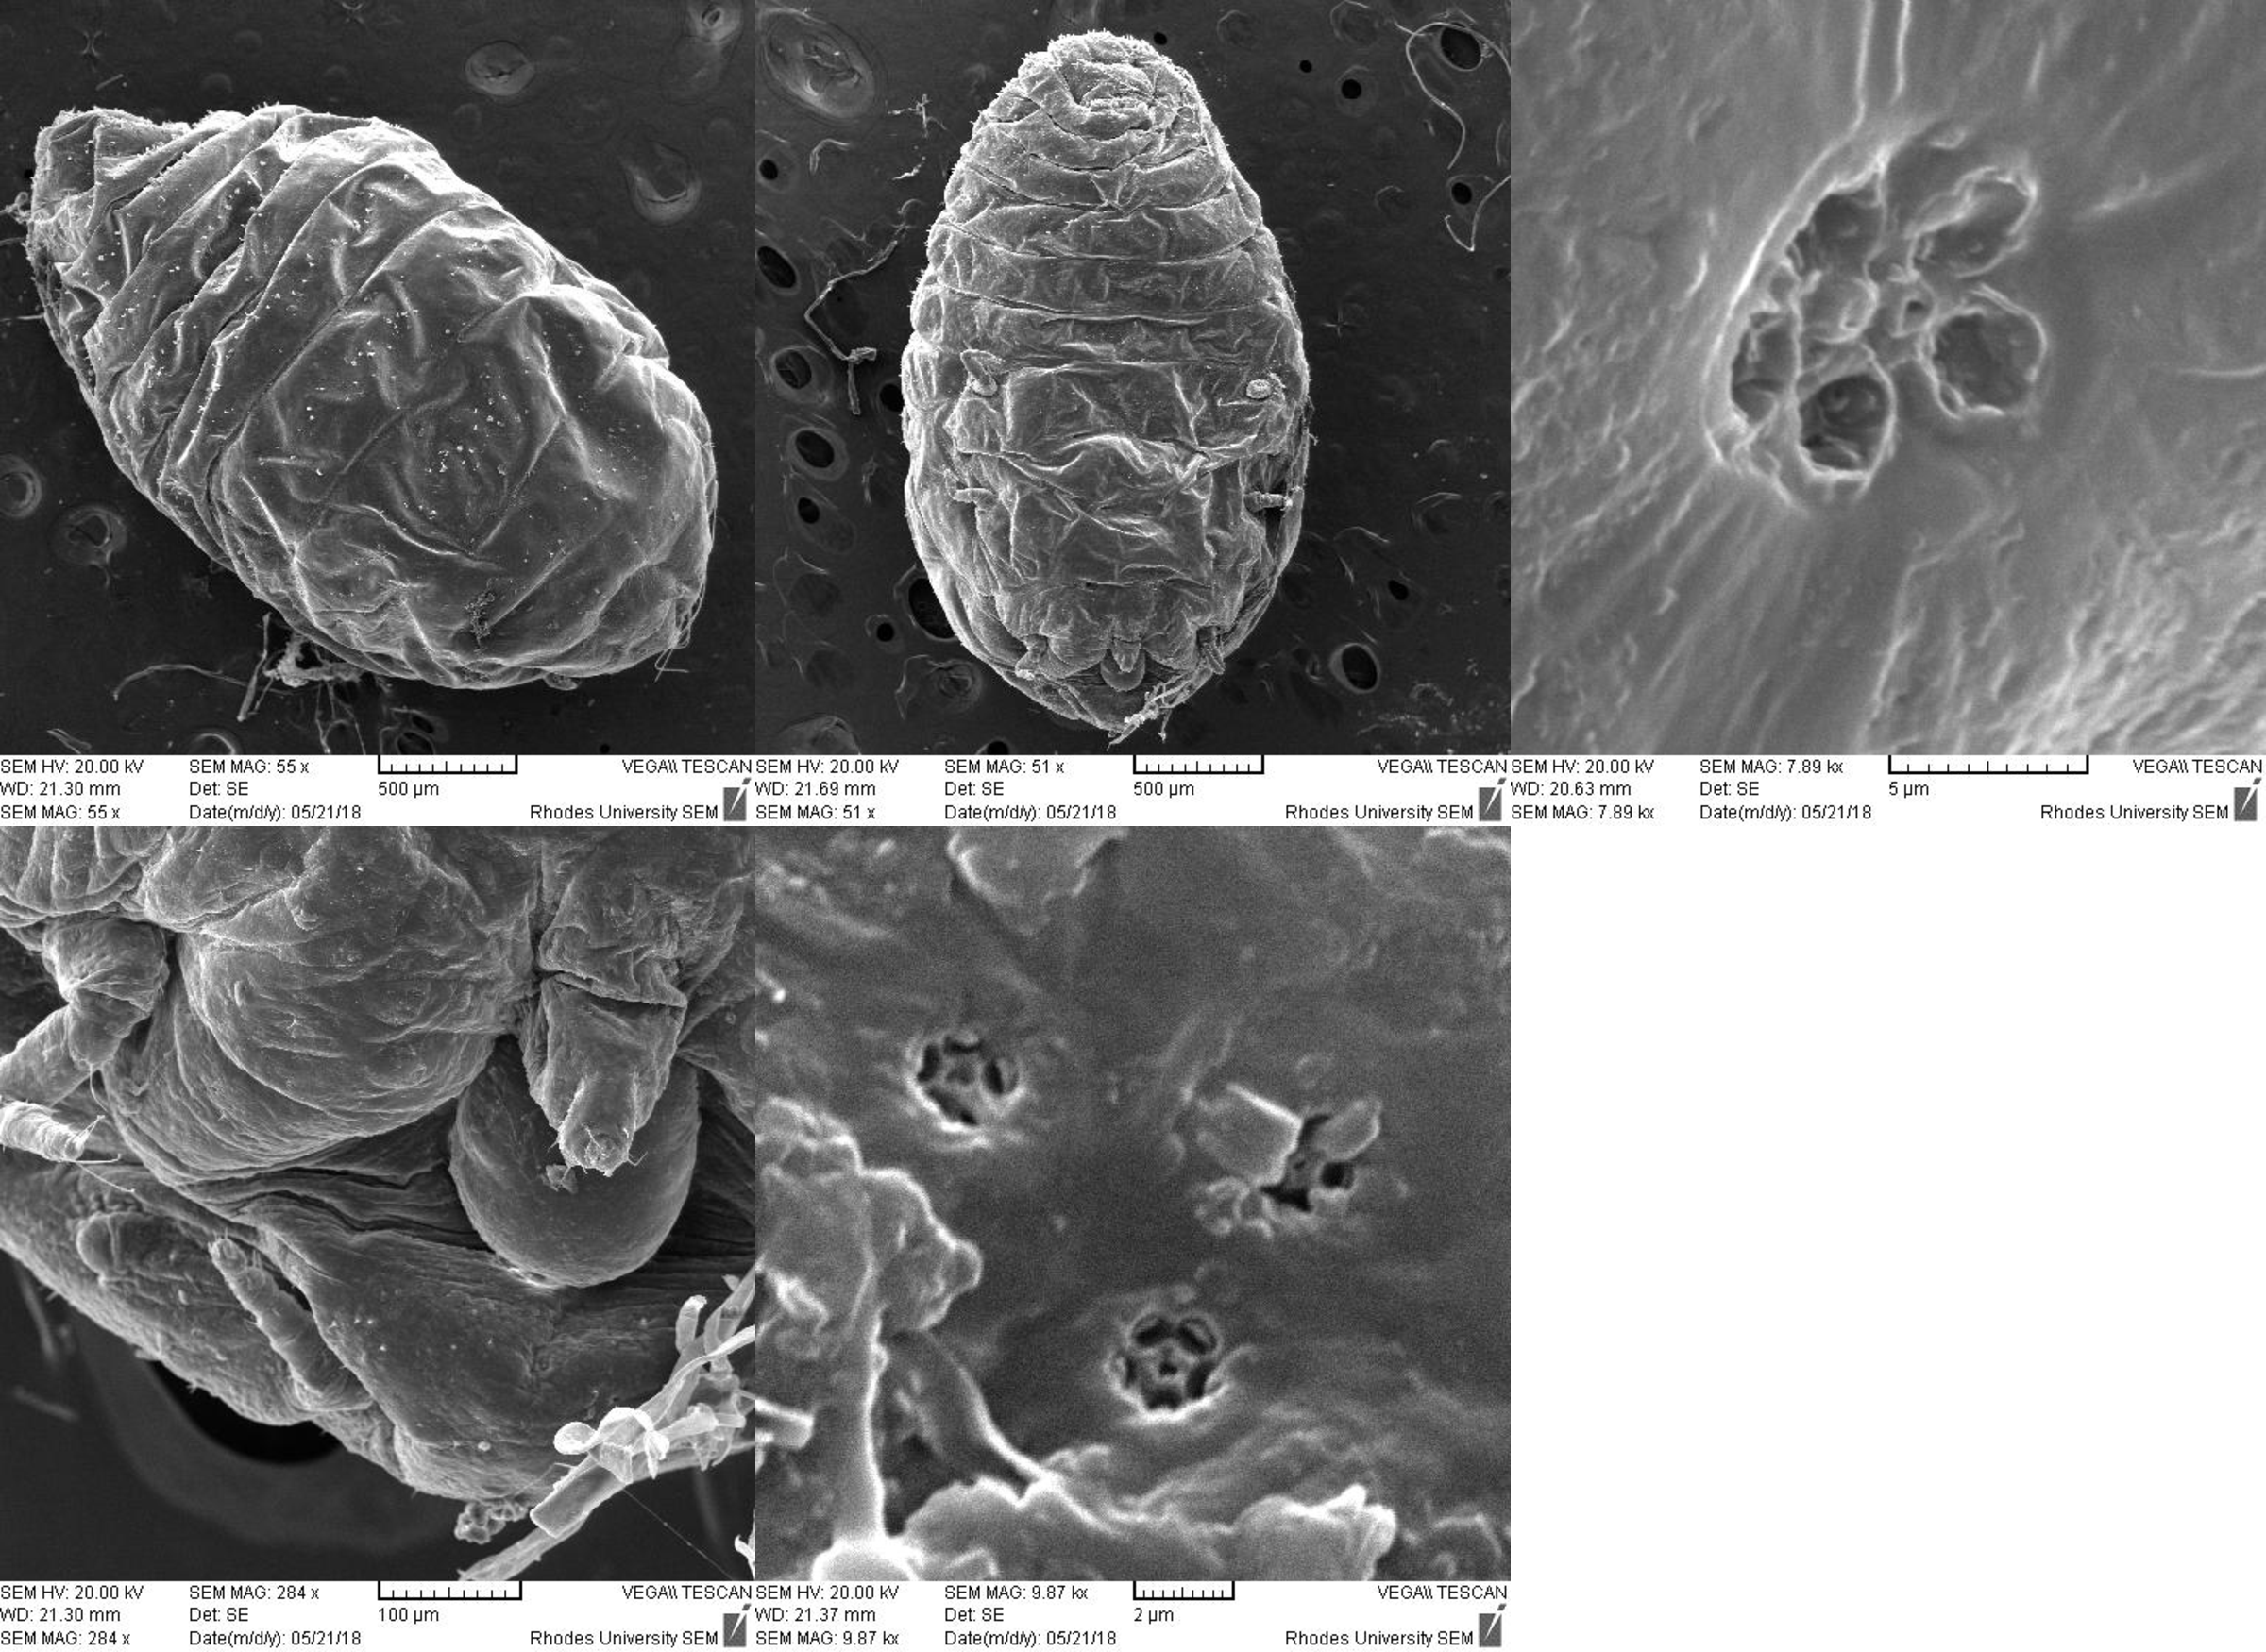
\includegraphics[scale =0.5]{Images/dactylopius_tomentosus_imbricata.pdf}
% 	\caption{} 
% 	\label{}
% \end{figure}
% \end{landscape}

\section{R Scripts}
\label{appendix:rScripts}

\subsection{Barcode testing using SPIDER}
\label{appendix:RCODE,SPIDER}
% \textbf{R code for the basic barcode testing algorithms in the Spider package, adapted from the tutorial by \citet{Brown2012Spider:Barcoding}} \\

\begin{lstlisting}[language=R]
# Read in a .fas file
setwd("file_location")
getwd()
input = "file_name.fas"
seqs = read.dna(input, format = 'fas')
dist = dist.dna(seqs, pairwise.deletion = TRUE)
# Nearest neighbour:
sppNames = dimnames(seqs)
table(nearNeighbour(dist, sppNames))
# Threshold Identification:
table(threshID(dist, sppNames, threshold = 0.01))
# Meier's Best Close Match:
table(bestCloseMatch(dist, sppNames, threshold = 0.01))
# Optimising the threshold value from the default of 0.01:
threshVal = seq(0.001,0.02, by = 0.001)
sens = lapply(threshVal, function(x) threshOpt(dist, sppNames, thresh = x))
sensMat = do.call(rbind, sens)
barplot(t(sensMat)[4:5,], names.arg=paste((sensMat[,1]*100), "%"))
# Graphically displaying the barcoding gap:
inter = nonConDist(dist, sppNames) *100
intra = maxInDist(dist, sppNames) *100
bnd = cbind(data.frame(inter, intra))
ord = bnd[order(bnd$inter),]
plot(ord$inter, type="n", ylab="Percent K2P distance", xlab="Individual")
segCol = rep("gray50", length(ord$inter))
segCol[ord$inter-ord$intra < 0] = "red" 
segments(x0=1:length(ord$inter), y0=ord$inter, y1=ord$intra, col=segCol, lwd=6)
\end{lstlisting}

\subsection{Jaccard's transformation}
% Jaccard's transformation was applied in R using the `dist' function with the `binary' method using the following code: \newline
\label{appendix:RCODE,Jaccard}
\begin{lstlisting}[language=R]
binarymat <-read.csv("file_name.csv", header = T, sep = ",", dec = ".")
# removes the first two columns, which contain sample names and grouping information
binarymat2 = binarymat[,c(-1,-2)] 
# assign sample names as row names 
row.names(binarymat2) = binarymat[,1] 
# shortens the names to 10 characters
newnames =substring(row.names(binarymat2), 0, 10) 
row.names(binarymat2) = newnames
# replaces ? with NA, as NA's are ignored.
binarymat2[binarymat2=="?"] <- NA 
# converts the matrix to a data frame 
binarymat2 = as.data.frame(binarymat2) 
# creates a distance matrix
d = dist((binarymat2), method = "binary", diag = TRUE, upper = T) 
d = as.data.frame(as.matrix(d))
d2 =  as.dist(d)

\end{lstlisting}

\subsection{UPGMA clustering tree}
\label{appendix:RCODE,upgma}
\begin{lstlisting}[language=R]
library(pvclust)
# 'average' refers to the UPGMA method. 
# binarymat2 is transformed such that the data is organised by column.
result <- pvclust(t(binarymat2), method.dist = "binary", method.hclust="average", nboot=1000) 
p = plot(result, cex = 0.6, print.num = F, print.pv = T, cex.pv = 0.6)

\end{lstlisting}

\subsection{Non-metric MDS plot}
\label{appendix:RCODE, nmds}
\begin{lstlisting}[language=R]
# k is the number of dimensions
# d2 is the distance matrix obtained for the data using the `binary' method
fit <- isoMDS(d2, k=2) 
# view the stress value
fit$stress 
mds_plot = isoMDS(d2,k=2)
eqscplot(mds_plot$points, col = c("red", "dodgerblue3", "forestgreen", "orange")[binarymat$Group], pch = c(15, 16, 17,18)[binmat$Group])
# the number of colours and pch types selected will depend on the number of groups (binarymat$Group) inputted
scree.plot = function(d, k) {
stresses=isoMDS(d, k=k)$stress
  for(i in rev(seq(k-1)))  
  stresses=append(stresses,isoMDS(d, k=i)$stress)
  plot(seq(k),rev(stresses), type="b", xaxp=c(1,k, k-1), ylab="Stress", xlab="Number of dimensions")
}
# plot stress values for six dimensions
scree.plot(d2, k=6) 
shep<-Shepard(d2, mds_plot$points, p=2)
plot(shep, pch=".", main = "K = 2")
# R squared value
summary(lm(shep$y~shep$x)) 
# line of best fit through the points
abline(lm(shep$y~shep$x), col = "red", lty = 2) 
\end{lstlisting}

\subsection{Three dimensional non-metric MDS plot}
Although not included in the results, three dimensional nMDS (Non-metric Multidimensional Scaling) scatter plots were created in R using the plot3D package \citep{Soetaert}. The following following code was implemented: \newline

\begin{lstlisting}[language=R]
# nMDS with three dimensions
fit <- isoMDS(d2, k=3) 
x <- fit$points[,1]
y <- fit$points[,2]
z <- fit$points[,3]
library(plot3D)
# points are coloured by group, which was column 2 in the original binarymat matrix
scatter3D(x,y,z, phi = 25,  type = "h", 
pch = 19, cex = 1.5, bty = "b", colvar = as.integer(binarymat$Group), col = c("blue", "red"), colkey = list(side = 2, length = 0.5))
# an optional addition to add sample names above points in the scatter plot
text3D(x, y, z, labels = rownames(binarymat2), add = TRUE, colkey = FALSE, cex = 0.7) 
\end{lstlisting}

\subsection{ANOSIM and PERMANOVA}
\label{appendix:RCODE,anosim,permanova}
\begin{lstlisting}[language=R]
# ANOSIM:
anosim(d2, binarymat$Group, permutations = 999, distance = "jaccard")
# PERMANOVA:
library(vegan)
adonis(d2~binarymat$Group)
library(RVAideMemoire)
pairwise.perm.manova(d2, binarymat$Group)
\end{lstlisting}


\begin{landscape}
\section{Shiny Applications}
\begin{figure}[H]
	\centering
	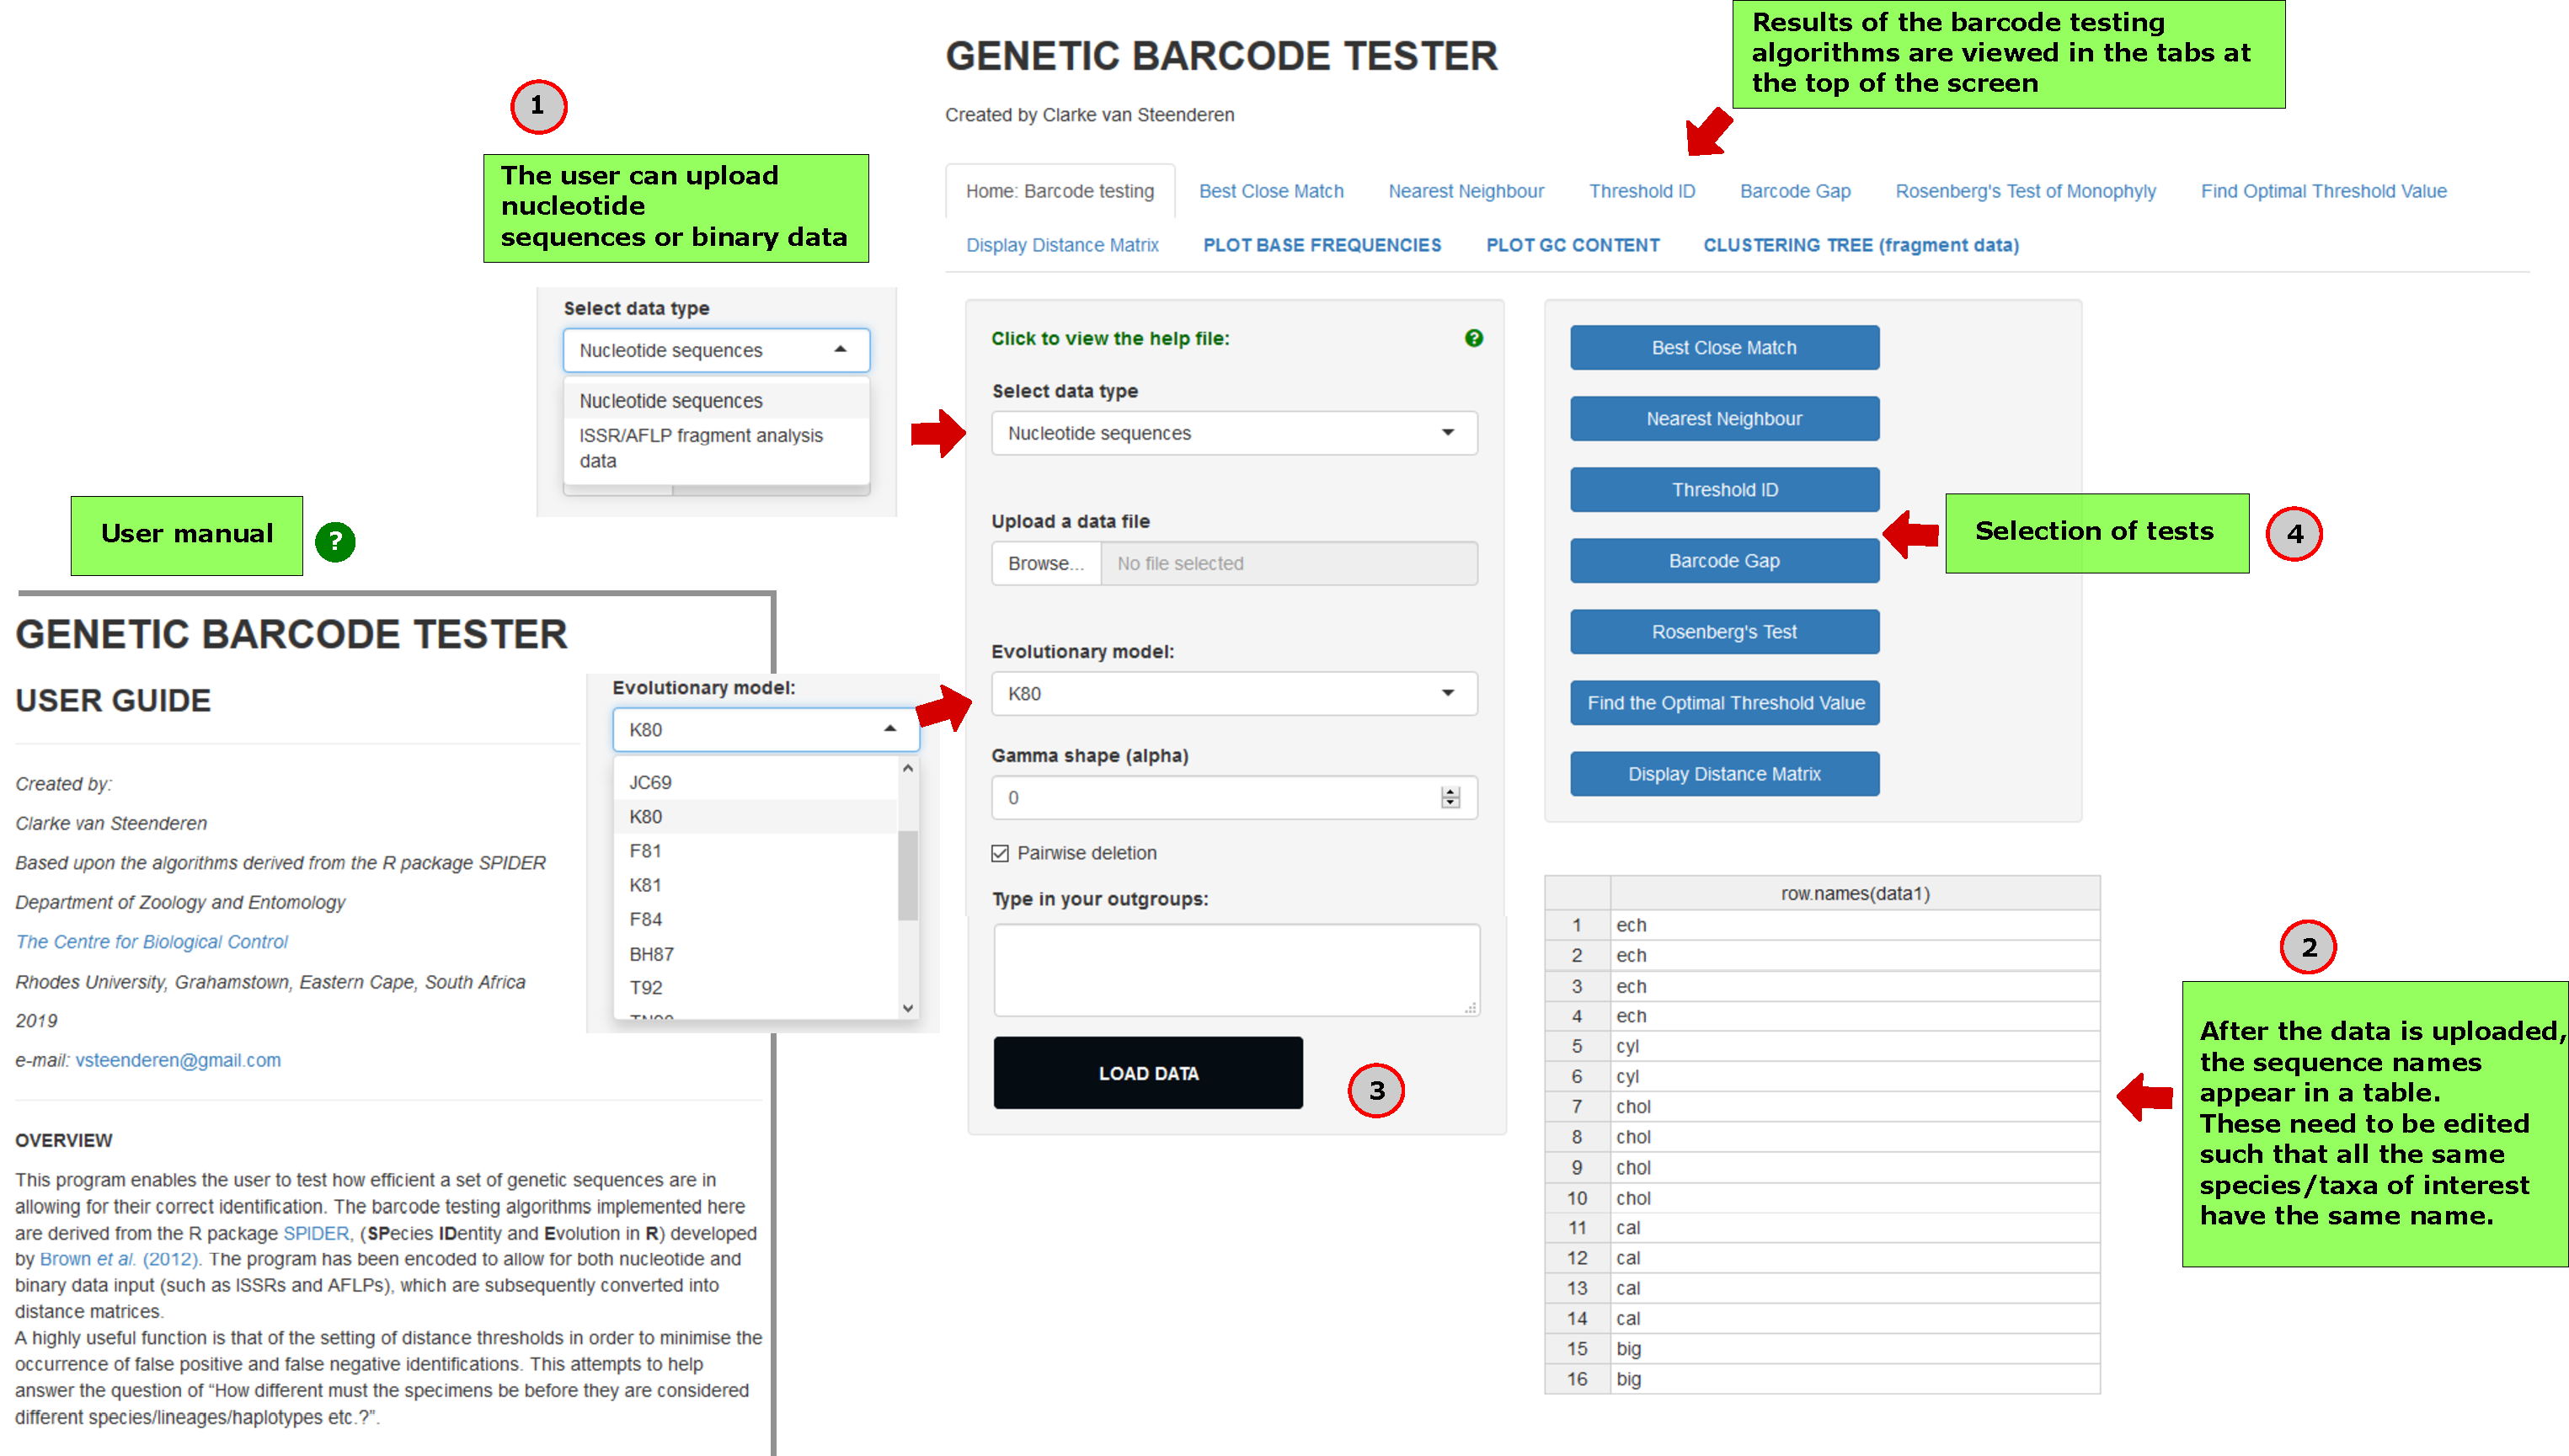
\includegraphics[scale = 0.42]{Images/barcode_tester_gui.pdf}
    \newline
	\caption{Genetic barcode tester GUI showing the components of the application. Numbers in circles indicate the order in which data is uploaded and processed.}. 
	\label{fig:barcodeTesterGUI}
\end{figure}
\end{landscape}

\begin{landscape}
\begin{figure}[H]
	\centering
	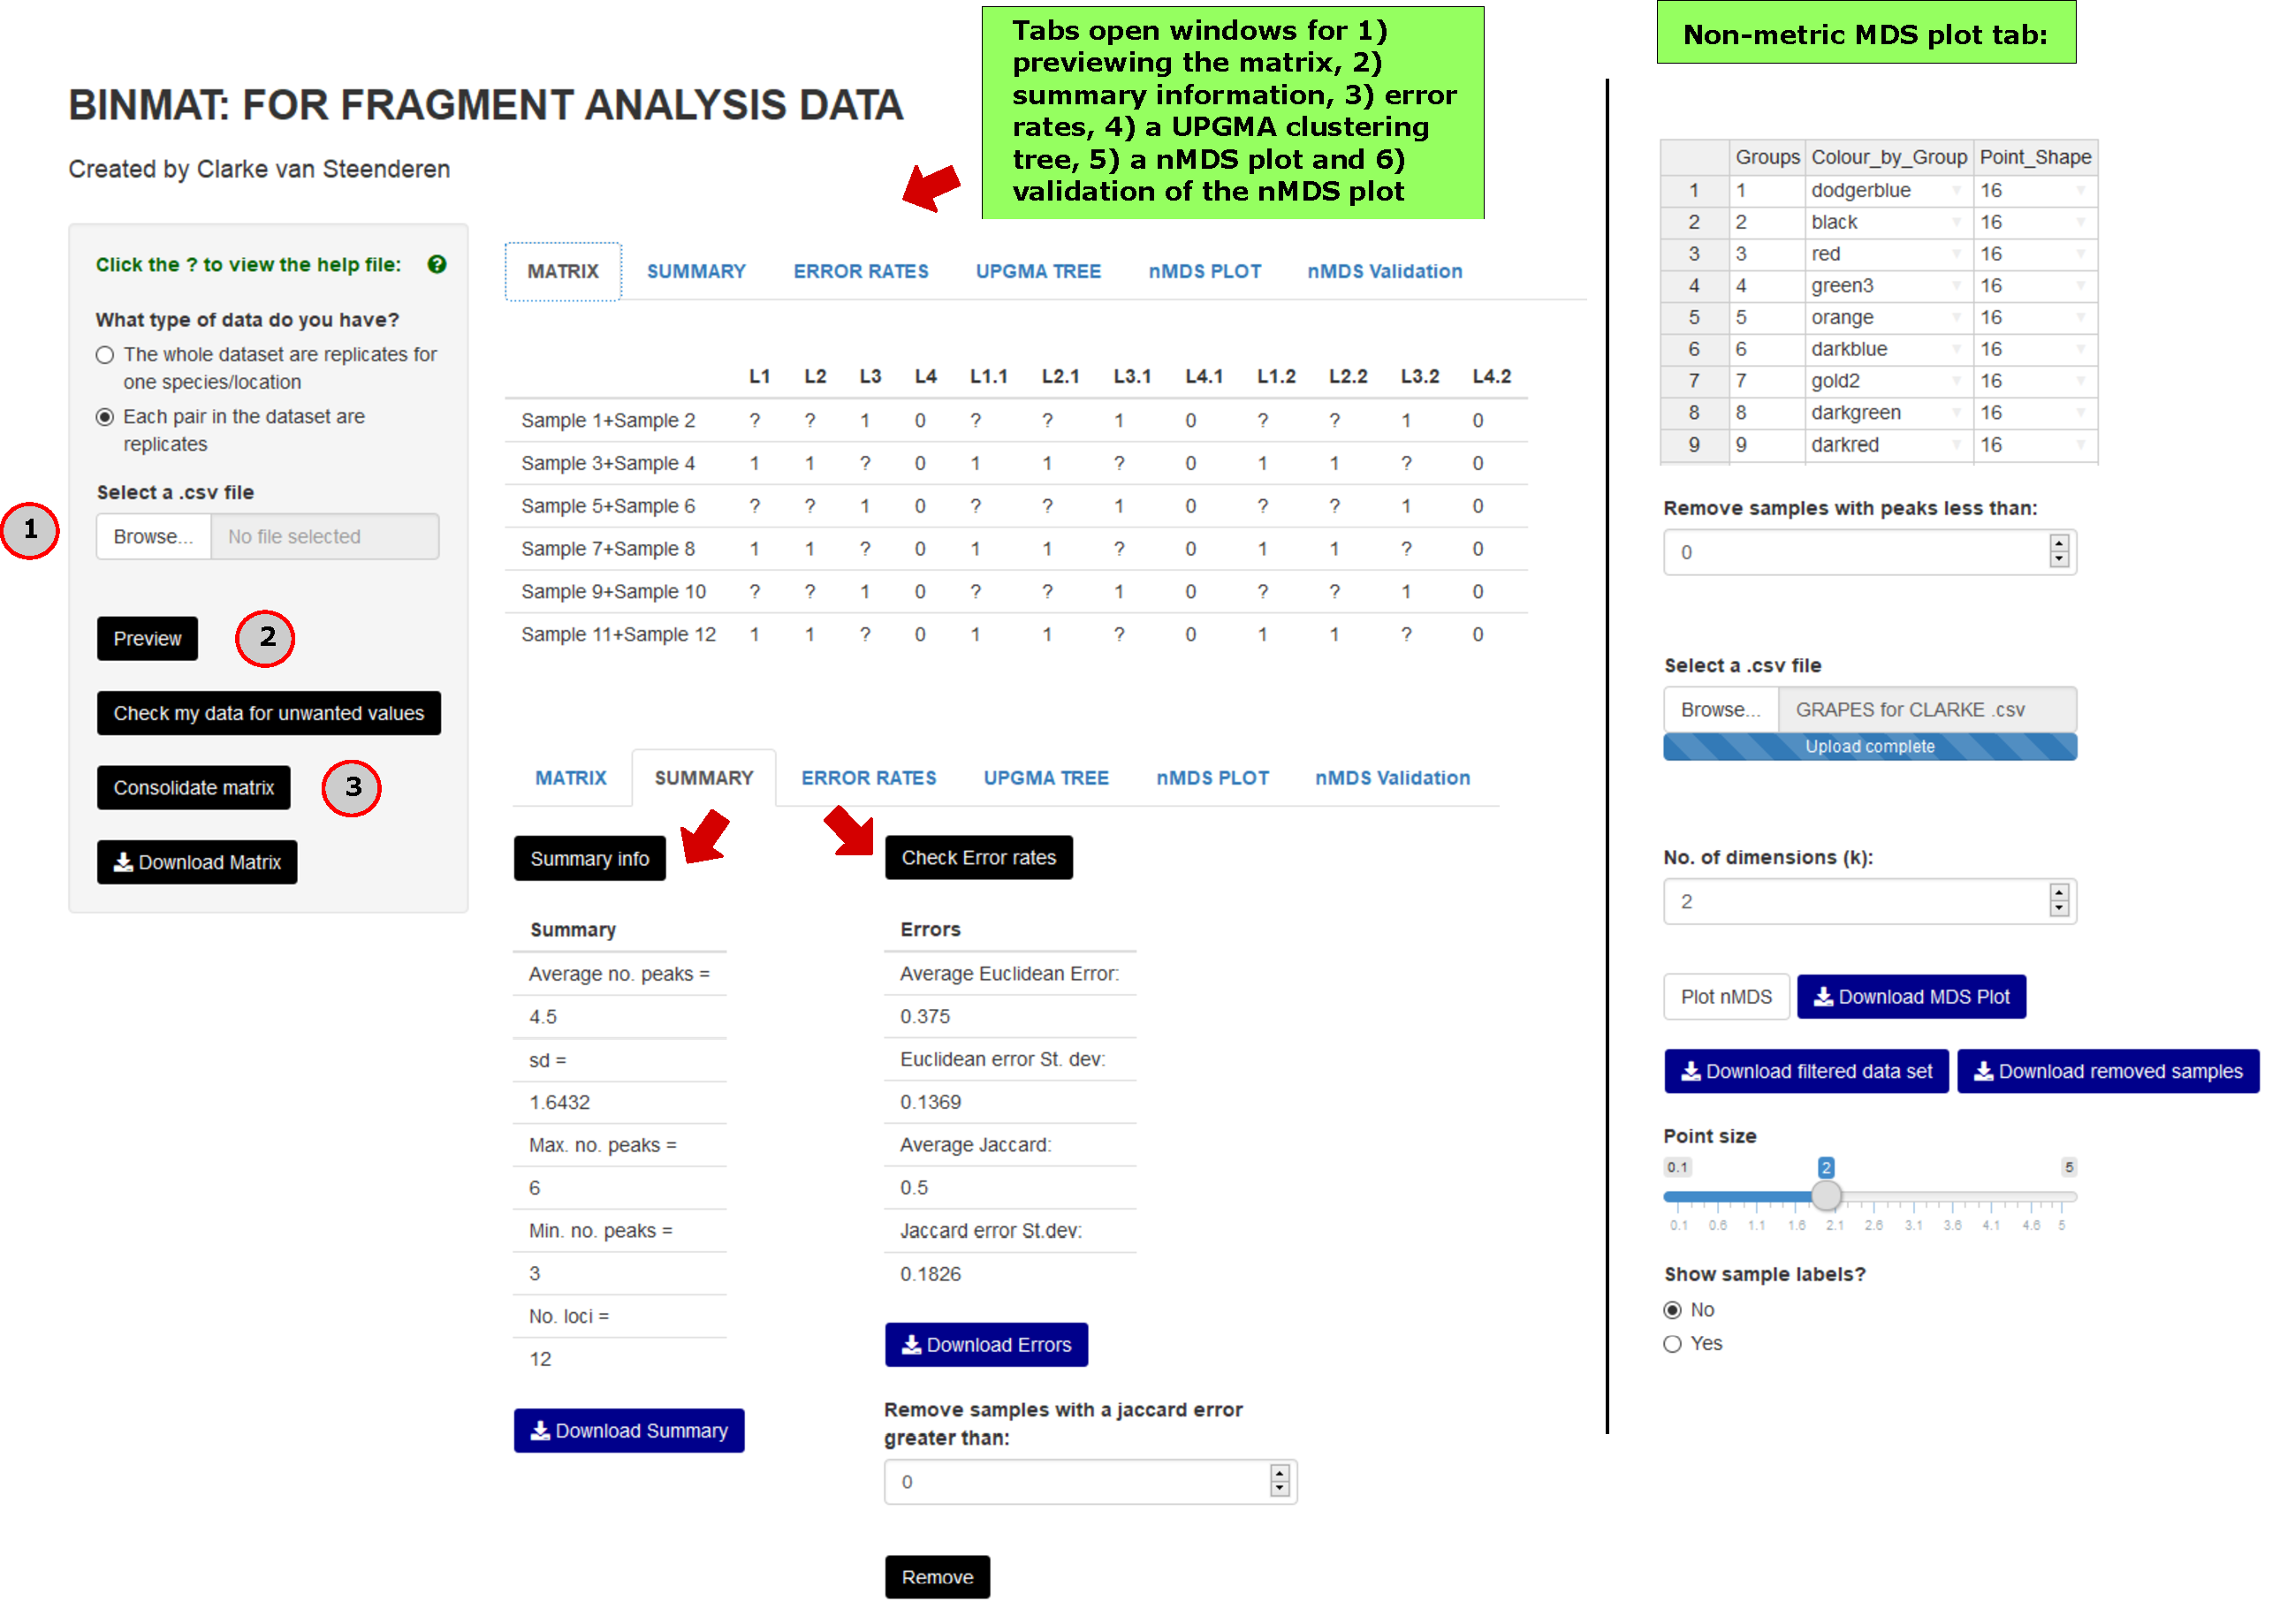
\includegraphics[scale = 0.45]{Images/binmat_gui.pdf}
    \newline
	\caption{Binary matrix processing application (`BINMAT'), where the user uploads a .csv file containing binary data replicates in order to consolidate them. Summary statistics, error rates and the construction of a UPGMA clustering tree are also available. Non-metric MDS plots can be created by uploading a consolidated binary matrix, where filtering of samples with a low peak count can be applied.} 
	\label{fig:binmatGUI}
\end{figure}
\end{landscape}

\subsection{Dacty-ID}

When uploading this application to the Shiny server, the following command was required in R in order to set the repositories to access packages within Bioconductor (namely the DECIPHER package by \citet{wright2016using}): \\ \\
\noindent
\texttt{
setRepositories() \\
} \\
\noindent This produced the output on the console: \\ \\
\texttt{
\noindent 1: + CRAN \\
2:   BioC software \\
3:   BioC annotation \\
4:   BioC experiment \\
5:   CRAN (extras) \\
6:   Omegahat \\
7:   R-Forge \\
8:   rforge.net \\
Enter one or more numbers separated by spaces, or an empty line to cancel \\
1: } \\

\noindent Options 2, 3, and 4 were entered to include all the BioC-related dependencies.

\begin{landscape}
\begin{figure}[H]
	\centering
	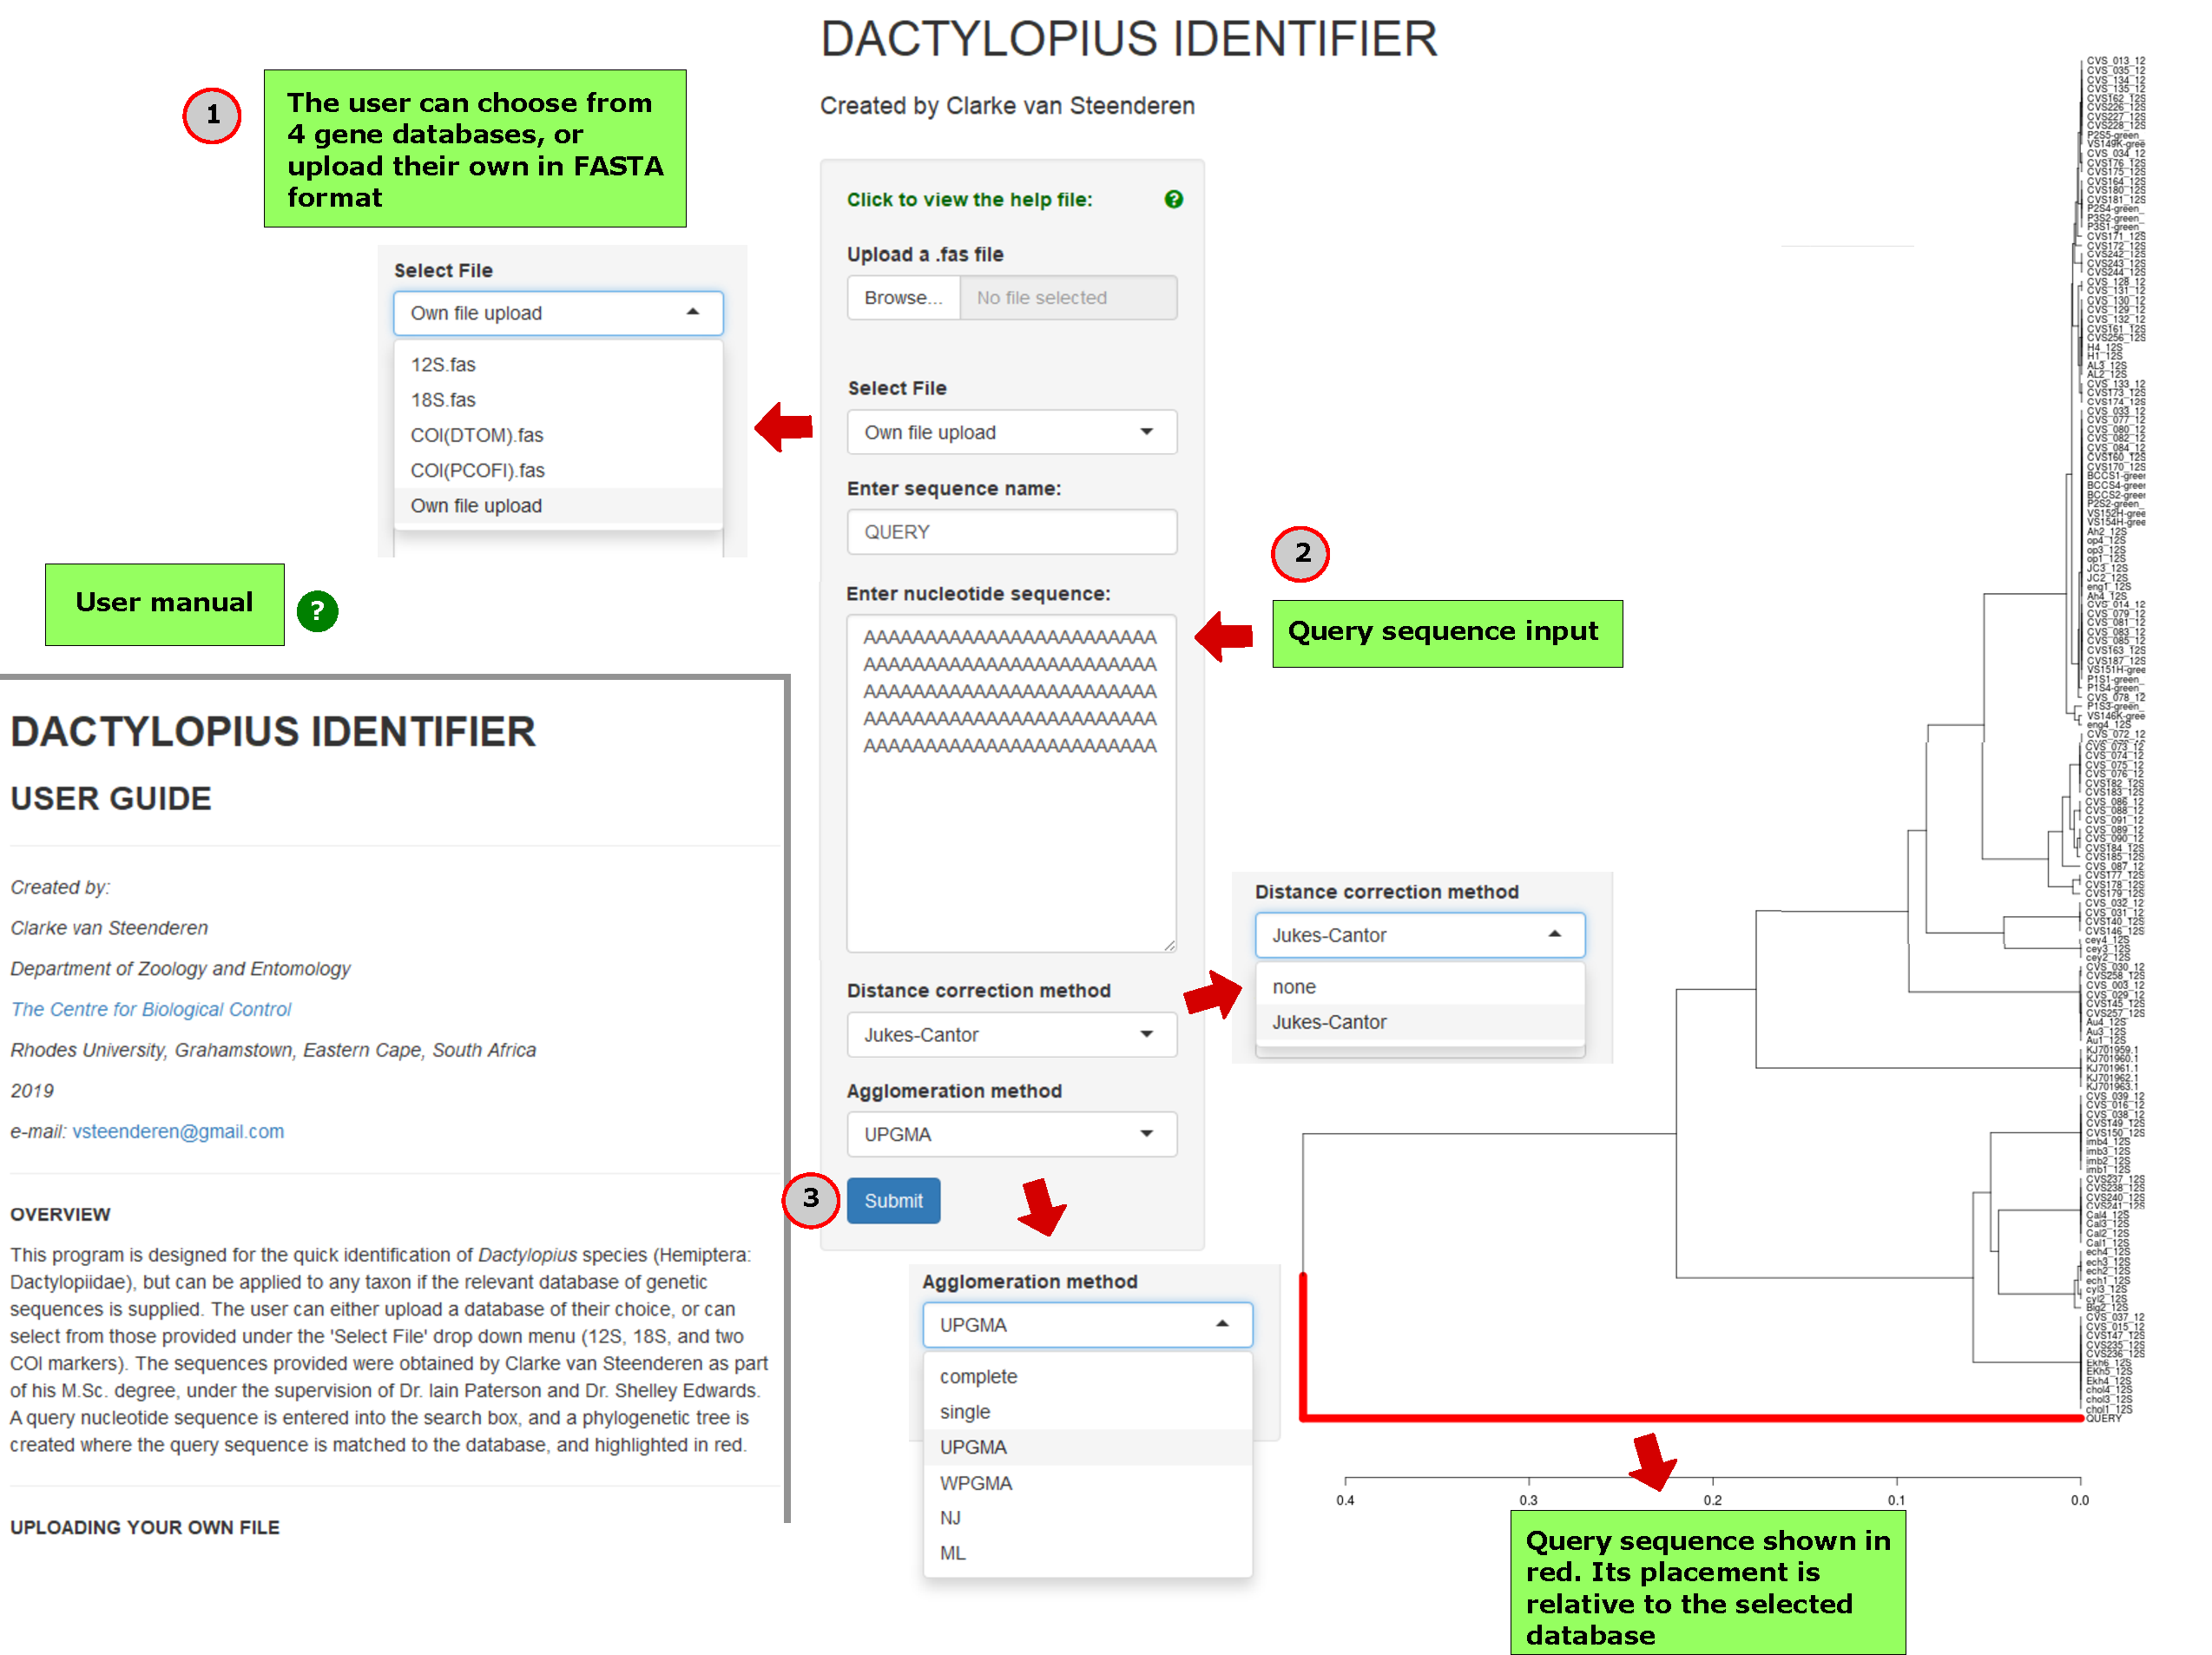
\includegraphics[scale = 0.4]{Images/dactylopius_identifier_GUI.pdf}
	\caption{Identification GUI application, where the user can test the identity of a query sequence against a preselected genetic database. A phylogenetic tree is displayed on the screen, with the position of the query sequence highlighted in red.}
	\label{fig:identifier_GUI}
\end{figure}
\end{landscape}

\section{MRBAYES Nexus files}
\label{appendix:bayesblocks}

\subsection{12S}
\fbox{\parbox{\textwidth}{%
{\parindent0pt %

\#NEXUS \\
{[12S aligned sequences]} \\

begin data; \\
dimensions ntax=152 nchar=779; \\
format interleave datatype=DNA missing=N gap=-; \\

matrix \\
ALIGNED 12S SEQUENCES \\
; \\
end; \\

begin mrbayes; \\
	set autoclose=yes nowarn=yes; \\
	lset nst=6 rates=gamma ngammacat = 4 code=universal; \\
	outgroup HQ893819.1; \\
	prset revmatpr = dirichlet(6.0485, 8.2345, 15.0465, 0.0004, 42.1397, 1.0000) \\
	statefreqpr = dirichlet(0.3923, 0.1404, 0.1629, 0.3044) \\
	shapepr = fixed(0.8960); \\
	mcmc Ngen=50000000 printfreq=1000 samplefreq=1000 Nchains=4 savebrlens=yes starttree=random; \\
	sumt burnin = 1250; \\
	sump burnin = 1250; 
  
end; \\

}%
}} %

\subsection{18S}

\fbox{\parbox{\textwidth}{%
{\parindent0pt %

\#NEXUS \\
{[18S aligned sequences]} \\

begin data; \\
dimensions ntax=153 nchar=630; \\
format interleave datatype=DNA missing=N gap=-; \\

matrix \\
ALIGNED 18S SEQUENCES \\
; \\
end; \\

begin mrbayes; \\
set autoclose=yes nowarn=yes; \\
	lset nst=6 rates=propinv ngammacat = 4 code=universal; \\
	outgroup KY9276001; \\
	prset revmatpr = dirichlet(0.5109, 1.8724, 0.5109, 1.0000, 3.5607, 1.0000) \\
	pinvarpr = fixed(0.6060); \\
	mcmc Ngen=50000000 printfreq=1000 samplefreq=1000 Nchains=4 savebrlens=yes starttree=random; \\
	sumt burnin = 1250; \\
	sump burnin = 1250; \\
  
end; 

}%
}} %

\subsection{COI}

\fbox{\parbox{\textwidth}{%
{\parindent0pt %

\#NEXUS \\
{[COI aligned sequences]} \\

begin data; \\
dimensions ntax=97 nchar=603; \\
format interleave datatype=DNA missing=N gap=-; \\

matrix \\
ALIGNED COI SEQUENCES \\
; \\
end; \\

begin mrbayes; \\

	set autoclose=yes nowarn=yes; \\
	lset nst=2 rates= gamma ngammacat = 4 code=universal; \\
	outgroup AB440072.2; \\
	prset statefreqpr = dirichlet(0.3872, 0.1822,  0.0454, 0.3853) \\
	shapepr = fixed(0.6260) tratiopr = fixed(2.1838); \\
	mcmc Ngen=50000000 printfreq=1000 samplefreq=1000 Nchains=4 savebrlens=yes starttree=random; \\
	sumt burnin = 1250; \\
	sump burnin = 1250; \\
  
end; 

}%
}} %


% \subsection{DTOMf \& HCO2198}

% \fbox{\parbox{\textwidth}{%
% {\parindent0pt %

% \#NEXUS \\
% {[DTOMf aligned sequences]} \\

% begin data; \\
% dimensions ntax=24 nchar=574; \\
% format interleave datatype=DNA missing=N gap=-; \\

% matrix \\
% ALIGNED DTOMf \& HCO2198 SEQUENCES \\
% ; \\
% end; \\

% begin mrbayes; \\

% set autoclose=yes nowarn=yes; \\
% 	lset nst=6 rates=gamma ngammacat=4 code=universal; \\
% 	outgroup CVS154\_COI; \\
% 	prset revmatpr=dirichlet(1.0000,2.7143,1.0000,1.0000,12.2861,1.0000) \\ statefreqpr=dirichlet(0.3613,0.2002,0.0584,0.3801) \\
% 	shapepr=fixed(0.2940); \\
% 	mcmc Ngen=50000000 printfreq=1000 samplefreq=1000 Nchains=4 savebrlens=yes starttree=random; \\ 
% 	sumt burnin=1250; \\
% 	sump burnin=1250; \\
  
% end; 

% }%
% }} %

% \section{Costs}
% Nucleotide sequencing and ISSR fragment analysis costs approximately R 155.08 (US\$10.06) and R 90.34 (US\$5.86) per sample, respectively, at 2019 prices. Taking the replication of ISSR samples into account, the cost per sample is approximately R 155.37 (US\$10.08).